\section{Beryciformes}\index{Beryciformes}

\subsection{Trachichthyidae}\index{Trachichthyidae}\index{Beryciformes!Trachichthyidae}

\subsubsection{Hoplostethus atlanticus - Orange roughy}\index{Orange roughy}\index{Hoplostethus atlanticus}\index{Trachichthyidae!Hoplostethus atlanticus}
ID: CSIRO-OROUGHYSESSF-1978-2007-FULTON

Orange roughy Southeast Australia 

stock assessment conducted: Stock Synthesis v2.0 model 
\begin{center}
\vspace{-0.2cm}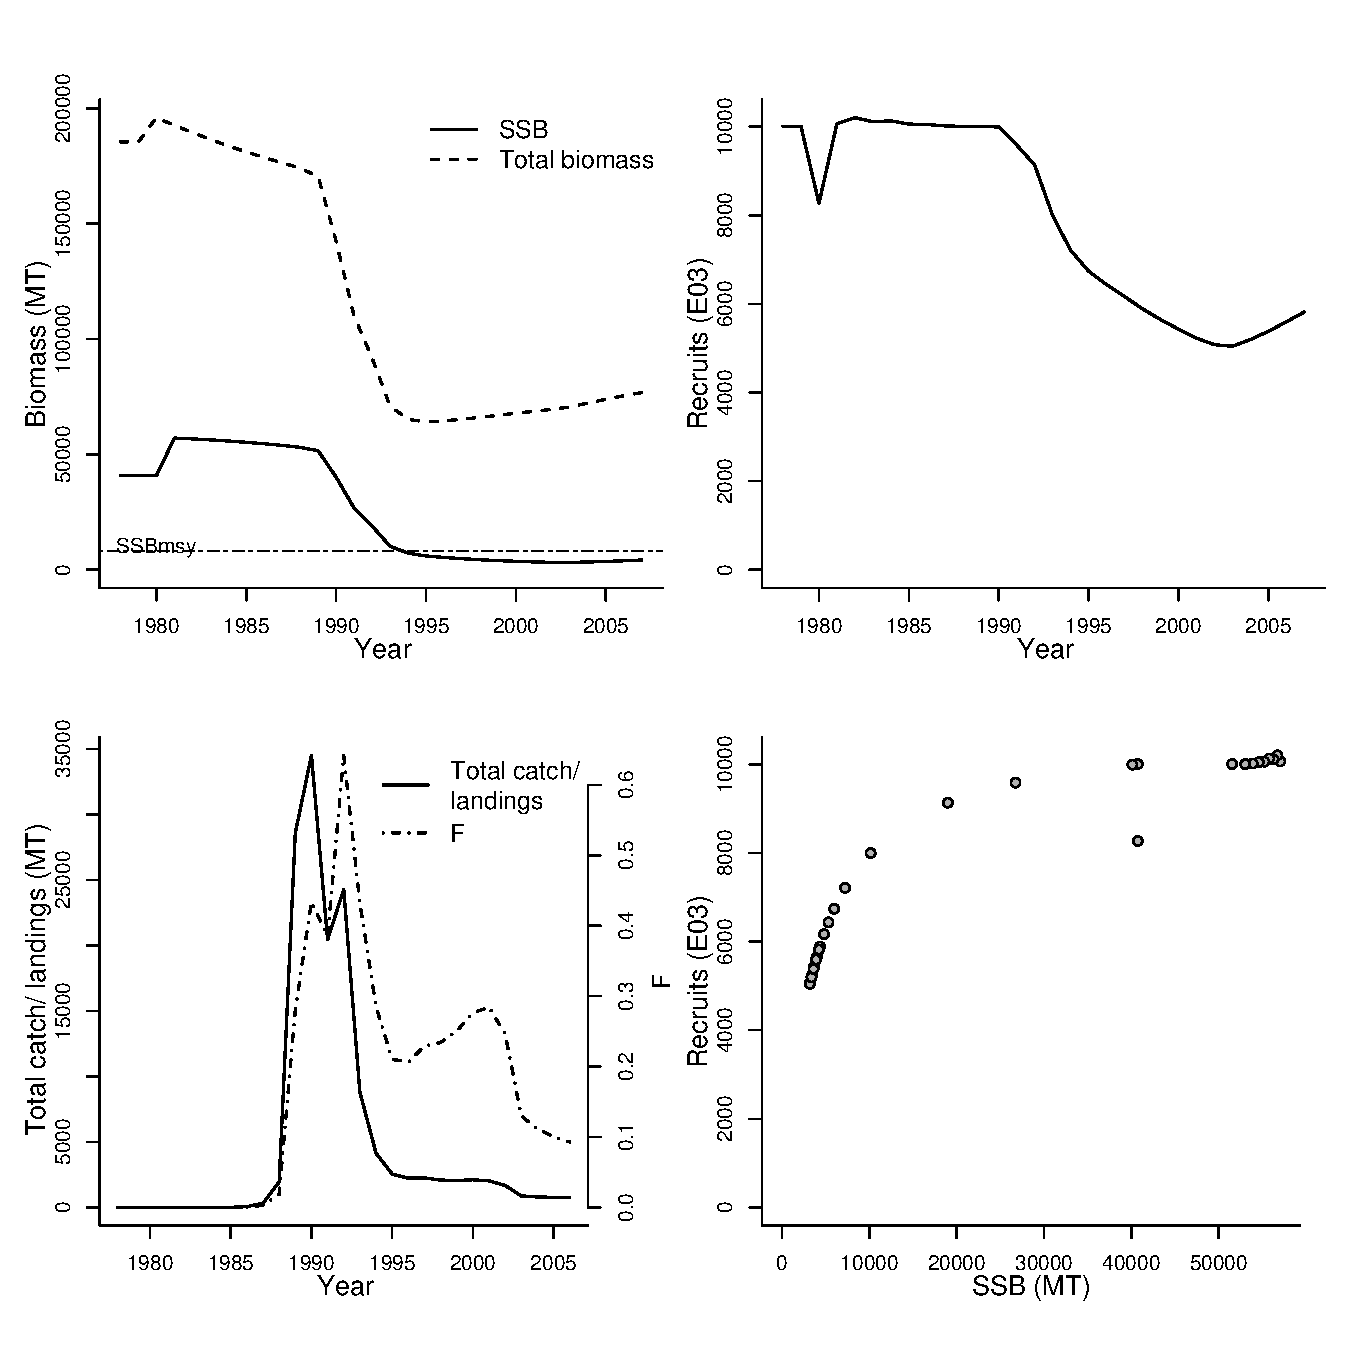
\includegraphics[scale=0.65]{../tex/figures/plot-CSIRO-OROUGHYSESSF-1978-2007-FULTON.pdf}
\end{center}

\newpage
\section{Clupeiformes}\index{Clupeiformes}

\subsection{Clupeidae}\index{Clupeidae}\index{Clupeiformes!Clupeidae}

\subsubsection{Clupea harengus - Herring}\index{Herring}\index{Clupea harengus}\index{Clupeidae!Clupea harengus}
ID: WGBFAS-HERRIsum-1983-2007-JENNINGS

Herring Iceland (Summer spawners) 

stock assessment conducted: VPA/ADPAT version 2.3.2 NOAA Fisheries 
\begin{center}
\vspace{-0.2cm}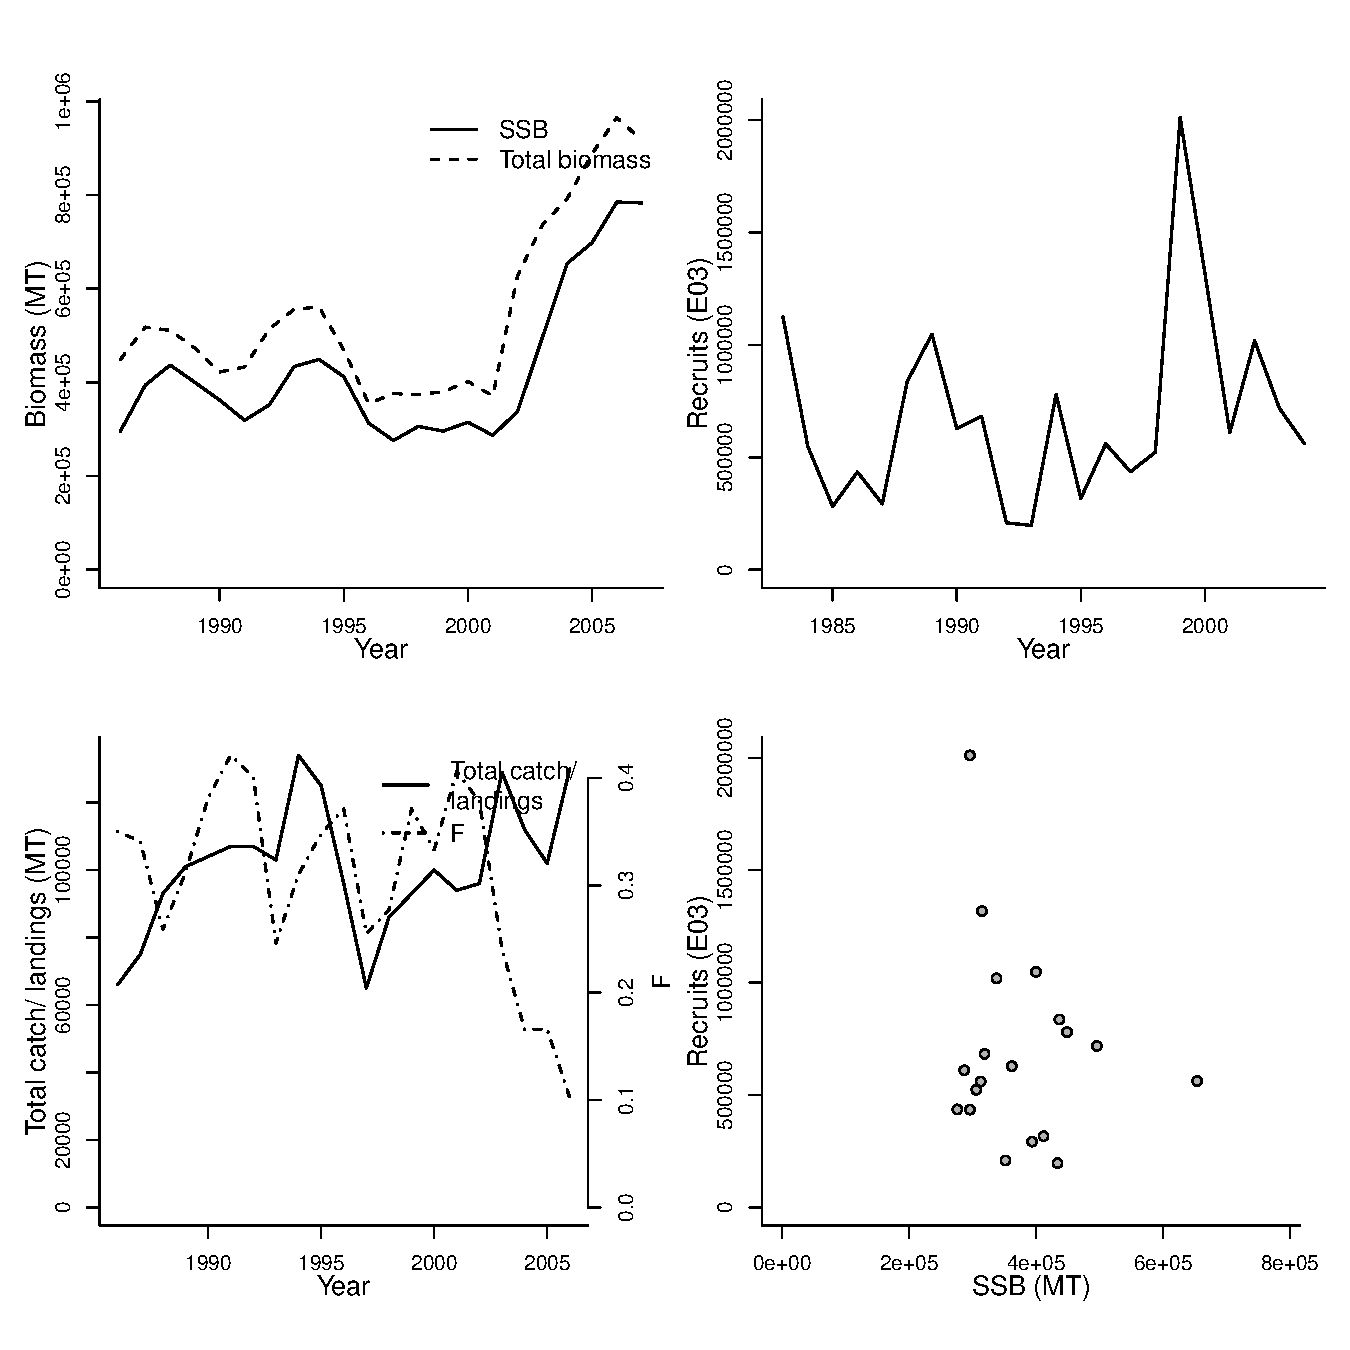
\includegraphics[scale=0.65]{../tex/figures/plot-WGBFAS-HERRIsum-1983-2007-JENNINGS.pdf}
\end{center}

\newpage
\subsubsection{Clupea harengus - Herring}\index{Herring}\index{Clupea harengus}\index{Clupeidae!Clupea harengus}
ID: WGBFAS-HERR2532-1973-2006-JENNINGS

Herring ICES 25-32 

stock assessment conducted: Extended Survivor Analysis 
\begin{center}
\vspace{-0.2cm}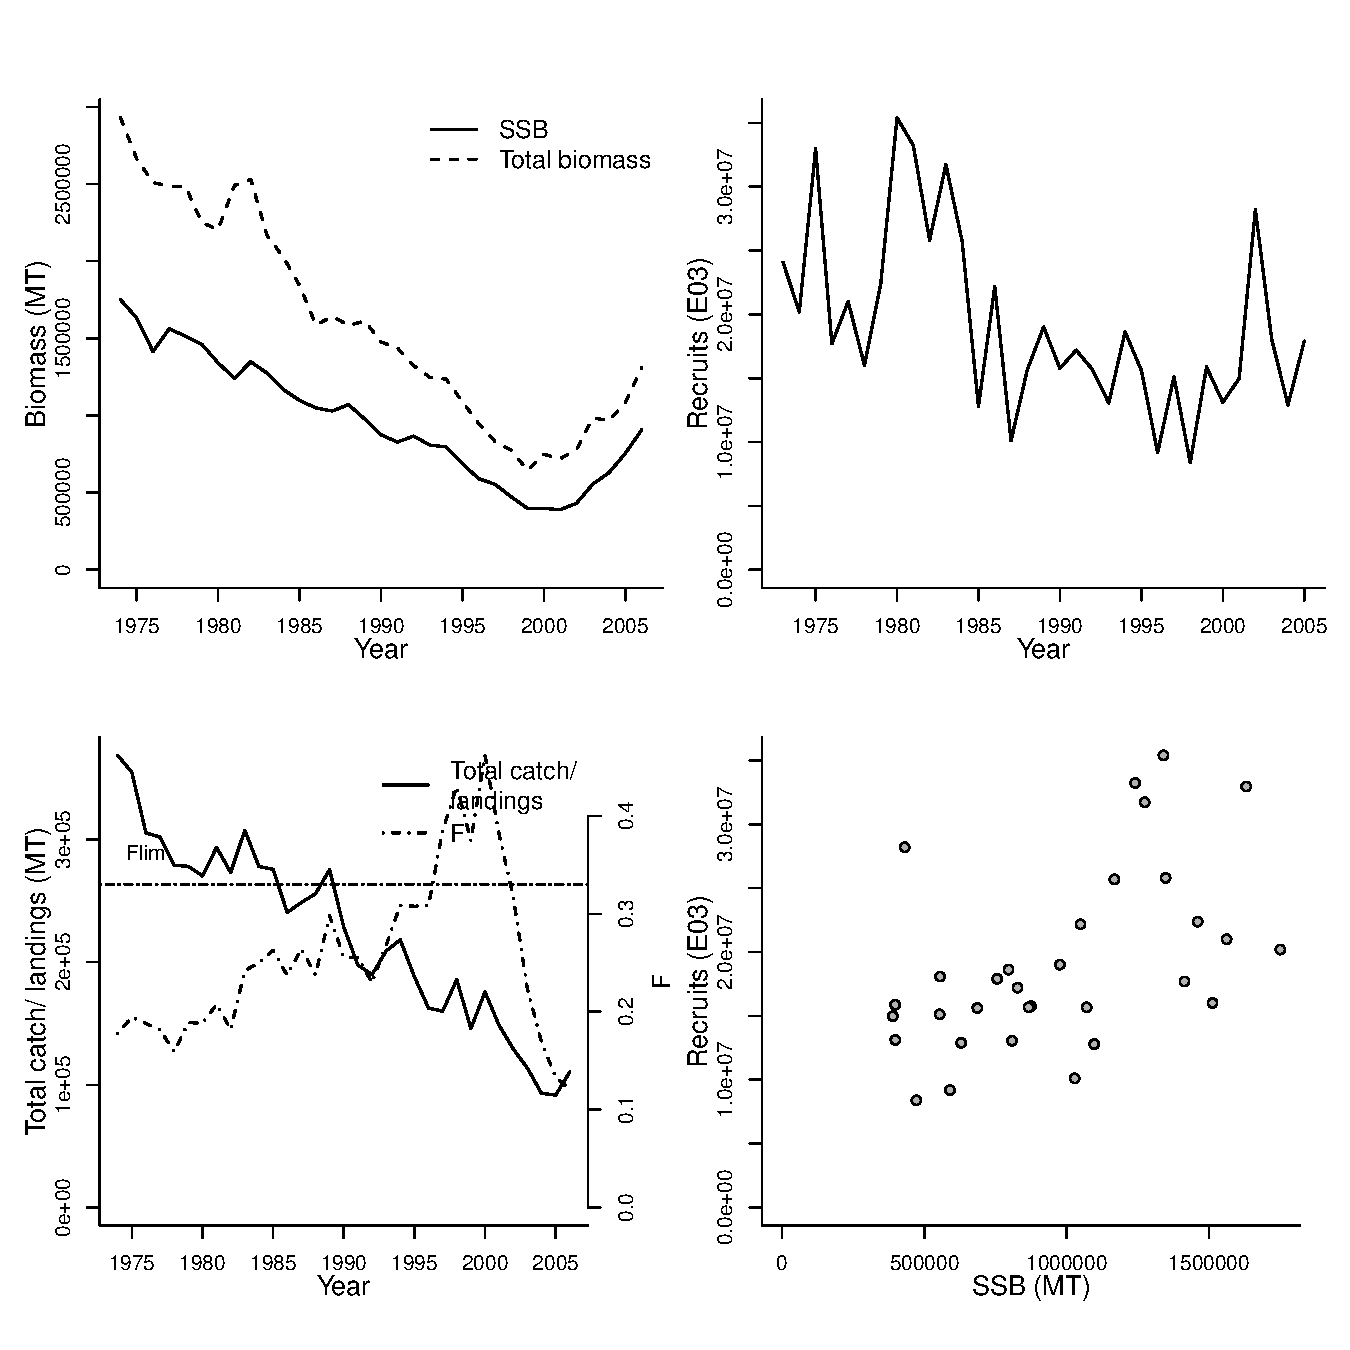
\includegraphics[scale=0.65]{../tex/figures/plot-WGBFAS-HERR2532-1973-2006-JENNINGS.pdf}
\end{center}

\newpage
\subsubsection{Clupea harengus - Herring}\index{Herring}\index{Clupea harengus}\index{Clupeidae!Clupea harengus}
ID: WGBFAS-HERRRIGA-1976-2007-JENNINGS

Herring ICES 28 

stock assessment conducted: Extended Survivor Analysis 
\begin{center}
\vspace{-0.2cm}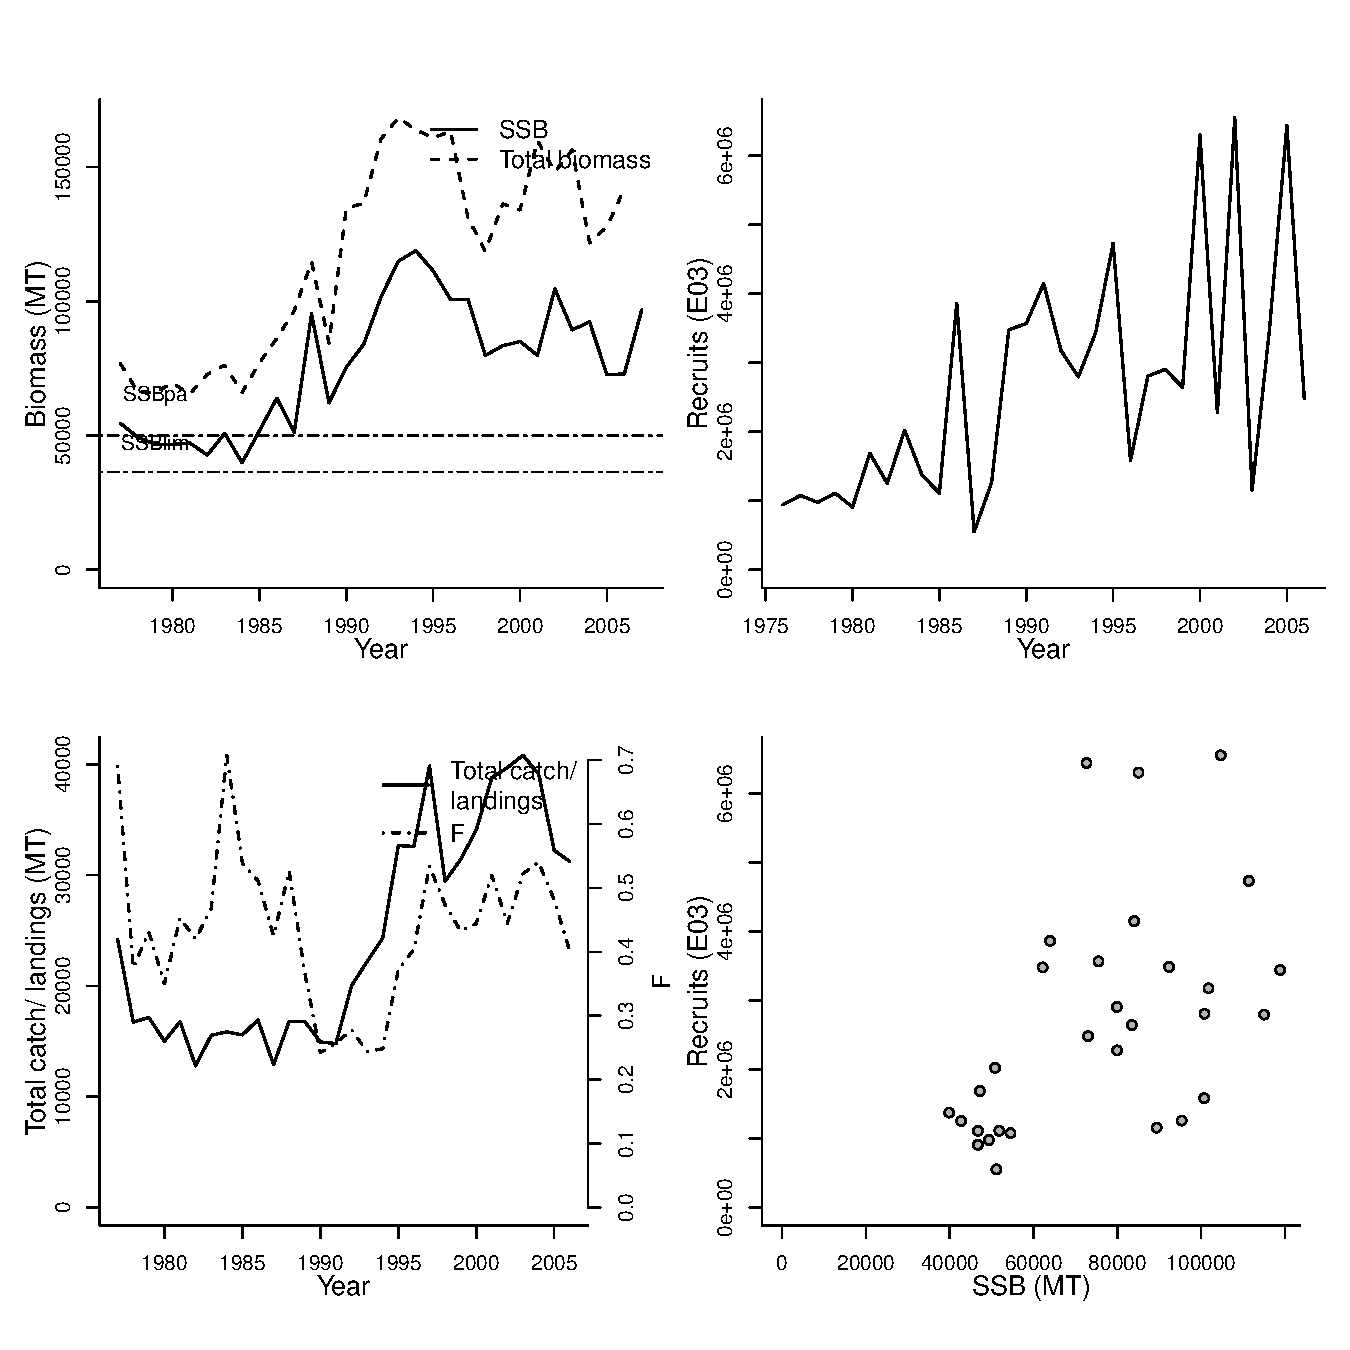
\includegraphics[scale=0.65]{../tex/figures/plot-WGBFAS-HERRRIGA-1976-2007-JENNINGS.pdf}
\end{center}

\newpage
\subsubsection{Clupea harengus - Herring}\index{Herring}\index{Clupea harengus}\index{Clupeidae!Clupea harengus}
ID: WGBFAS-HERR30-1972-2007-JENNINGS

Herring ICES 30 

stock assessment conducted: Extended Survivor Analysis 
\begin{center}
\vspace{-0.2cm}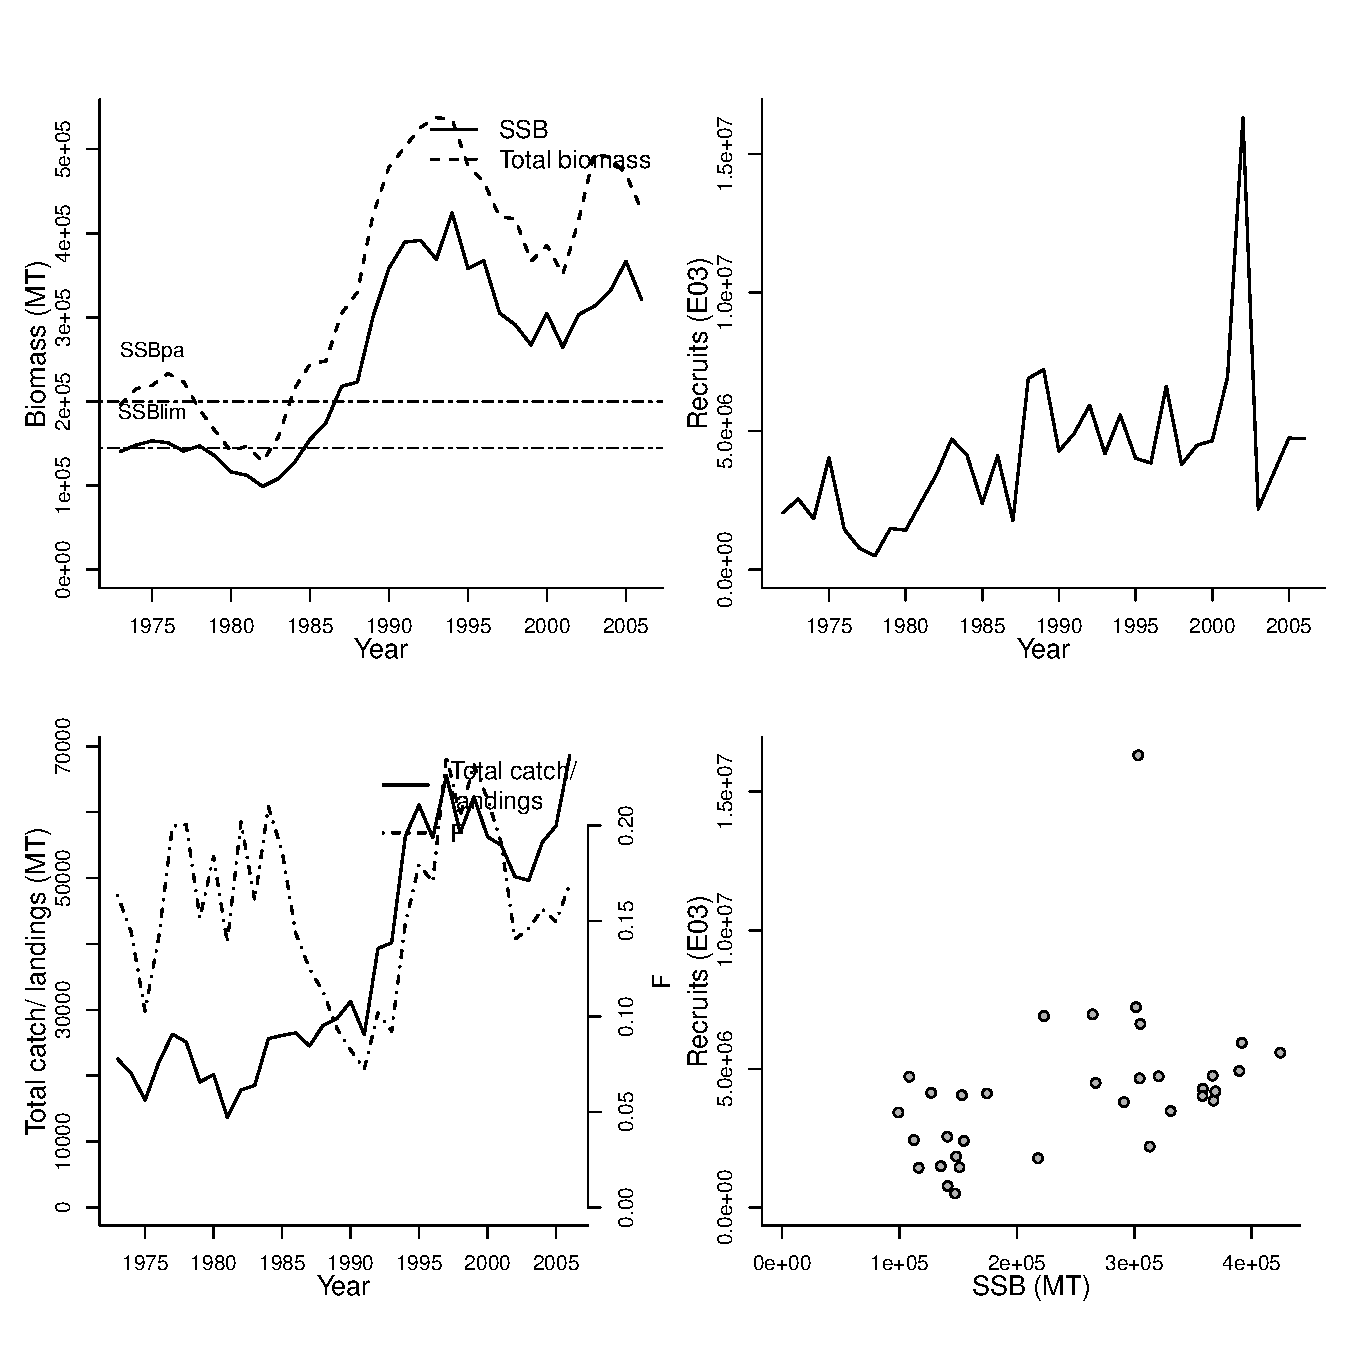
\includegraphics[scale=0.65]{../tex/figures/plot-WGBFAS-HERR30-1972-2007-JENNINGS.pdf}
\end{center}

\newpage
\subsubsection{Clupea harengus - Herring}\index{Herring}\index{Clupea harengus}\index{Clupeidae!Clupea harengus}
ID: WGBFAS-HERR31-1979-2006-JENNINGS

Herring ICES 31 

stock assessment conducted: Extended Survivor Analysis 
\begin{center}
\vspace{-0.2cm}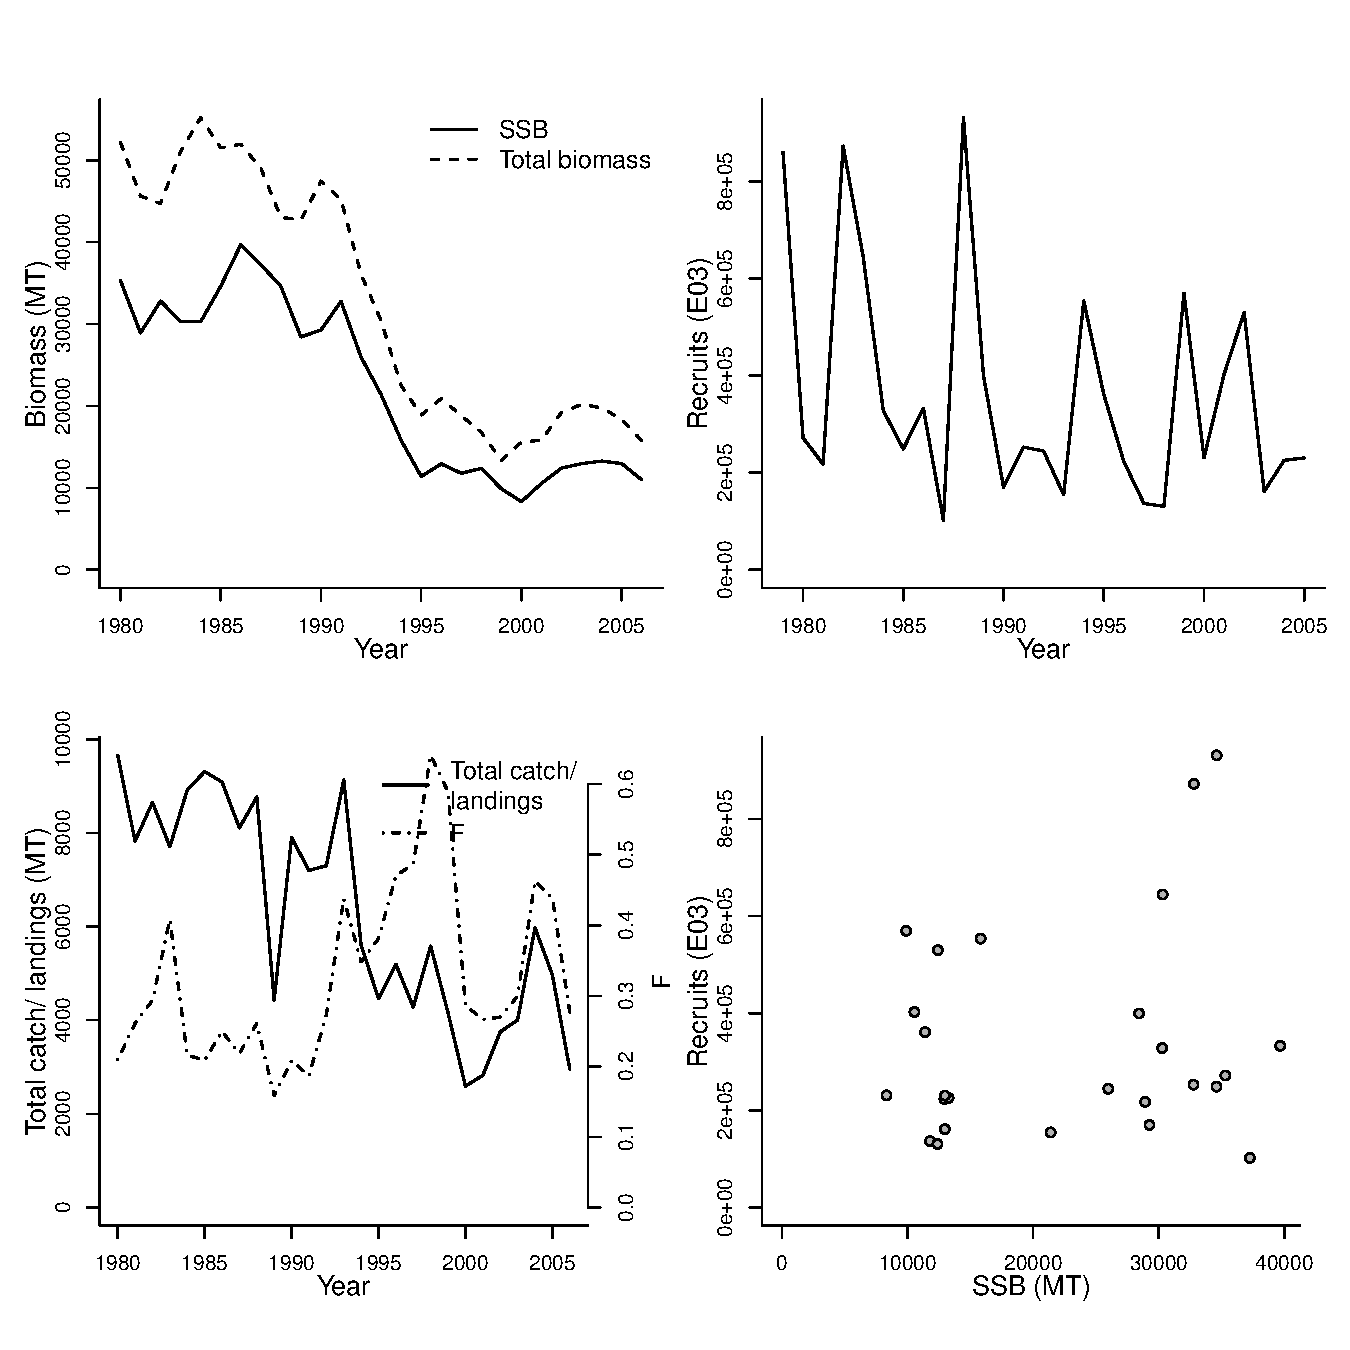
\includegraphics[scale=0.65]{../tex/figures/plot-WGBFAS-HERR31-1979-2006-JENNINGS.pdf}
\end{center}

\newpage
\subsubsection{Clupea harengus - Herring}\index{Herring}\index{Clupea harengus}\index{Clupeidae!Clupea harengus}
ID: HAWG-HERRNIRS-1960-2006-JENNINGS

Herring Northern Irish Sea 

stock assessment conducted: Integrated Catch-at-age Analysis 
\begin{center}
\vspace{-0.2cm}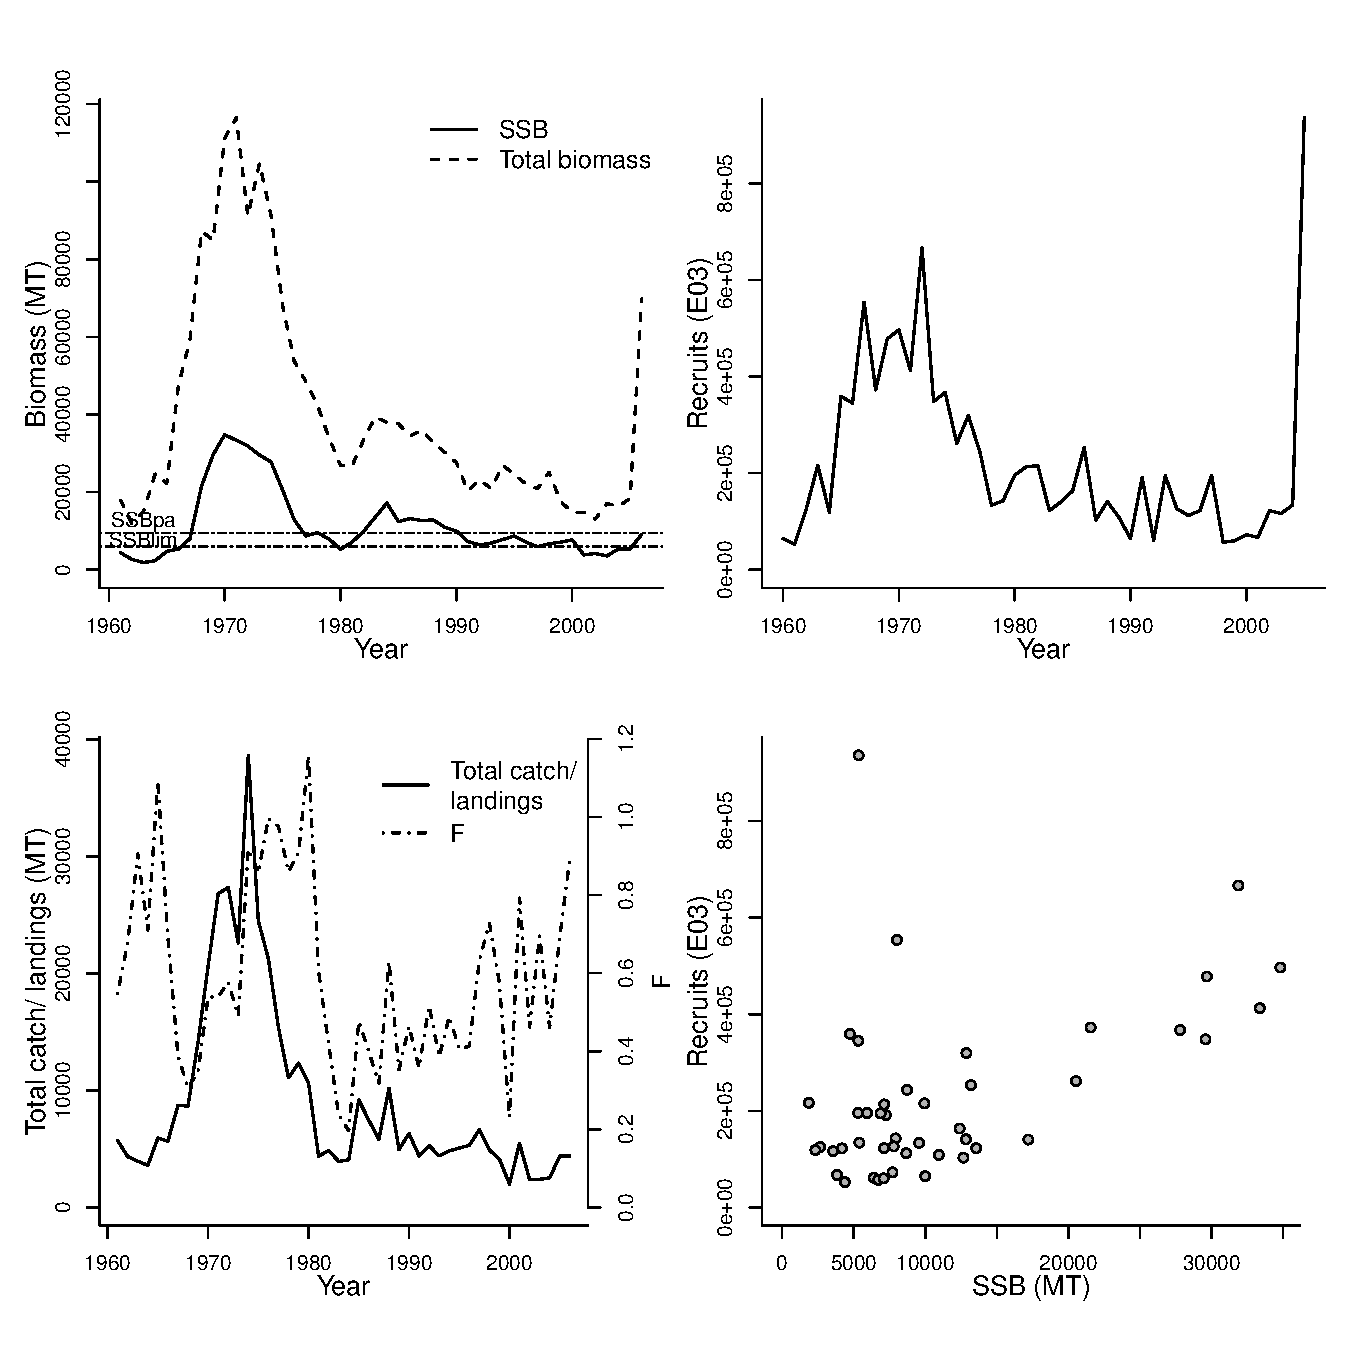
\includegraphics[scale=0.65]{../tex/figures/plot-HAWG-HERRNIRS-1960-2006-JENNINGS.pdf}
\end{center}

\newpage
\subsubsection{Clupea pallasii - Pacific herring}\index{Pacific herring}\index{Clupea pallasii}\index{Clupeidae!Clupea pallasii}
ID: DFO-PAC-HERRCC-1951-2007-COLLIE

Pacific herring Central Coast 

stock assessment conducted: an AD-Model builder statistical Catch at Age Model 
\begin{center}
\vspace{-0.2cm}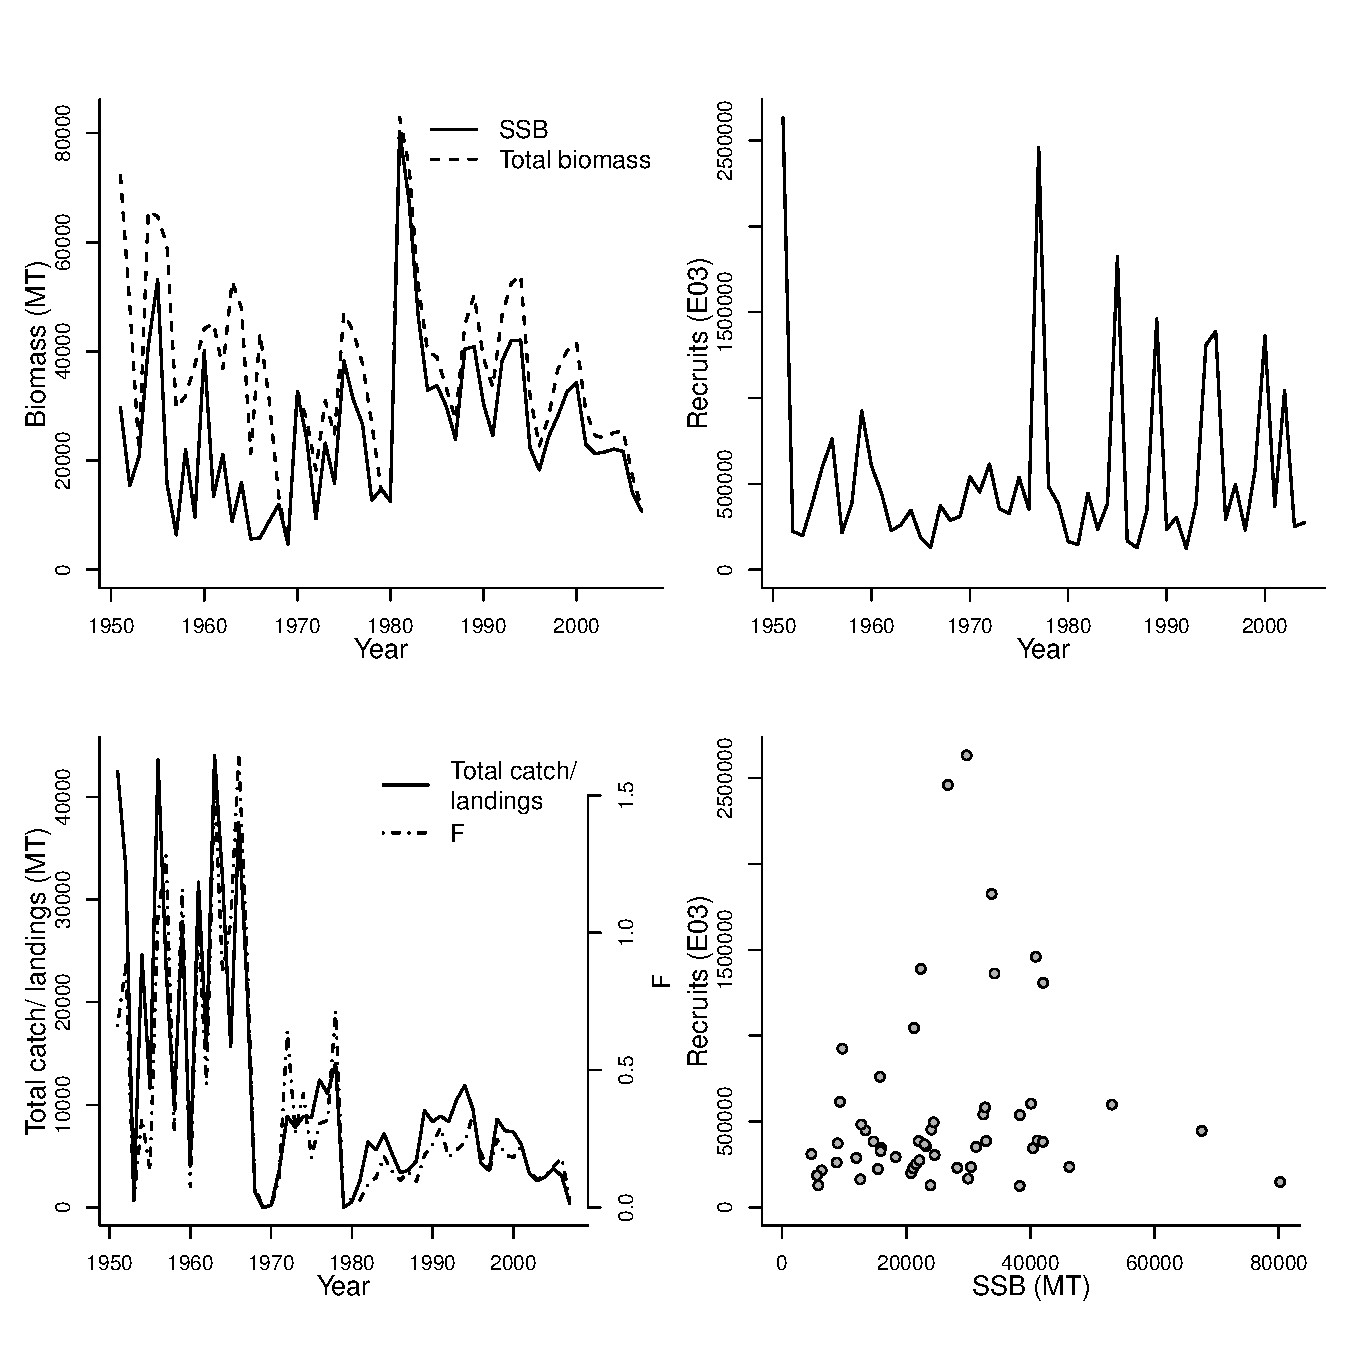
\includegraphics[scale=0.65]{../tex/figures/plot-DFO-PAC-HERRCC-1951-2007-COLLIE.pdf}
\end{center}

\newpage
\subsubsection{Clupea pallasii - Pacific herring}\index{Pacific herring}\index{Clupea pallasii}\index{Clupeidae!Clupea pallasii}
ID: DFO-PAC-HERRPRD-1951-2007-COLLIE

Pacific herring Prince Rupert District 

stock assessment conducted: an AD-Model builder statistical Catch at Age Model 
\begin{center}
\vspace{-0.2cm}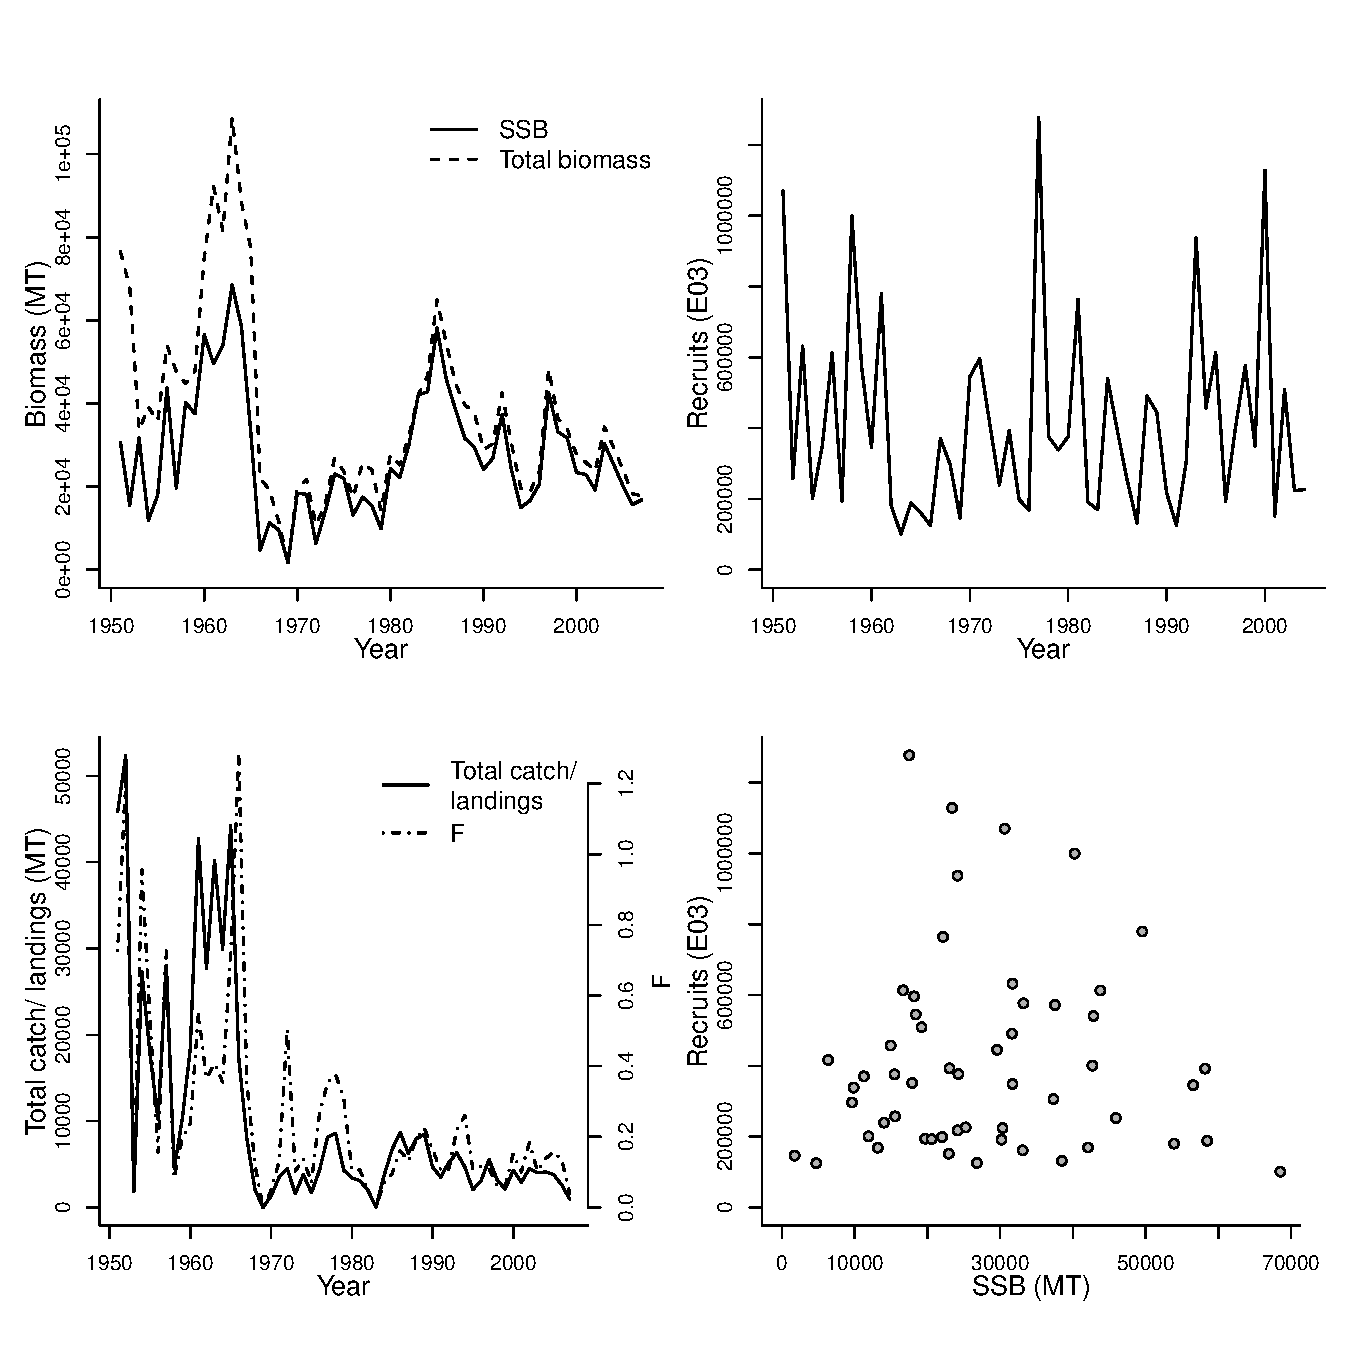
\includegraphics[scale=0.65]{../tex/figures/plot-DFO-PAC-HERRPRD-1951-2007-COLLIE.pdf}
\end{center}

\newpage
\subsubsection{Clupea pallasii - Pacific herring}\index{Pacific herring}\index{Clupea pallasii}\index{Clupeidae!Clupea pallasii}
ID: DFO-PAC-HERRQCI-1951-2007-COLLIE

Pacific herring Queen Charlotte Islands 

stock assessment conducted: an AD-Model builder statistical Catch at Age Model 
\begin{center}
\vspace{-0.2cm}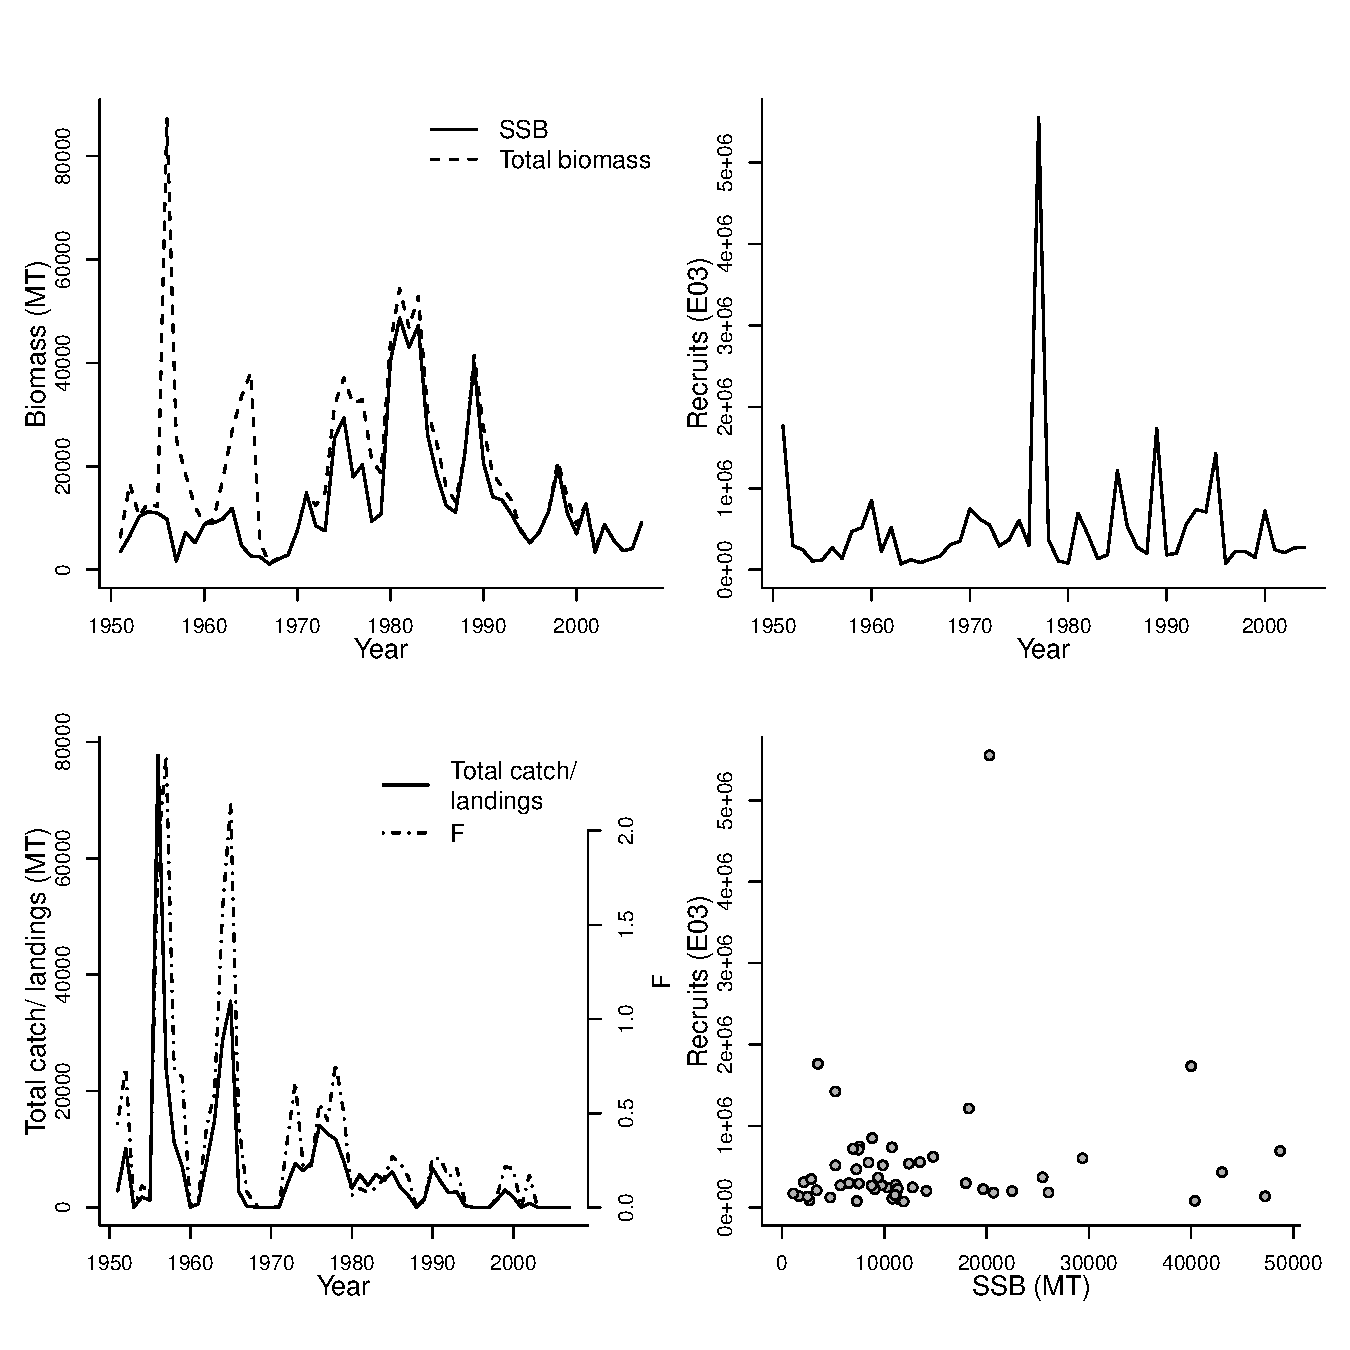
\includegraphics[scale=0.65]{../tex/figures/plot-DFO-PAC-HERRQCI-1951-2007-COLLIE.pdf}
\end{center}

\newpage
\subsubsection{Clupea pallasii - Pacific herring}\index{Pacific herring}\index{Clupea pallasii}\index{Clupeidae!Clupea pallasii}
ID: DFO-PAC-HERRSOG-1951-2007-COLLIE

Pacific herring Straight of Georgia 

stock assessment conducted: an AD-Model builder statistical Catch at Age Model 
\begin{center}
\vspace{-0.2cm}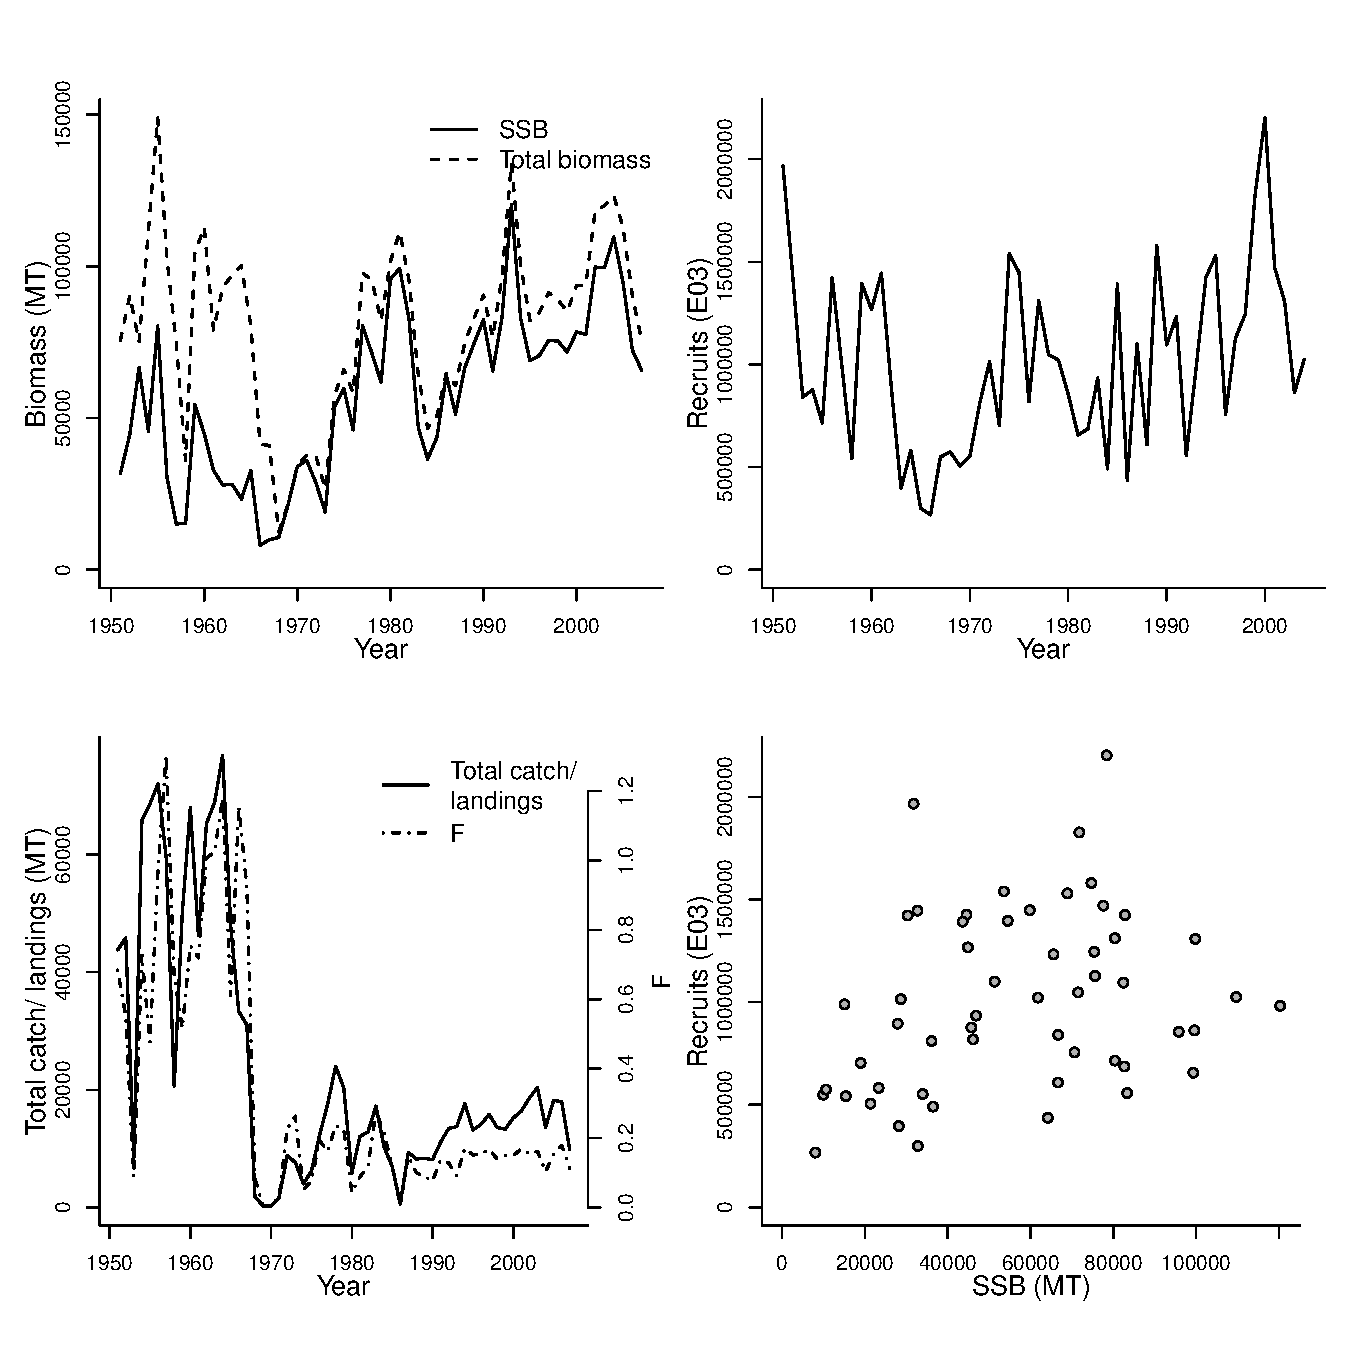
\includegraphics[scale=0.65]{../tex/figures/plot-DFO-PAC-HERRSOG-1951-2007-COLLIE.pdf}
\end{center}

\newpage
\subsubsection{Clupea pallasii - Pacific herring}\index{Pacific herring}\index{Clupea pallasii}\index{Clupeidae!Clupea pallasii}
ID: DFO-PAC-HERRWCVANI-1951-2007-COLLIE

Pacific herring West Coast of Vancouver Island 

stock assessment conducted: an AD-Model builder statistical Catch at Age Model 
\begin{center}
\vspace{-0.2cm}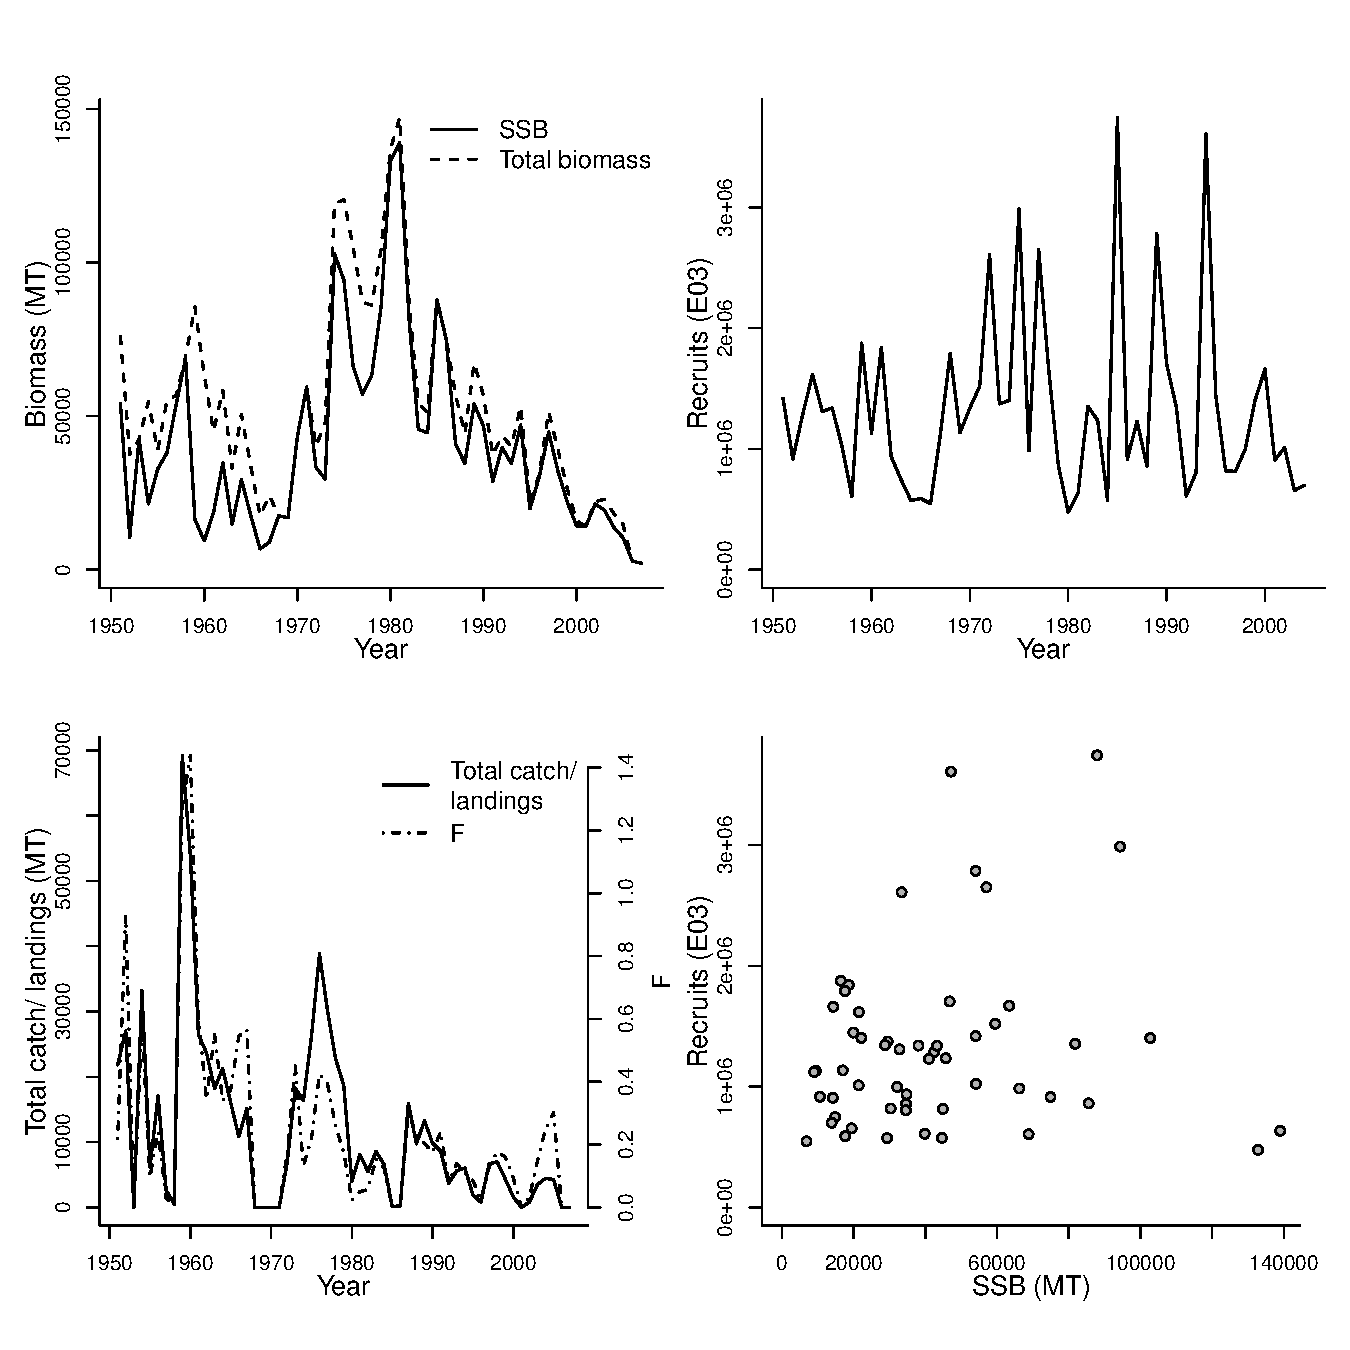
\includegraphics[scale=0.65]{../tex/figures/plot-DFO-PAC-HERRWCVANI-1951-2007-COLLIE.pdf}
\end{center}

\newpage
\subsubsection{Sardina pilchardus - European pilchard}\index{European pilchard}\index{Sardina pilchardus}\index{Clupeidae!Sardina pilchardus}
ID: WGMHSA-SARDPVIIIc-IXa-1978-2007-JENNINGS

European pilchard ICES VIIIc-IXa 

stock assessment conducted: a flexible age structured model 
\begin{center}
\vspace{-0.2cm}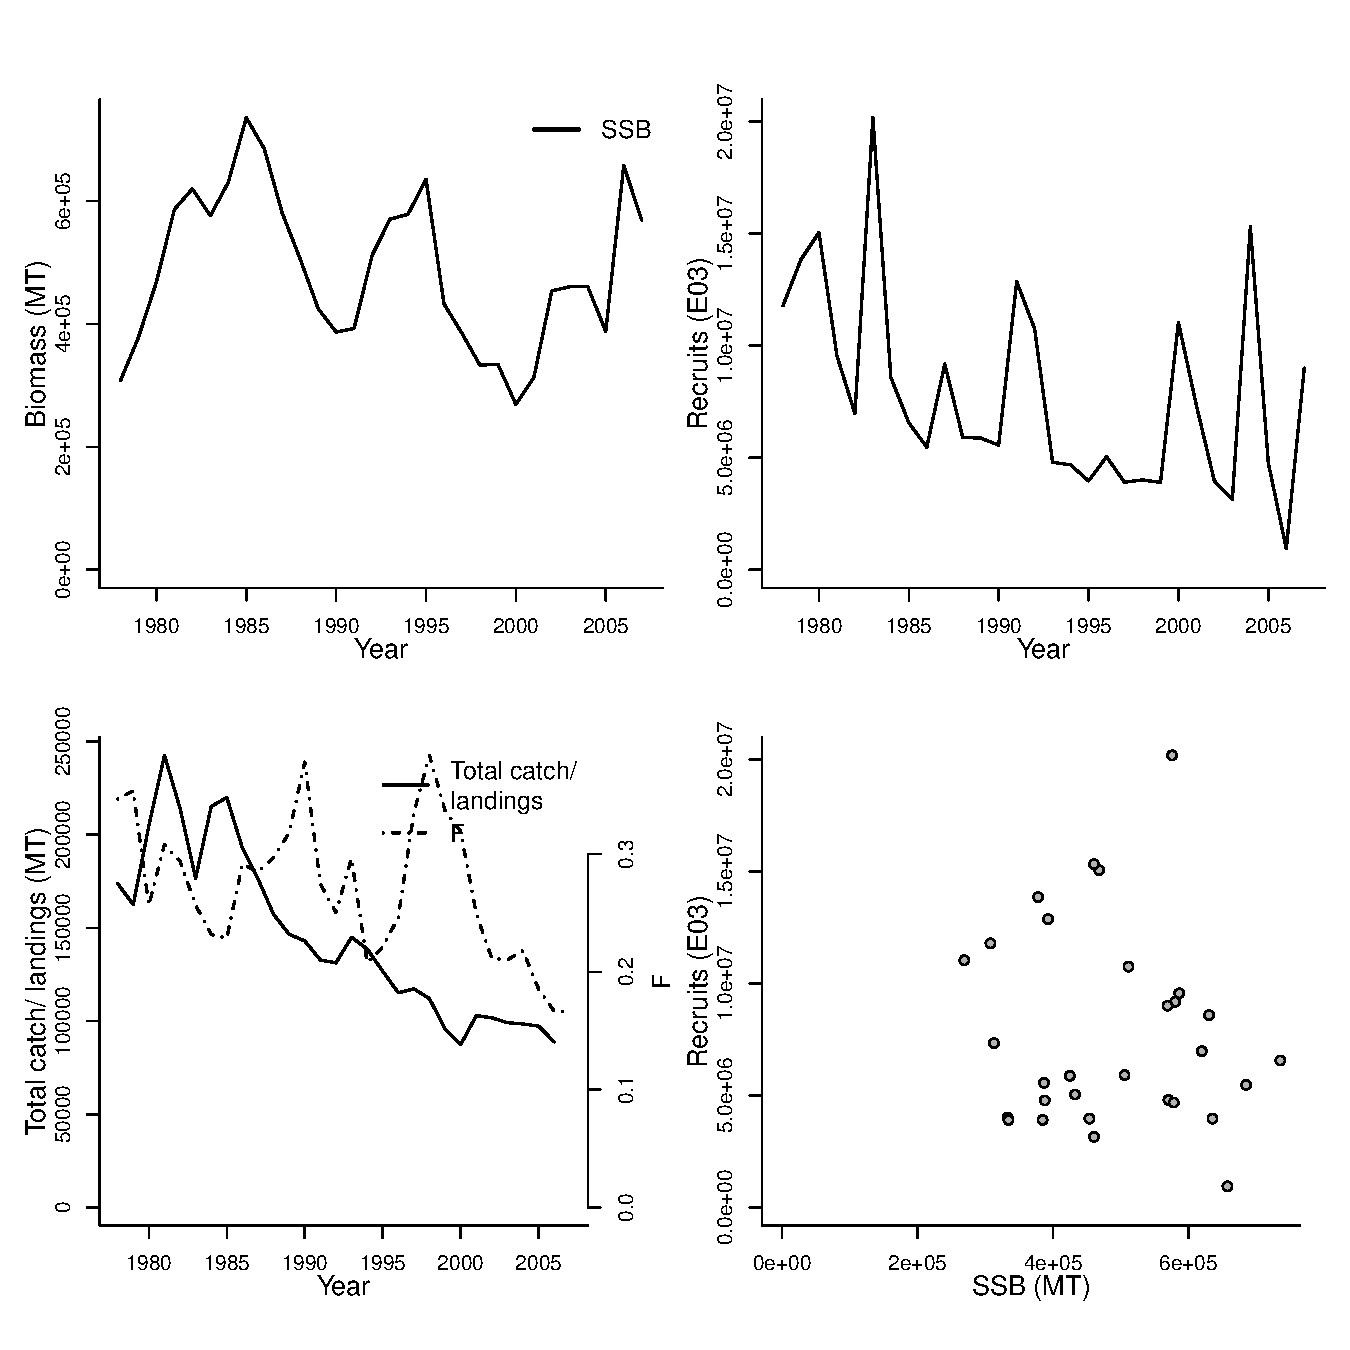
\includegraphics[scale=0.65]{../tex/figures/plot-WGMHSA-SARDPVIIIc-IXa-1978-2007-JENNINGS.pdf}
\end{center}

\newpage
\subsubsection{Sprattus sprattus - Sprat}\index{Sprat}\index{Sprattus sprattus}\index{Clupeidae!Sprattus sprattus}
ID: WGBFAS-SPRAT22-32-1973-2007-JENNINGS

Sprat ICES Baltic Areas 22-32 

stock assessment conducted: Extended Survivor Analysis 
\begin{center}
\vspace{-0.2cm}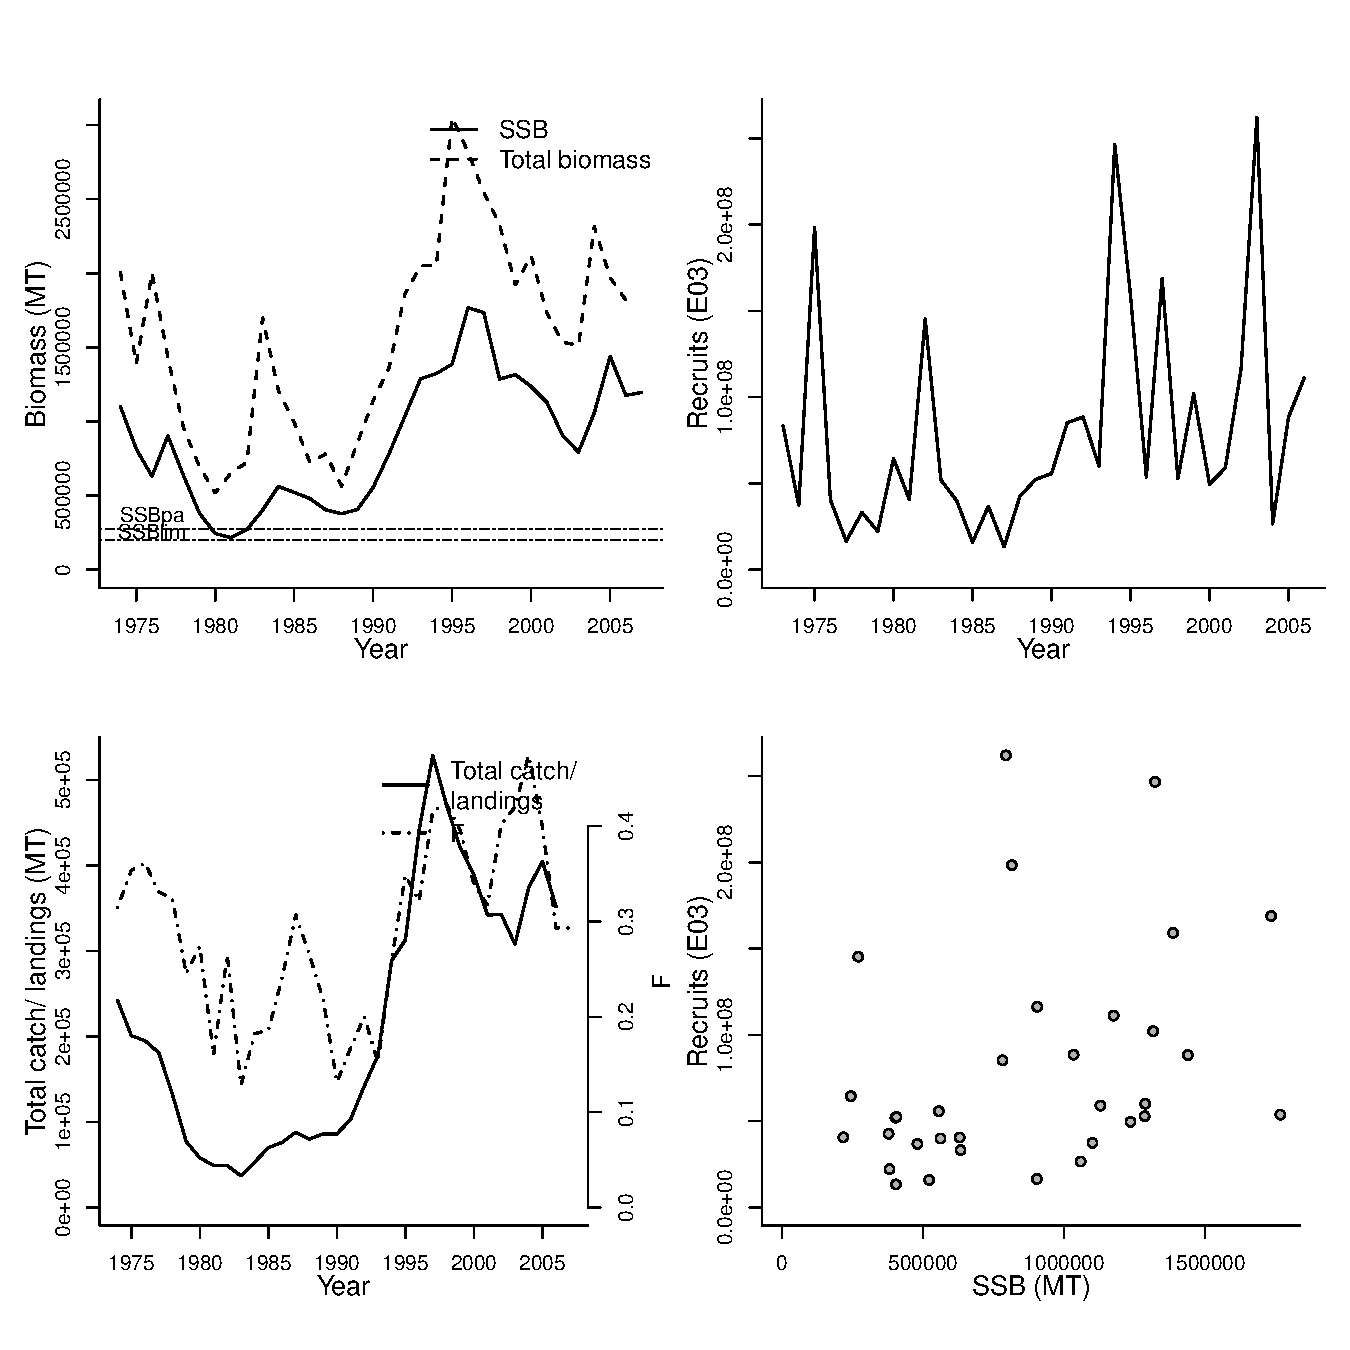
\includegraphics[scale=0.65]{../tex/figures/plot-WGBFAS-SPRAT22-32-1973-2007-JENNINGS.pdf}
\end{center}

\newpage
\subsection{Engraulidae}\index{Engraulidae}\index{Clupeiformes!Engraulidae}

\subsubsection{Engraulis anchoita - Argentine anchoita}\index{Argentine anchoita}\index{Engraulis anchoita}\index{Engraulidae!Engraulis anchoita}
ID: INIDEP-ARGANCHONARG-1989-2007-Parma

Argentine anchoita Northern Argentina 

stock assessment conducted: A general approach to fitting VPA models. ADAPT is based on minimising the sum-of-squares over any number of indices of abundance to find best-fit parameters. 
\begin{center}
\vspace{-0.2cm}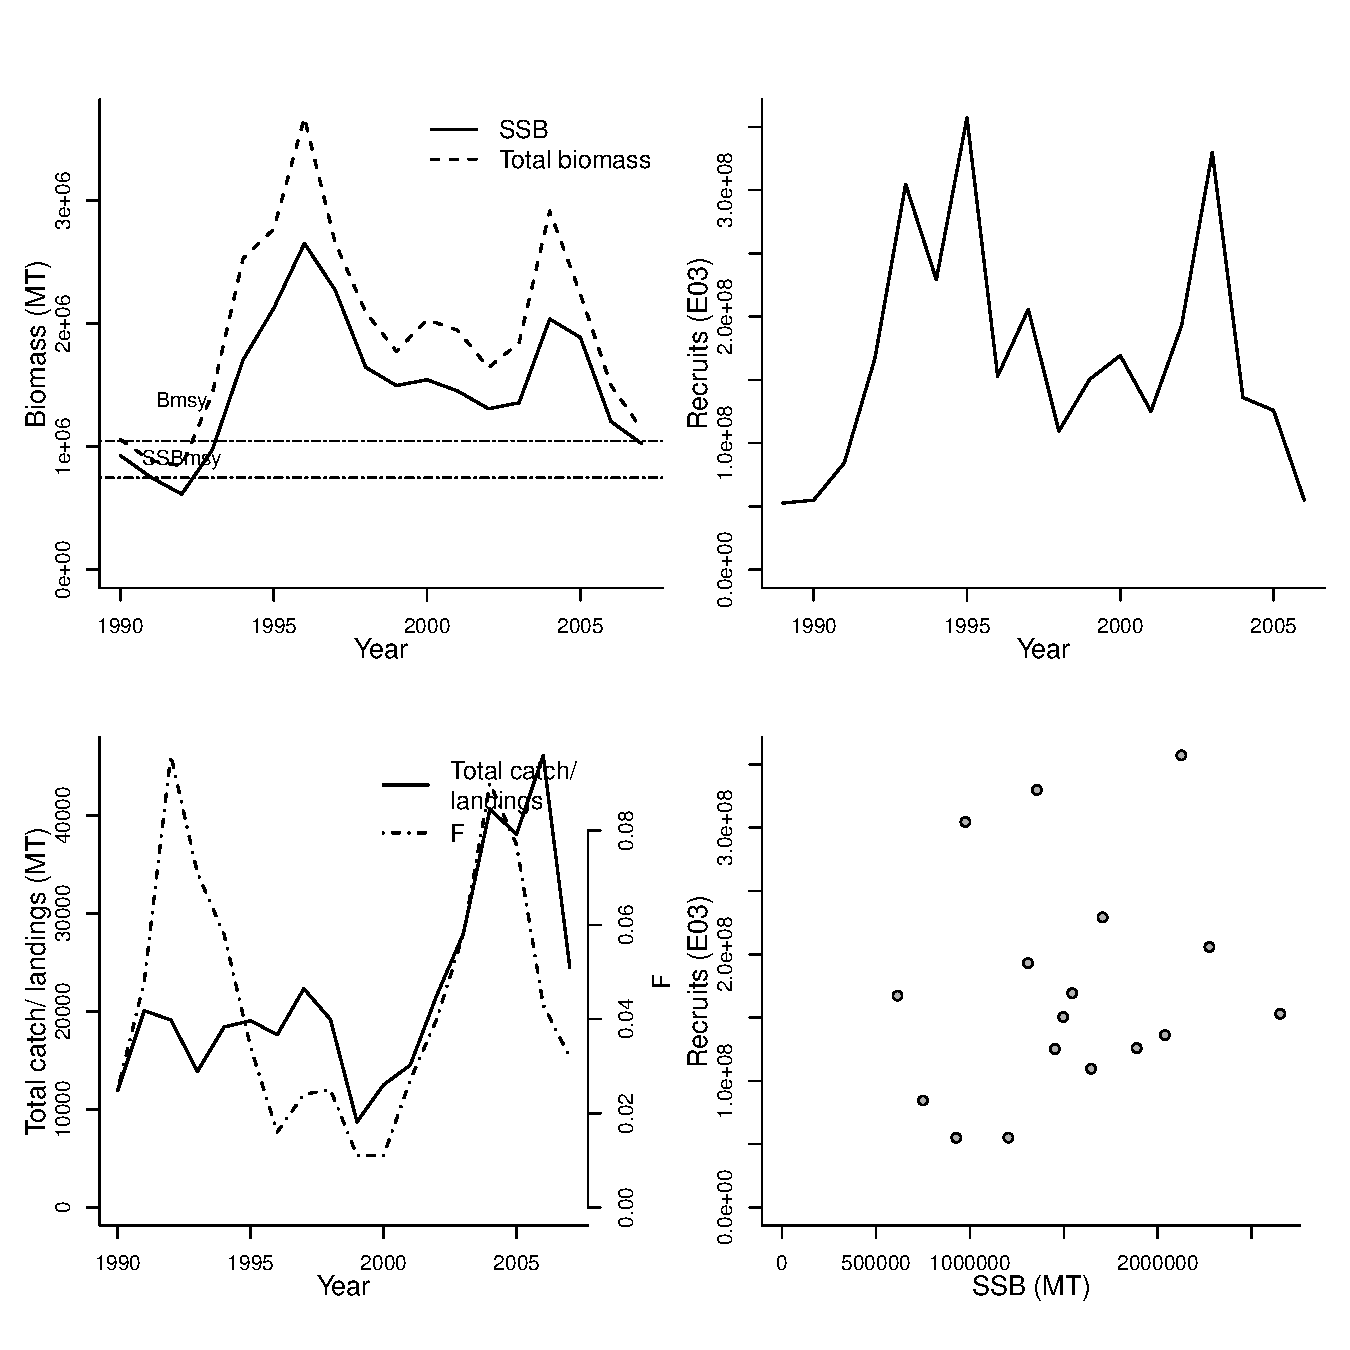
\includegraphics[scale=0.65]{../tex/figures/plot-INIDEP-ARGANCHONARG-1989-2007-Parma.pdf}
\end{center}

\newpage
\subsubsection{Engraulis anchoita - Argentine anchoita}\index{Argentine anchoita}\index{Engraulis anchoita}\index{Engraulidae!Engraulis anchoita}
ID: INIDEP-ARGANCHOSARG-1992-2007-Parma

Argentine anchoita Southern Argentina 

stock assessment conducted: Age-structured surplus production model 
\begin{center}
\vspace{-0.2cm}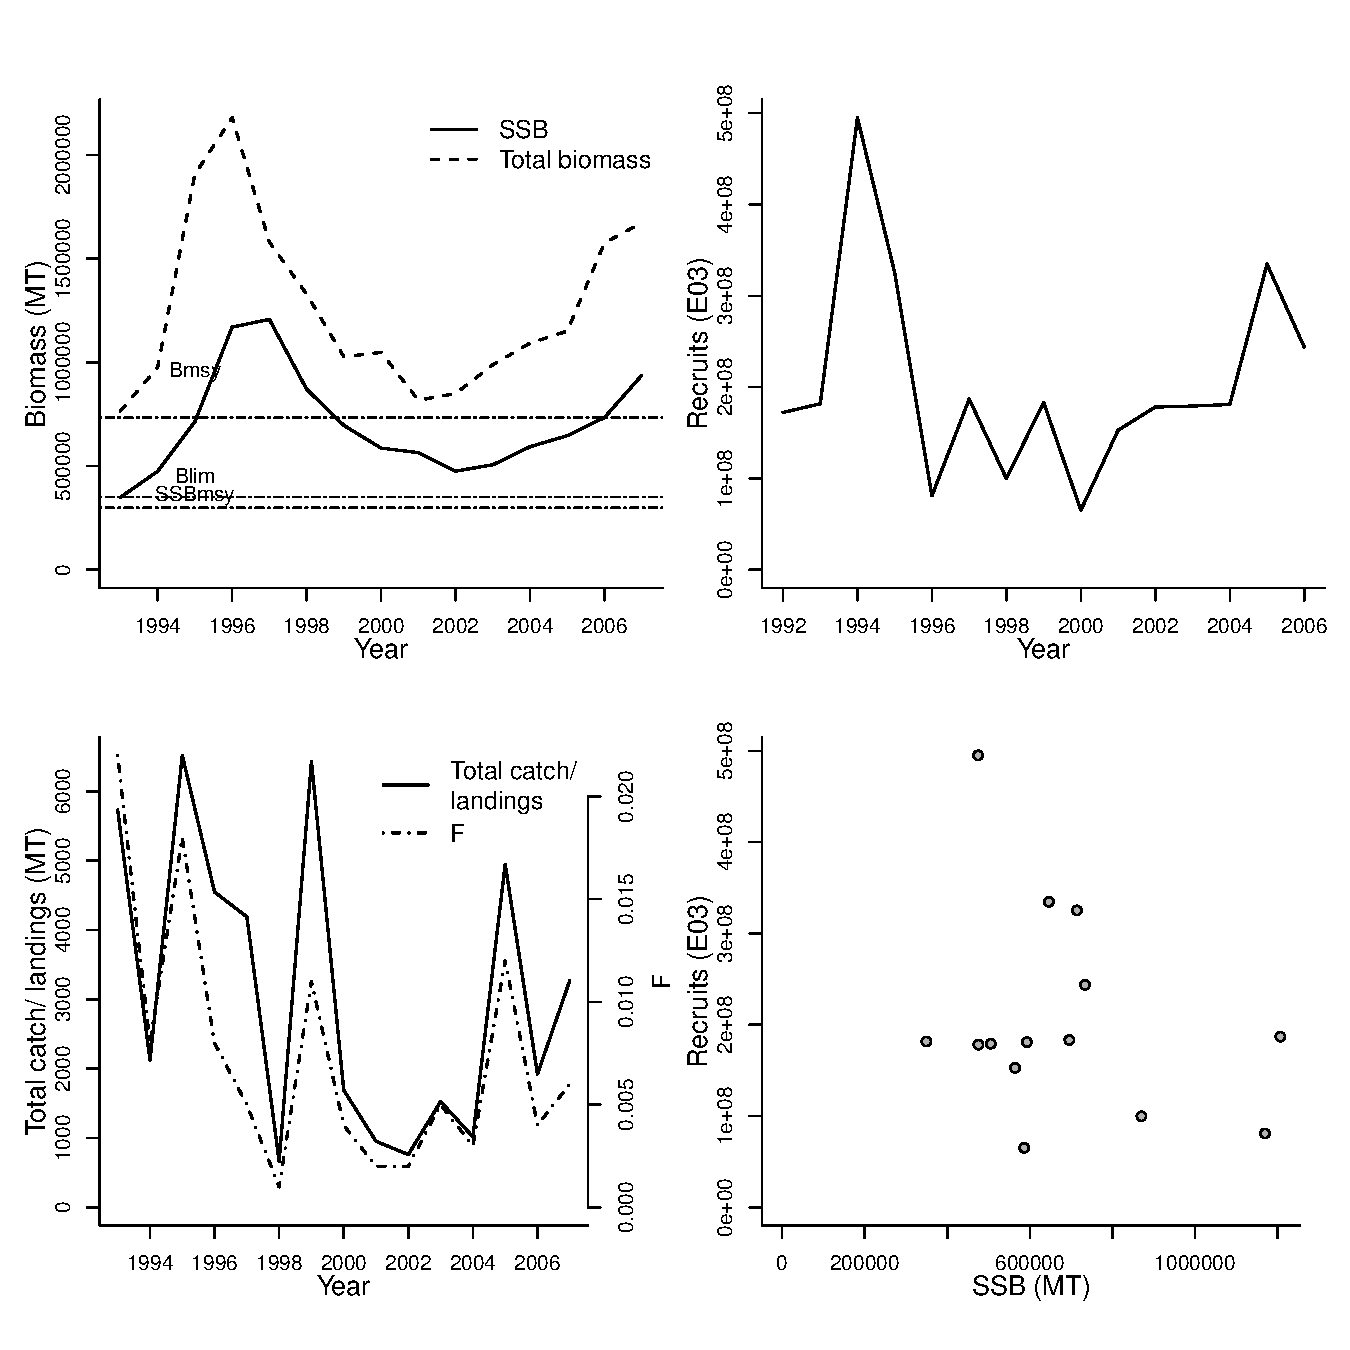
\includegraphics[scale=0.65]{../tex/figures/plot-INIDEP-ARGANCHOSARG-1992-2007-Parma.pdf}
\end{center}

\newpage
\subsubsection{Engraulis encrasicolus - Anchovy}\index{Anchovy}\index{Engraulis encrasicolus}\index{Engraulidae!Engraulis encrasicolus}
ID: WGMHSA-ANCHOBAYB-1986-2007-JENNINGS

Anchovy ICES VIII 

stock assessment conducted: Bayesian Biomass Model 
\begin{center}
\vspace{-0.2cm}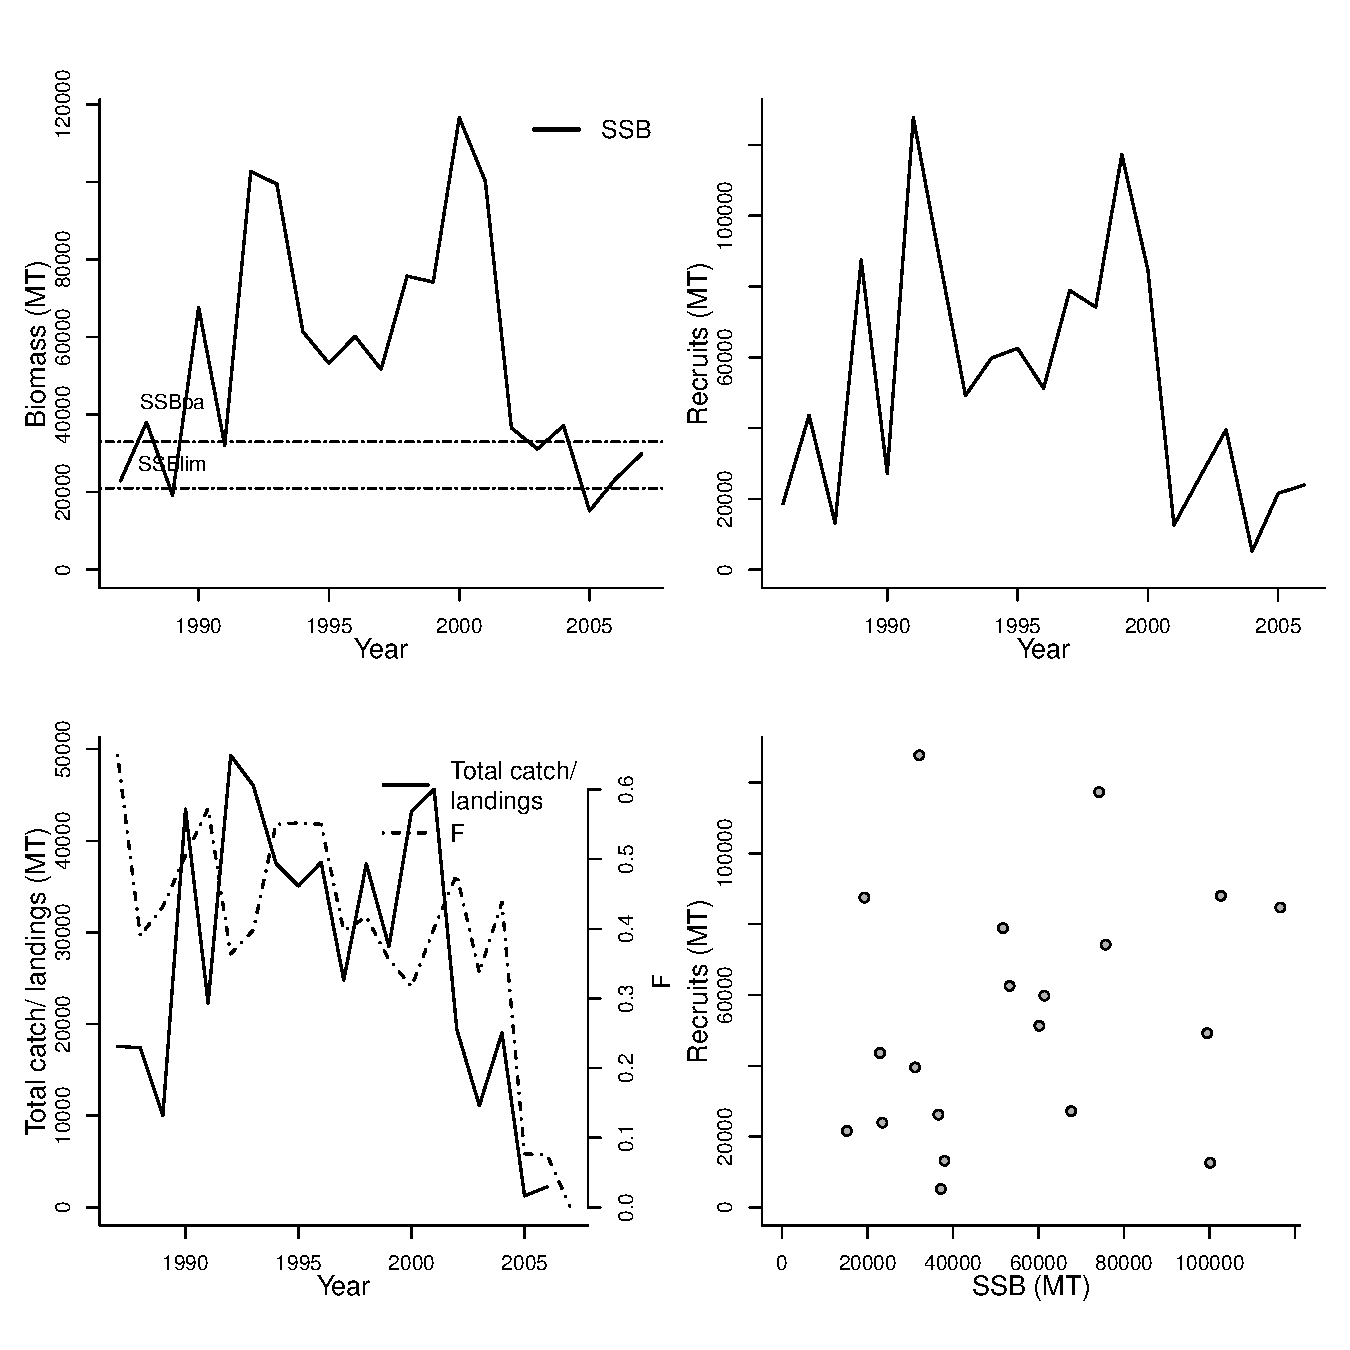
\includegraphics[scale=0.65]{../tex/figures/plot-WGMHSA-ANCHOBAYB-1986-2007-JENNINGS.pdf}
\end{center}

\newpage
\section{Decapoda}\index{Decapoda}

\subsection{Nephropidae}\index{Nephropidae}\index{Decapoda!Nephropidae}

\subsubsection{Homarus americanus - American lobster}\index{American lobster}\index{Homarus americanus}\index{Nephropidae!Homarus americanus}
ID: RIDEM-LOBSTERRI-1959-2007-COLLIE

American lobster Rhode Island 

stock assessment conducted: Age-aggregated surplus production model 
\begin{center}
\vspace{-0.2cm}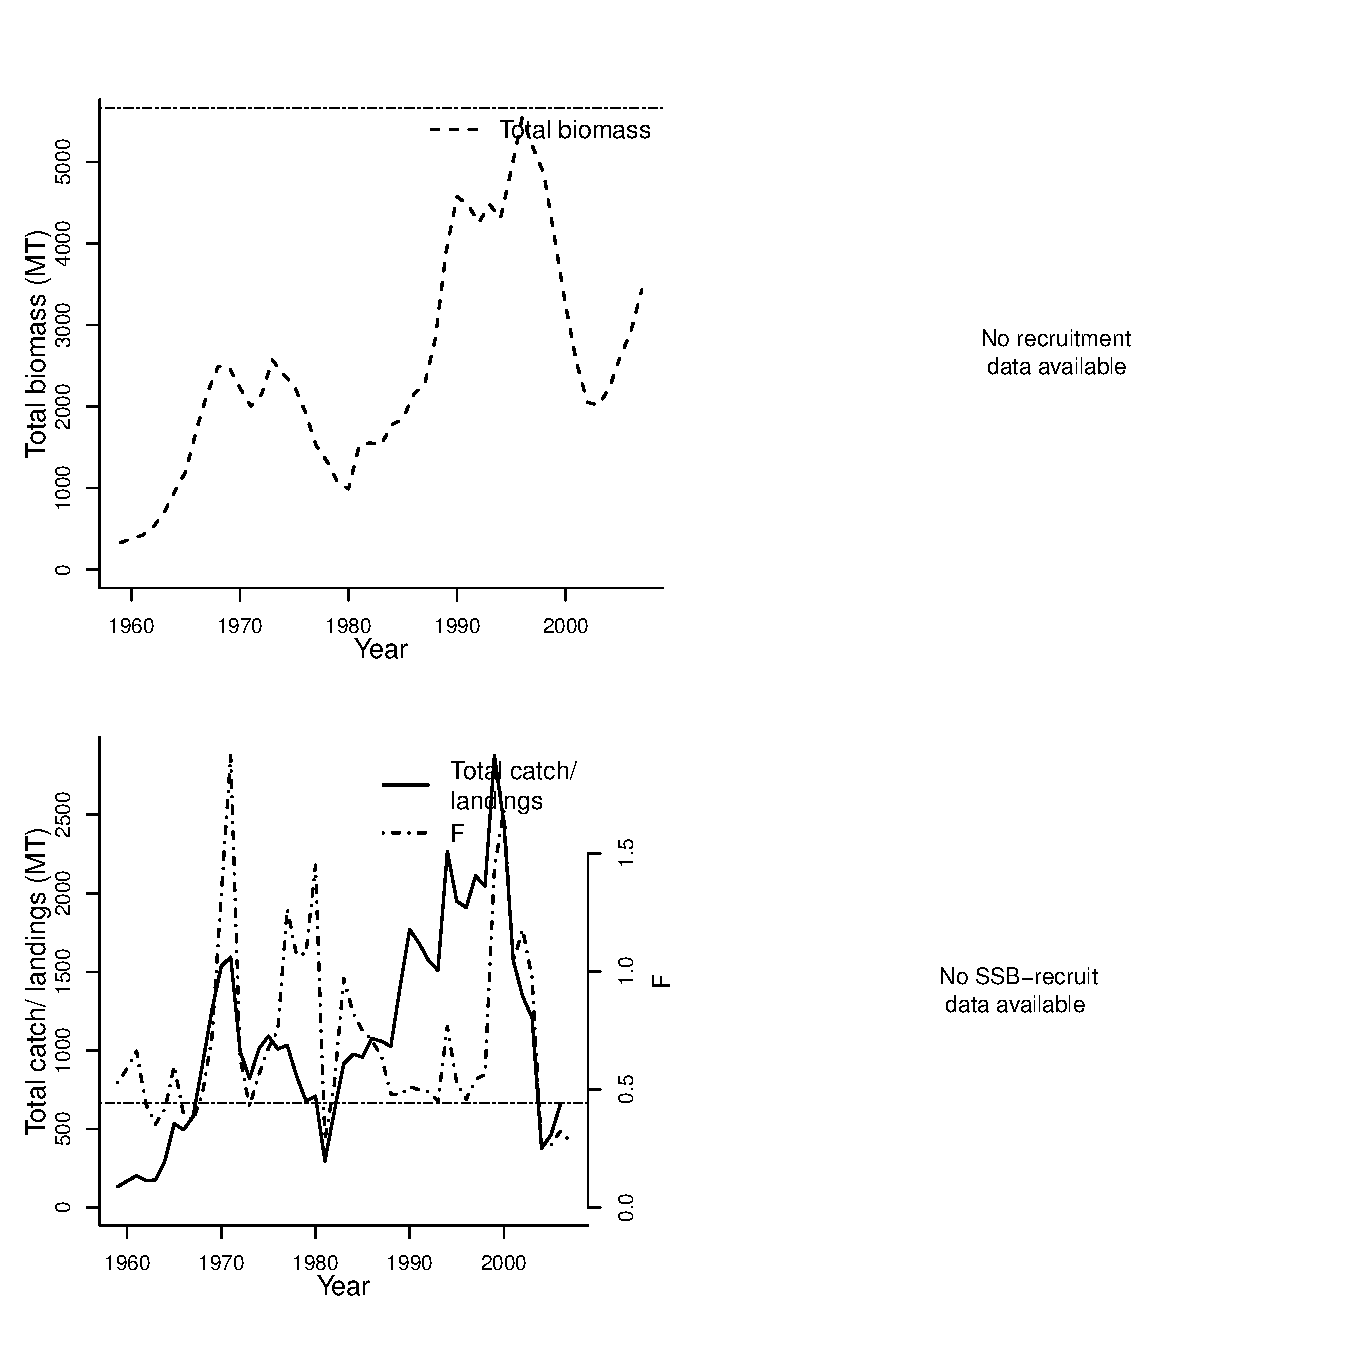
\includegraphics[scale=0.65]{../tex/figures/plot-RIDEM-LOBSTERRI-1959-2007-COLLIE.pdf}
\end{center}

\newpage
\section{Gadiformes}\index{Gadiformes}

\subsection{Gadidae}\index{Gadidae}\index{Gadiformes!Gadidae}

\subsubsection{Gadus macrocephalus - Pacific cod}\index{Pacific cod}\index{Gadus macrocephalus}\index{Gadidae!Gadus macrocephalus}
ID: DFO-PAC-PCODHS-1956-2005-COLLIE

Pacific cod Hecate Strait 

stock assessment conducted: Delay difference model 
\begin{center}
\vspace{-0.2cm}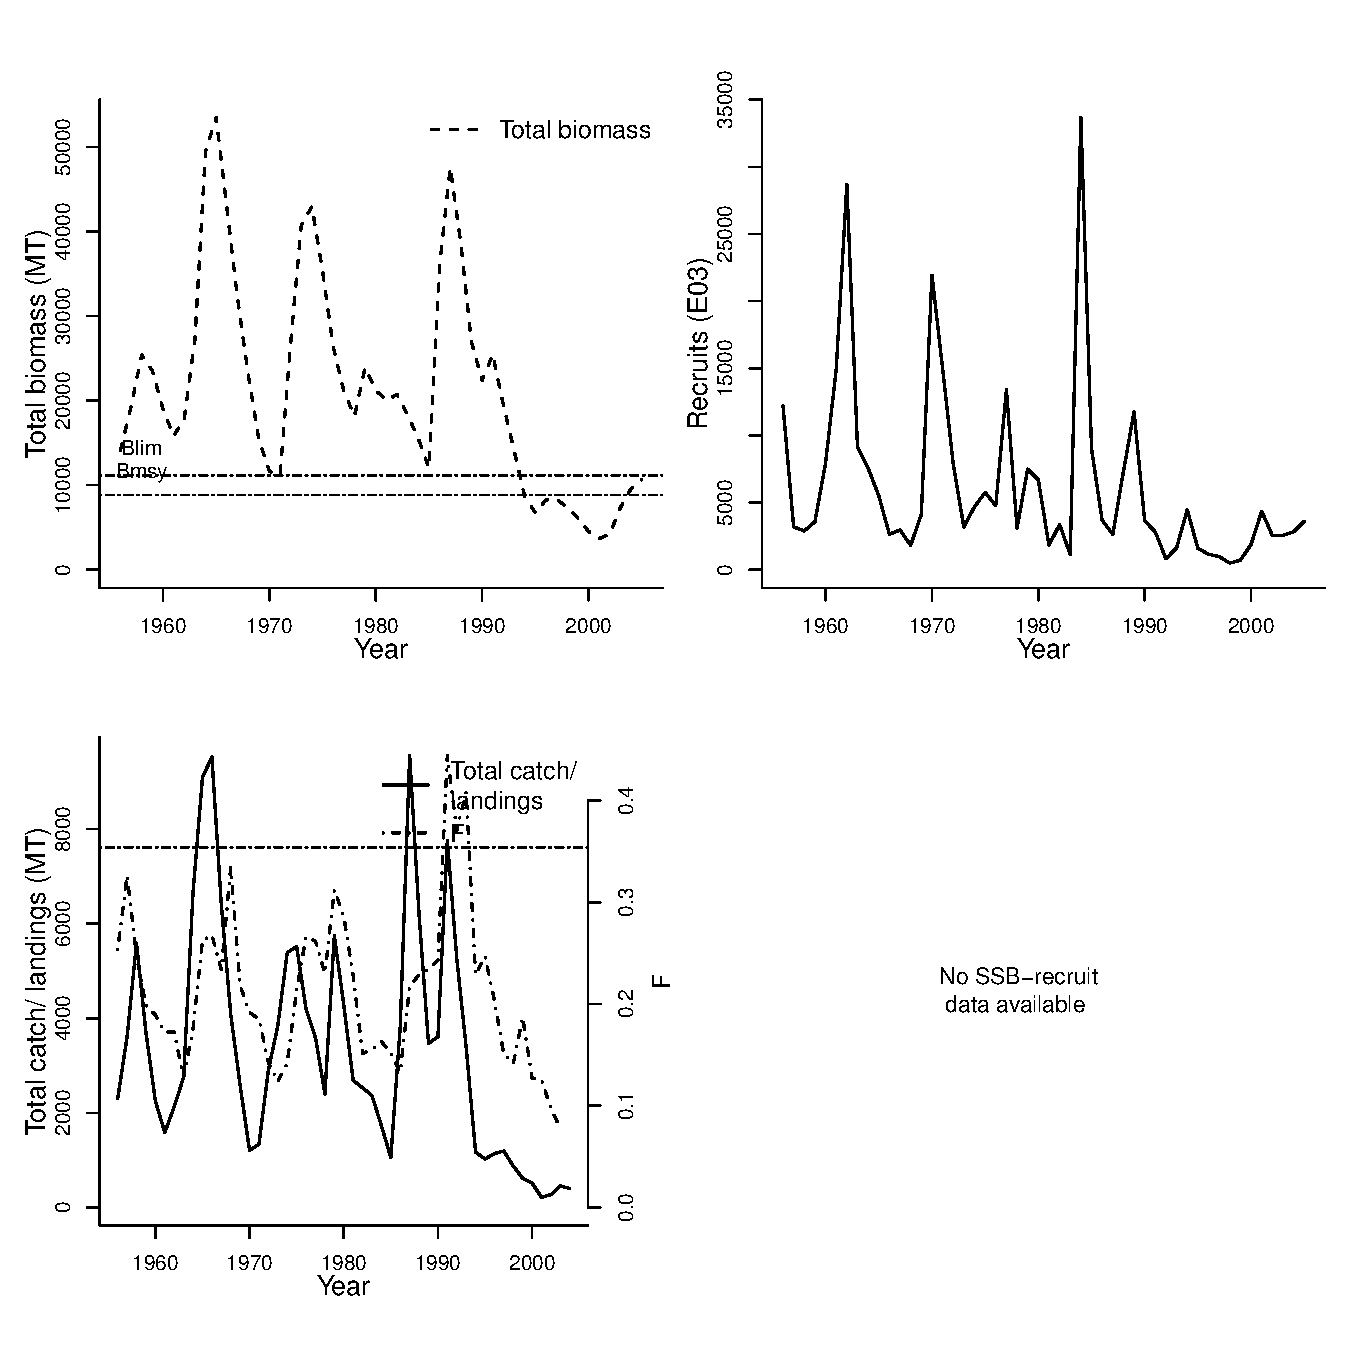
\includegraphics[scale=0.65]{../tex/figures/plot-DFO-PAC-PCODHS-1956-2005-COLLIE.pdf}
\end{center}

\newpage
\subsubsection{Gadus macrocephalus - Pacific cod}\index{Pacific cod}\index{Gadus macrocephalus}\index{Gadidae!Gadus macrocephalus}
ID: DFO-PAC-PCODWCVANI-1956-2002-COLLIE

Pacific cod West Coast of Vancouver Island 

stock assessment conducted: Delay difference model 
\begin{center}
\vspace{-0.2cm}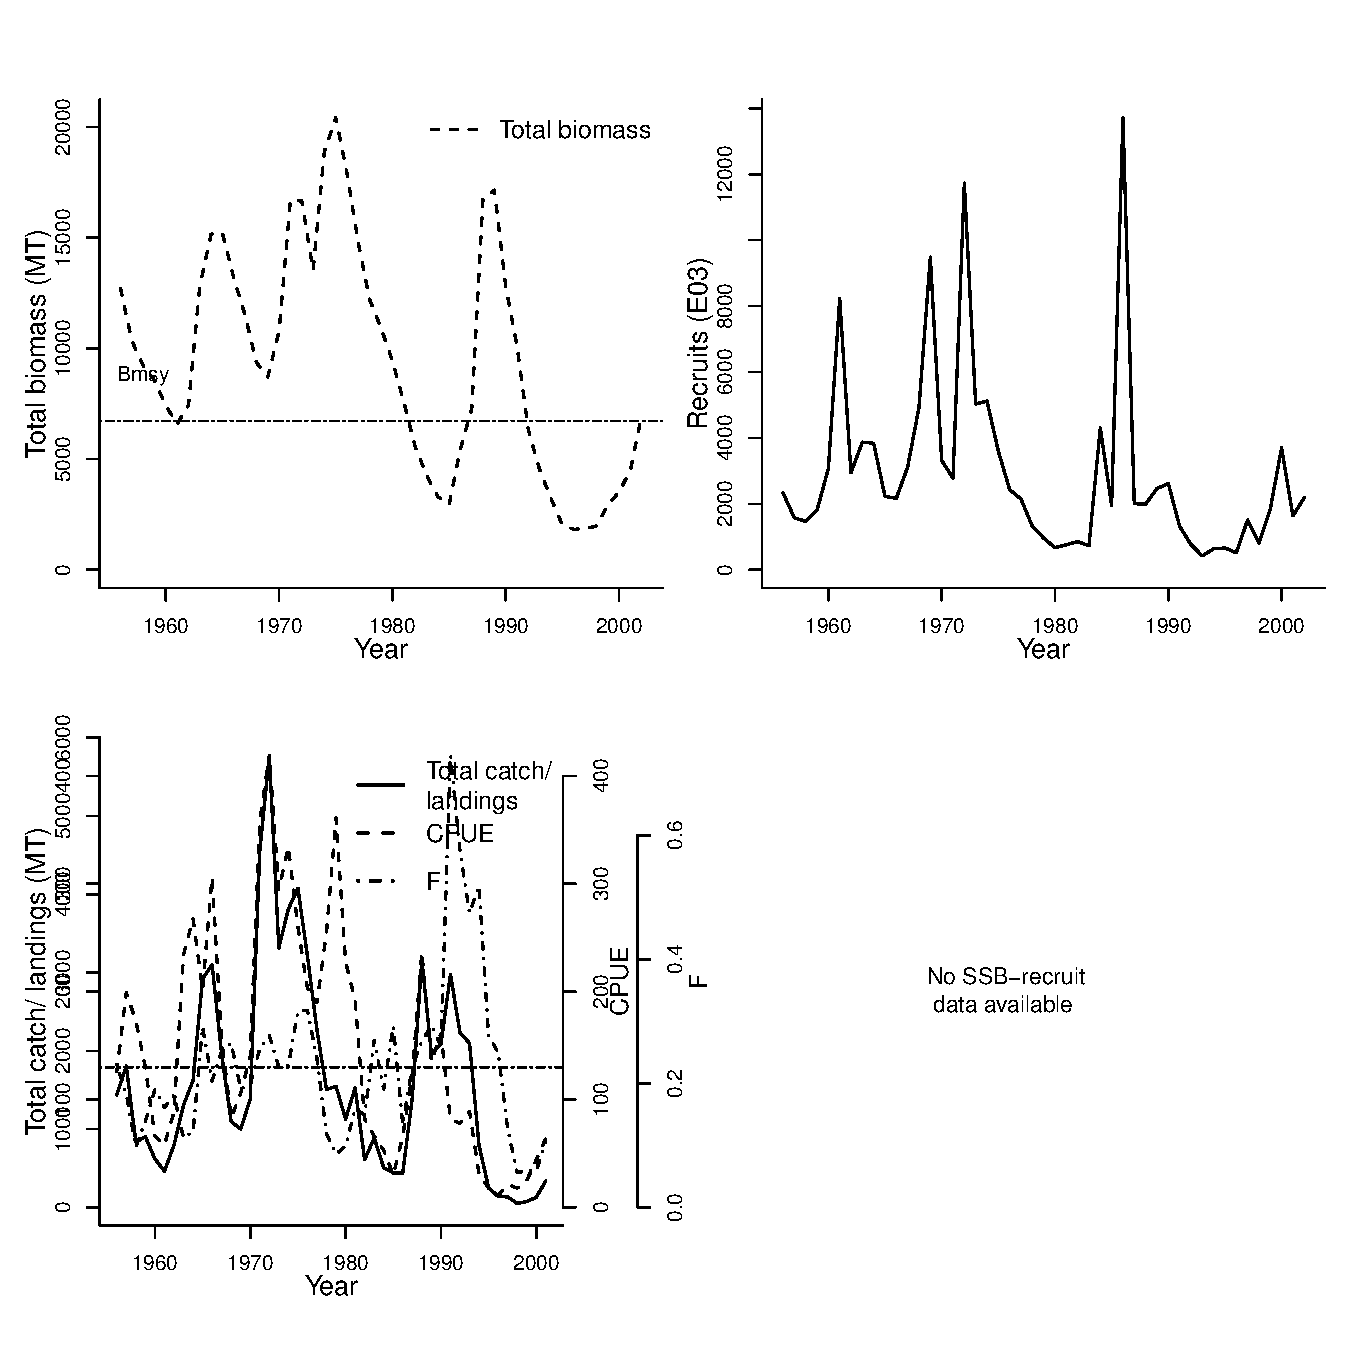
\includegraphics[scale=0.65]{../tex/figures/plot-DFO-PAC-PCODWCVANI-1956-2002-COLLIE.pdf}
\end{center}

\newpage
\subsubsection{Gadus morhua - Atlantic cod}\index{Atlantic cod}\index{Gadus morhua}\index{Gadidae!Gadus morhua}
ID: WGBFAS-CODBA2224-1969-2007-JENNINGS

Atlantic cod Baltic Areas 22 and 24 

stock assessment conducted: Extended Survivor Analysis 
\begin{center}
\vspace{-0.2cm}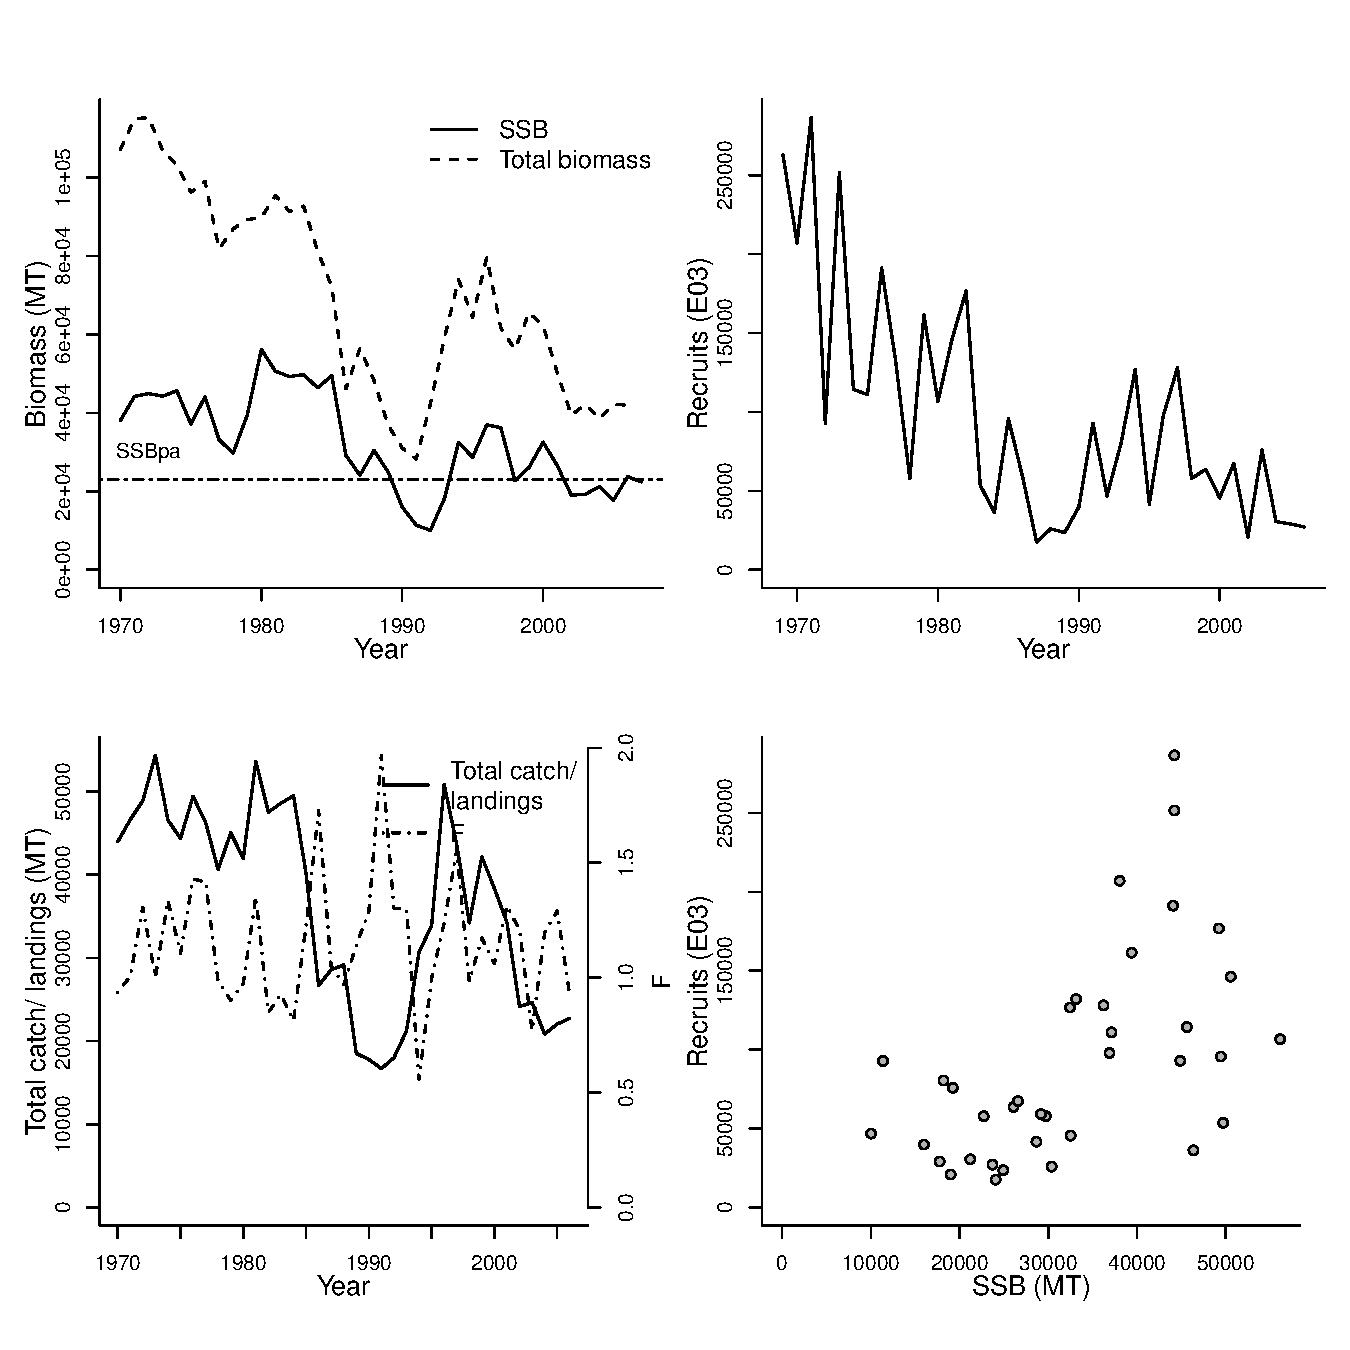
\includegraphics[scale=0.65]{../tex/figures/plot-WGBFAS-CODBA2224-1969-2007-JENNINGS.pdf}
\end{center}

\newpage
\subsubsection{Gadus morhua - Atlantic cod}\index{Atlantic cod}\index{Gadus morhua}\index{Gadidae!Gadus morhua}
ID: WGBFAS-CODBA2532-1964-2007-JENNINGS

Atlantic cod Baltic Areas 25-32 

stock assessment conducted: Extended Survivor Analysis 
\begin{center}
\vspace{-0.2cm}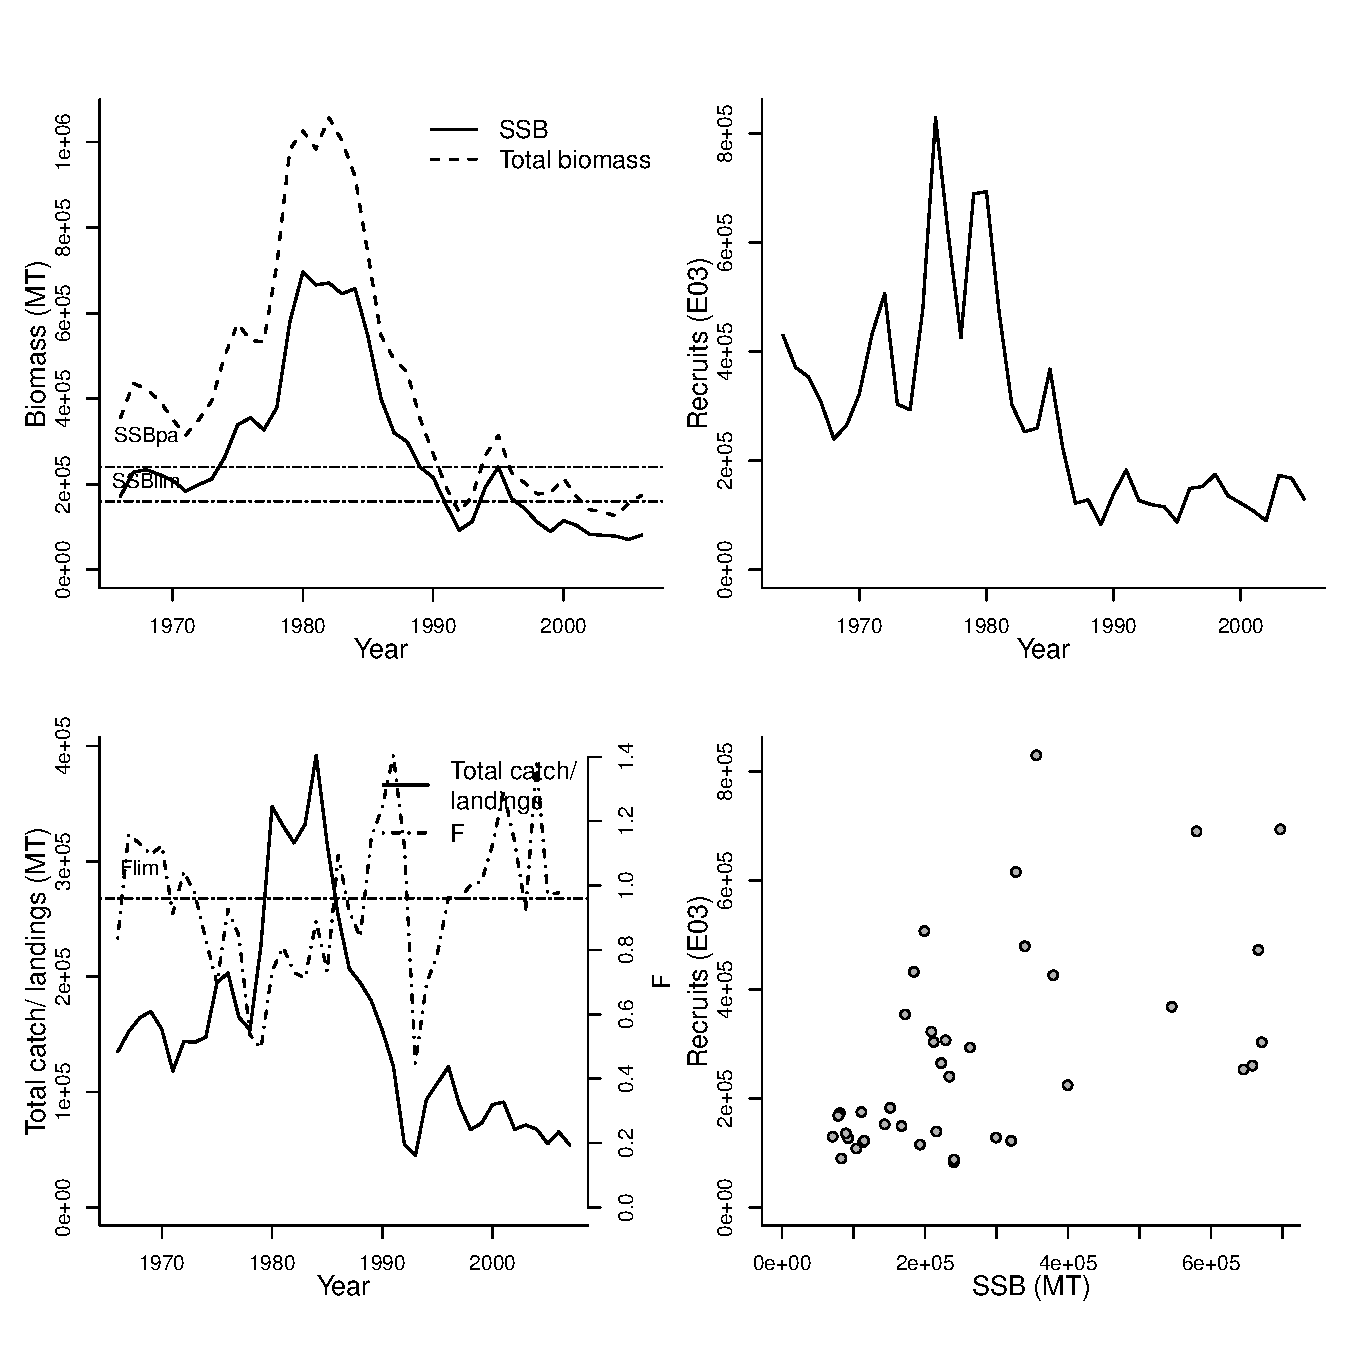
\includegraphics[scale=0.65]{../tex/figures/plot-WGBFAS-CODBA2532-1964-2007-JENNINGS.pdf}
\end{center}

\newpage
\subsubsection{Melanogrammus aeglefinus - Haddock}\index{Haddock}\index{Melanogrammus aeglefinus}\index{Gadidae!Melanogrammus aeglefinus}
ID: WGSSDS-HADVIIb-k-1993-2006-JENNINGS

Haddock ICES VIIb-k 

stock assessment conducted: Extended Survivor Analysis 
\begin{center}
\vspace{-0.2cm}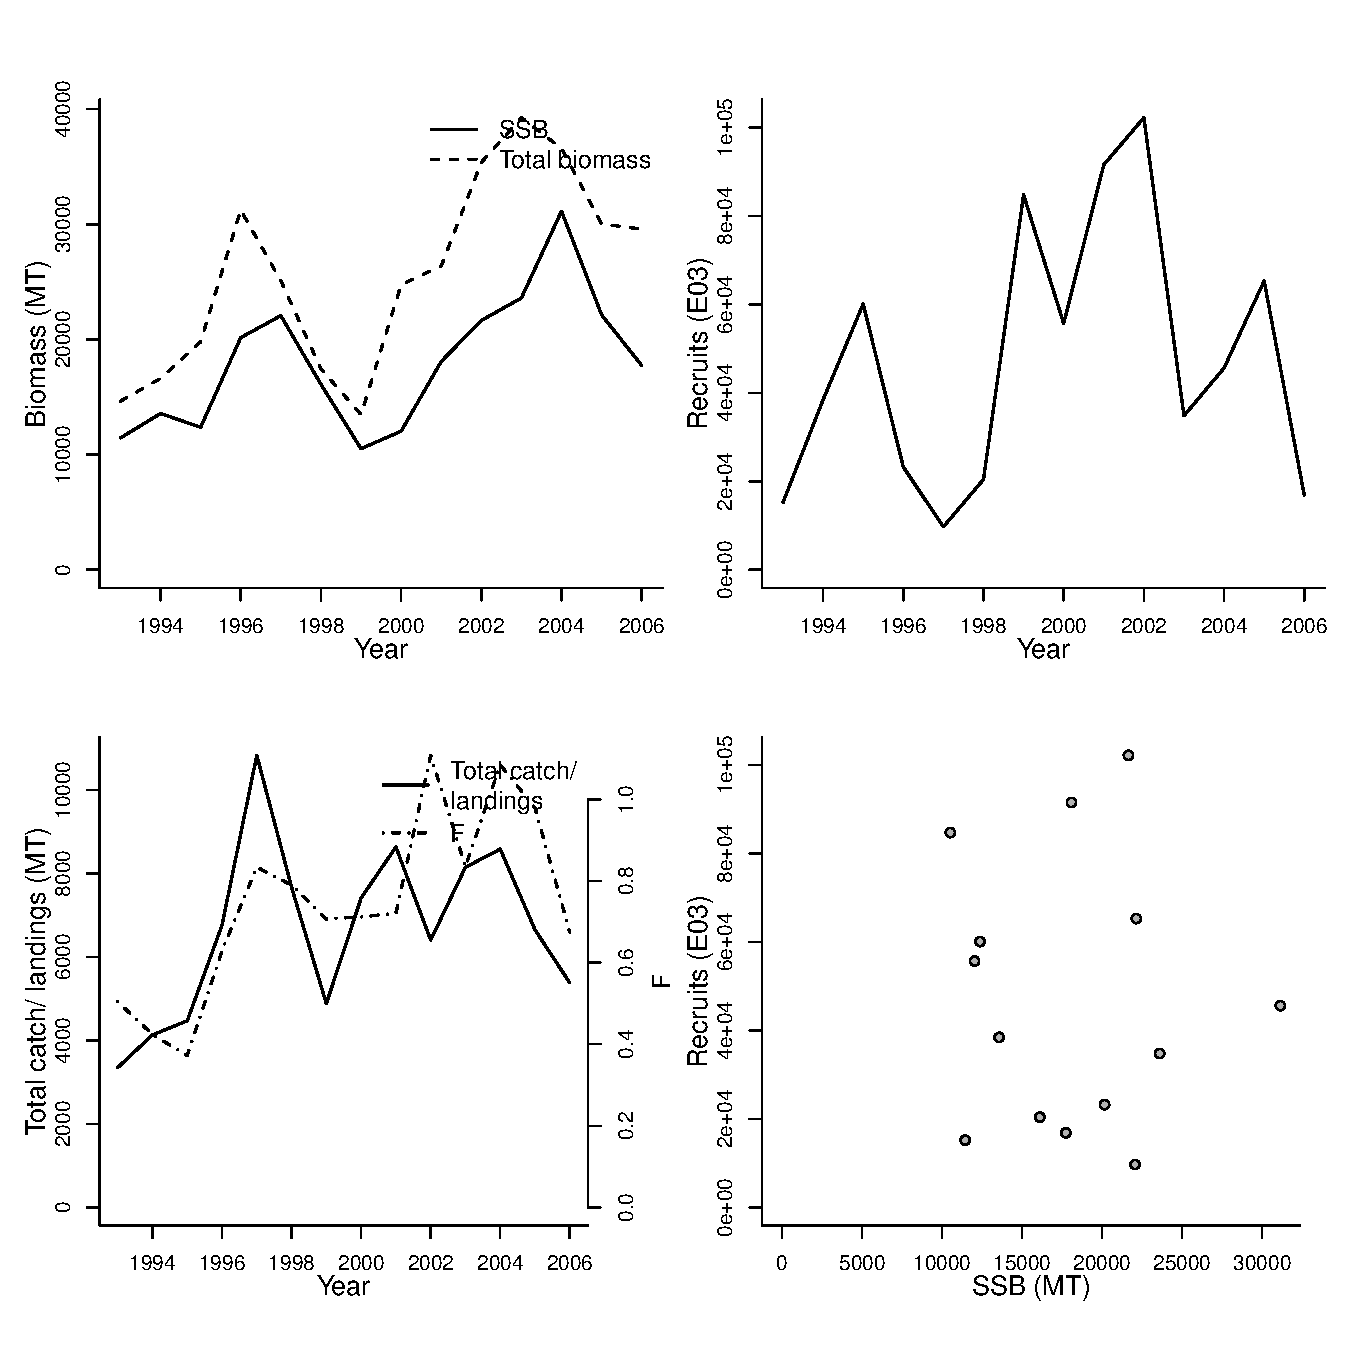
\includegraphics[scale=0.65]{../tex/figures/plot-WGSSDS-HADVIIb-k-1993-2006-JENNINGS.pdf}
\end{center}

\newpage
\subsubsection{Melanogrammus aeglefinus - Haddock}\index{Haddock}\index{Melanogrammus aeglefinus}\index{Gadidae!Melanogrammus aeglefinus}
ID: WGNSSK-HADROCK-1990-2007-JENNINGS

Haddock Rockall Bank 

stock assessment conducted: Extended Survivor Analysis 
\begin{center}
\vspace{-0.2cm}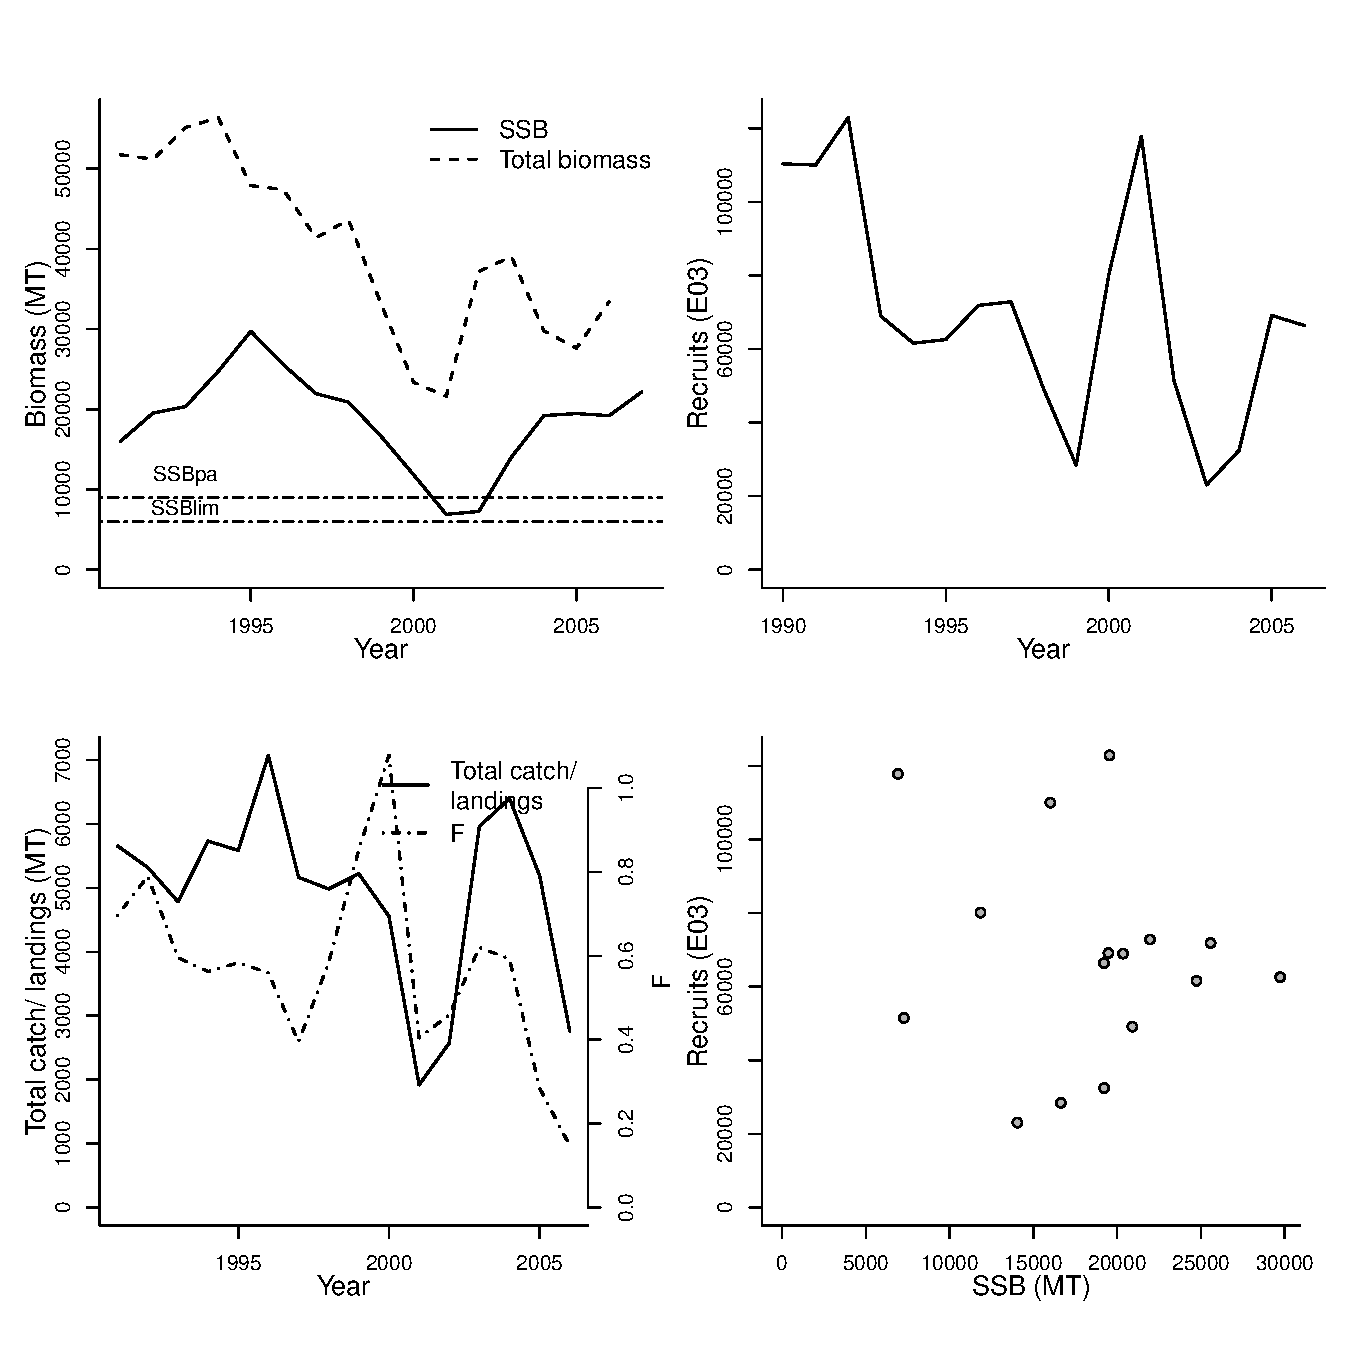
\includegraphics[scale=0.65]{../tex/figures/plot-WGNSSK-HADROCK-1990-2007-JENNINGS.pdf}
\end{center}

\newpage
\subsubsection{Merlangius merlangus - Whiting}\index{Whiting}\index{Merlangius merlangus}\index{Gadidae!Merlangius merlangus}
ID: WGSSDS-WHITVIIek-1982-2007-JENNINGS

Whiting ICES VIIe-k 

stock assessment conducted: Extended Survivor Analysis 
\begin{center}
\vspace{-0.2cm}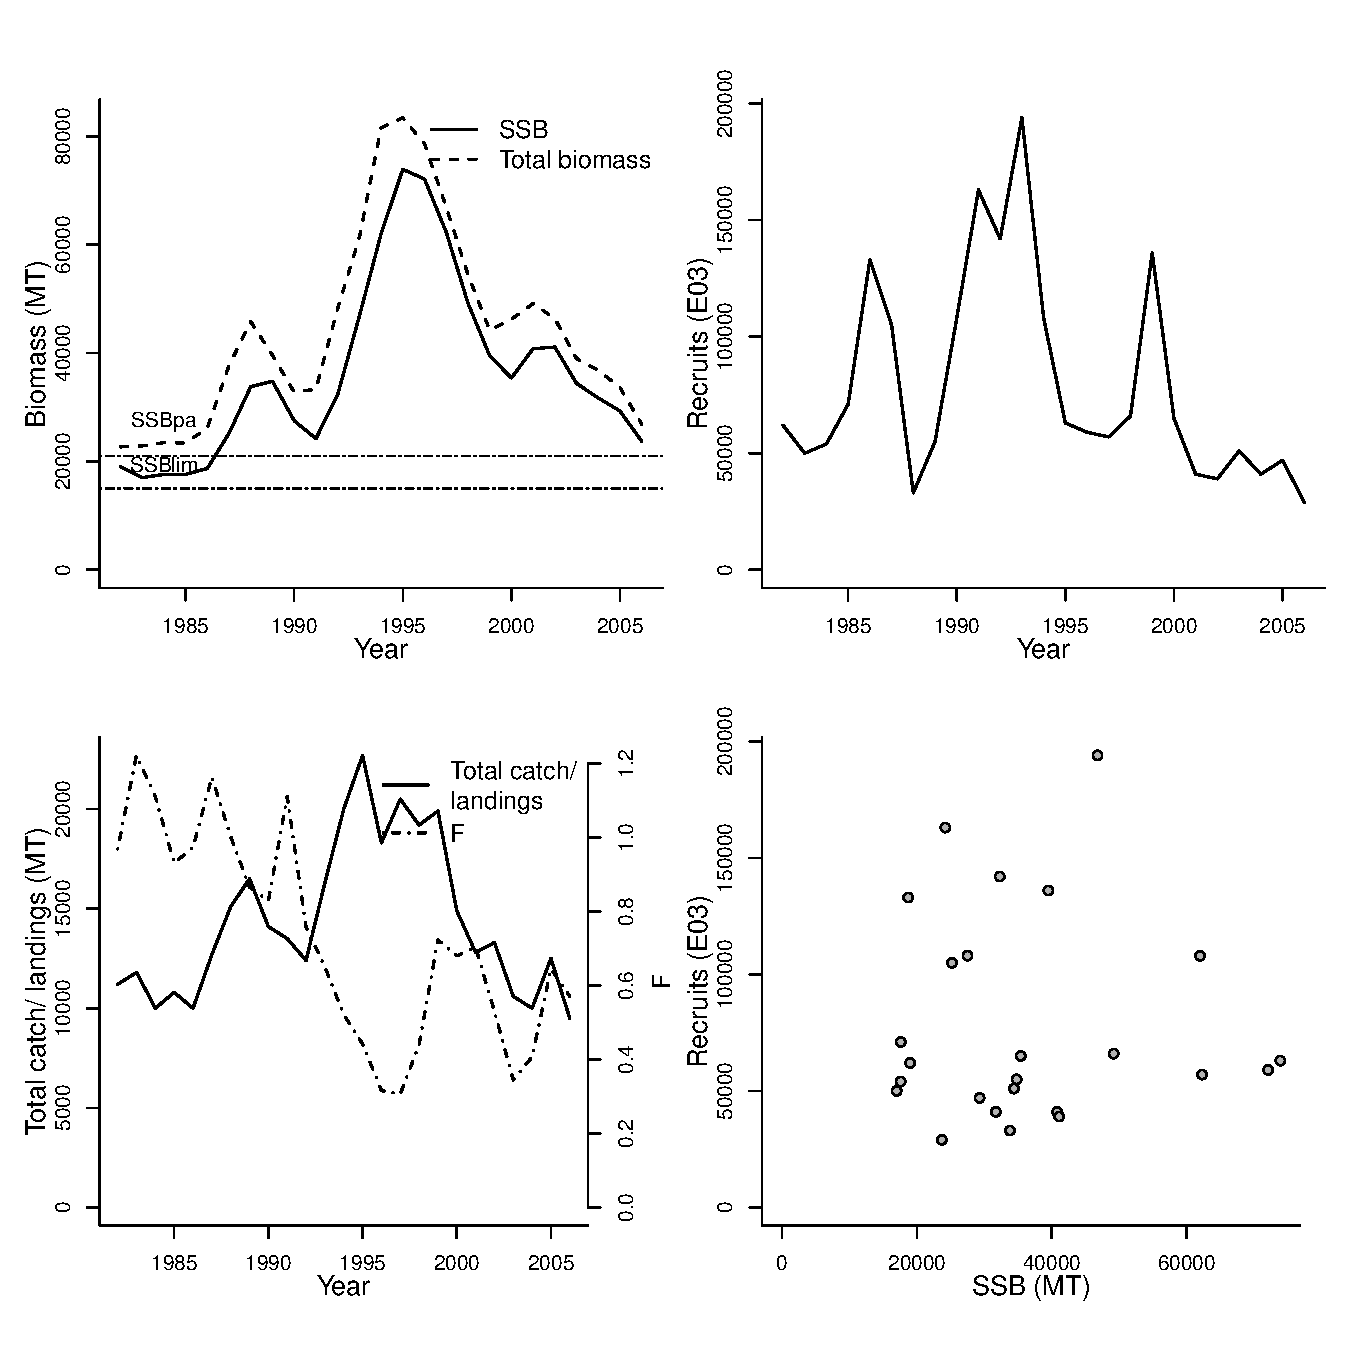
\includegraphics[scale=0.65]{../tex/figures/plot-WGSSDS-WHITVIIek-1982-2007-JENNINGS.pdf}
\end{center}

\newpage
\subsubsection{Micromesistius australis - Southern blue whiting}\index{Southern blue whiting}\index{Micromesistius australis}\index{Gadidae!Micromesistius australis}
ID: INIDEP-SBWHITARGS-1985-2007-Parma

 Southern blue whiting Southern Argentina 

stock assessment conducted: Virtual Population Analysis 
\begin{center}
\vspace{-0.2cm}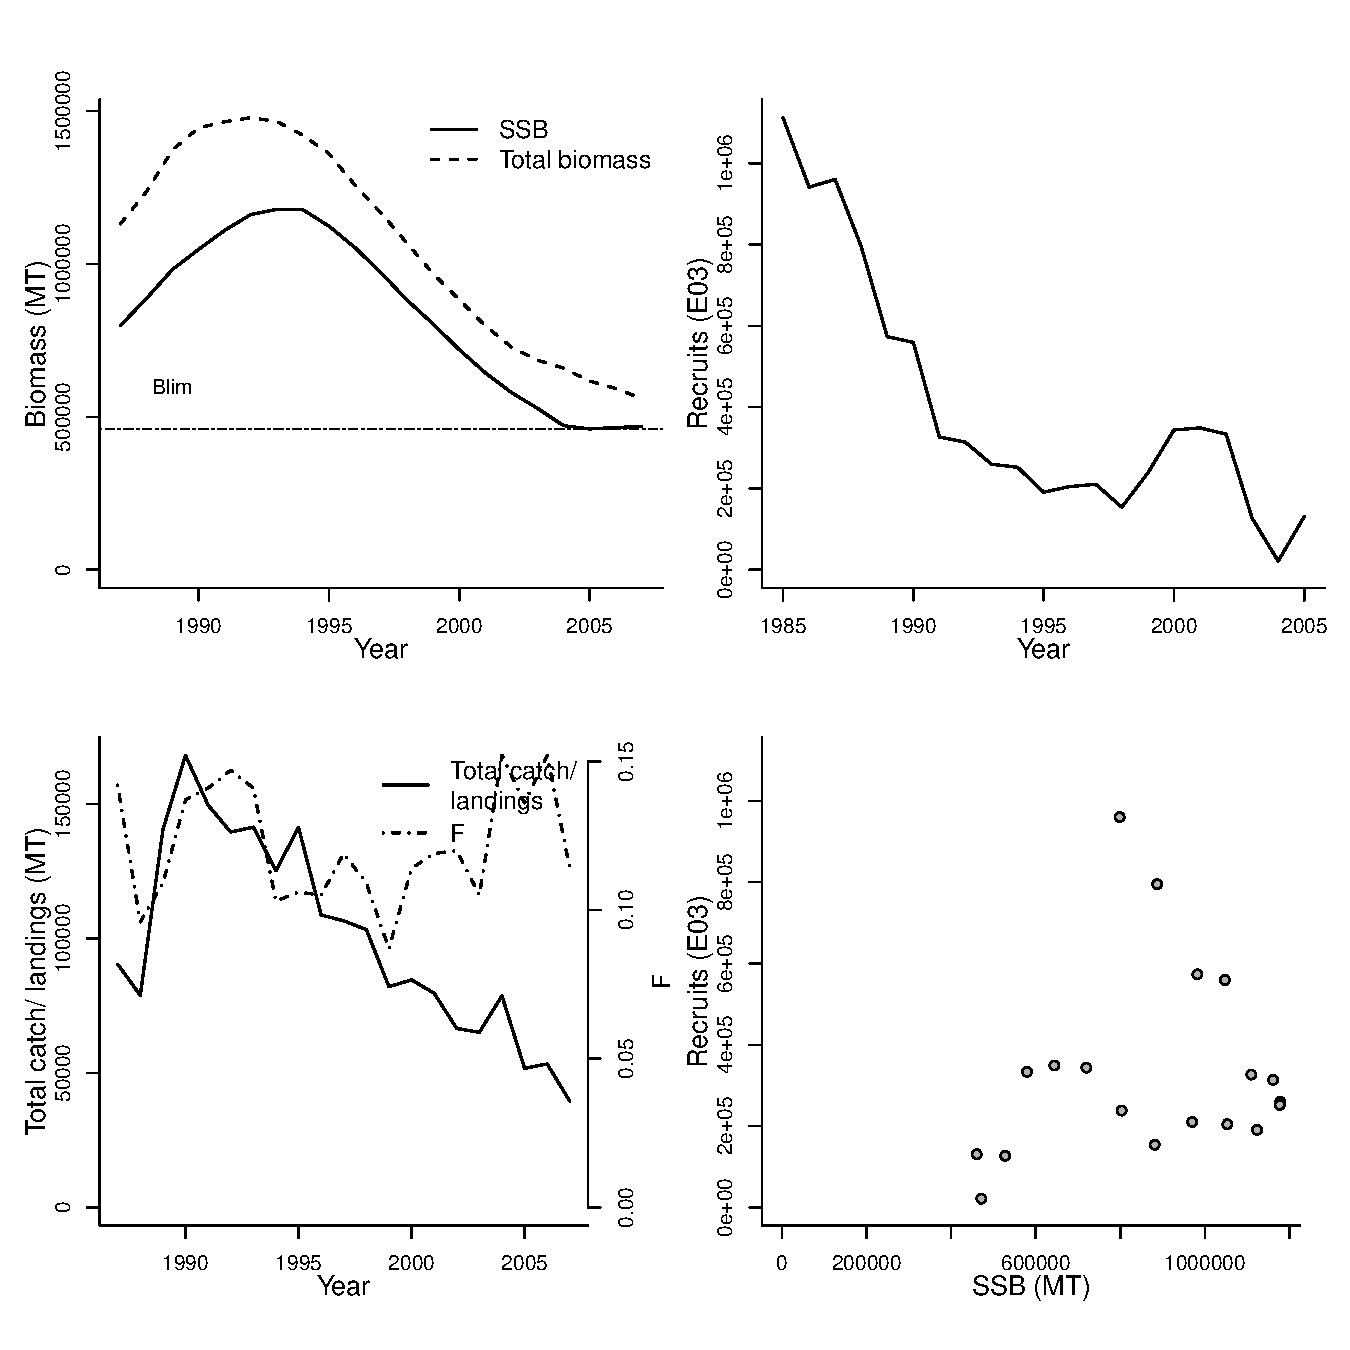
\includegraphics[scale=0.65]{../tex/figures/plot-INIDEP-SBWHITARGS-1985-2007-Parma.pdf}
\end{center}

\newpage
\subsubsection{Micromesistius poutassou - Blue whiting}\index{Blue whiting}\index{Micromesistius poutassou}\index{Gadidae!Micromesistius poutassou}
ID: WGNPBW-BWHITNEA-1980-2007-JENNINGS

Whiting Northeast Atlantic 

stock assessment conducted: Stochastic Multi-species (SMS) model 
\begin{center}
\vspace{-0.2cm}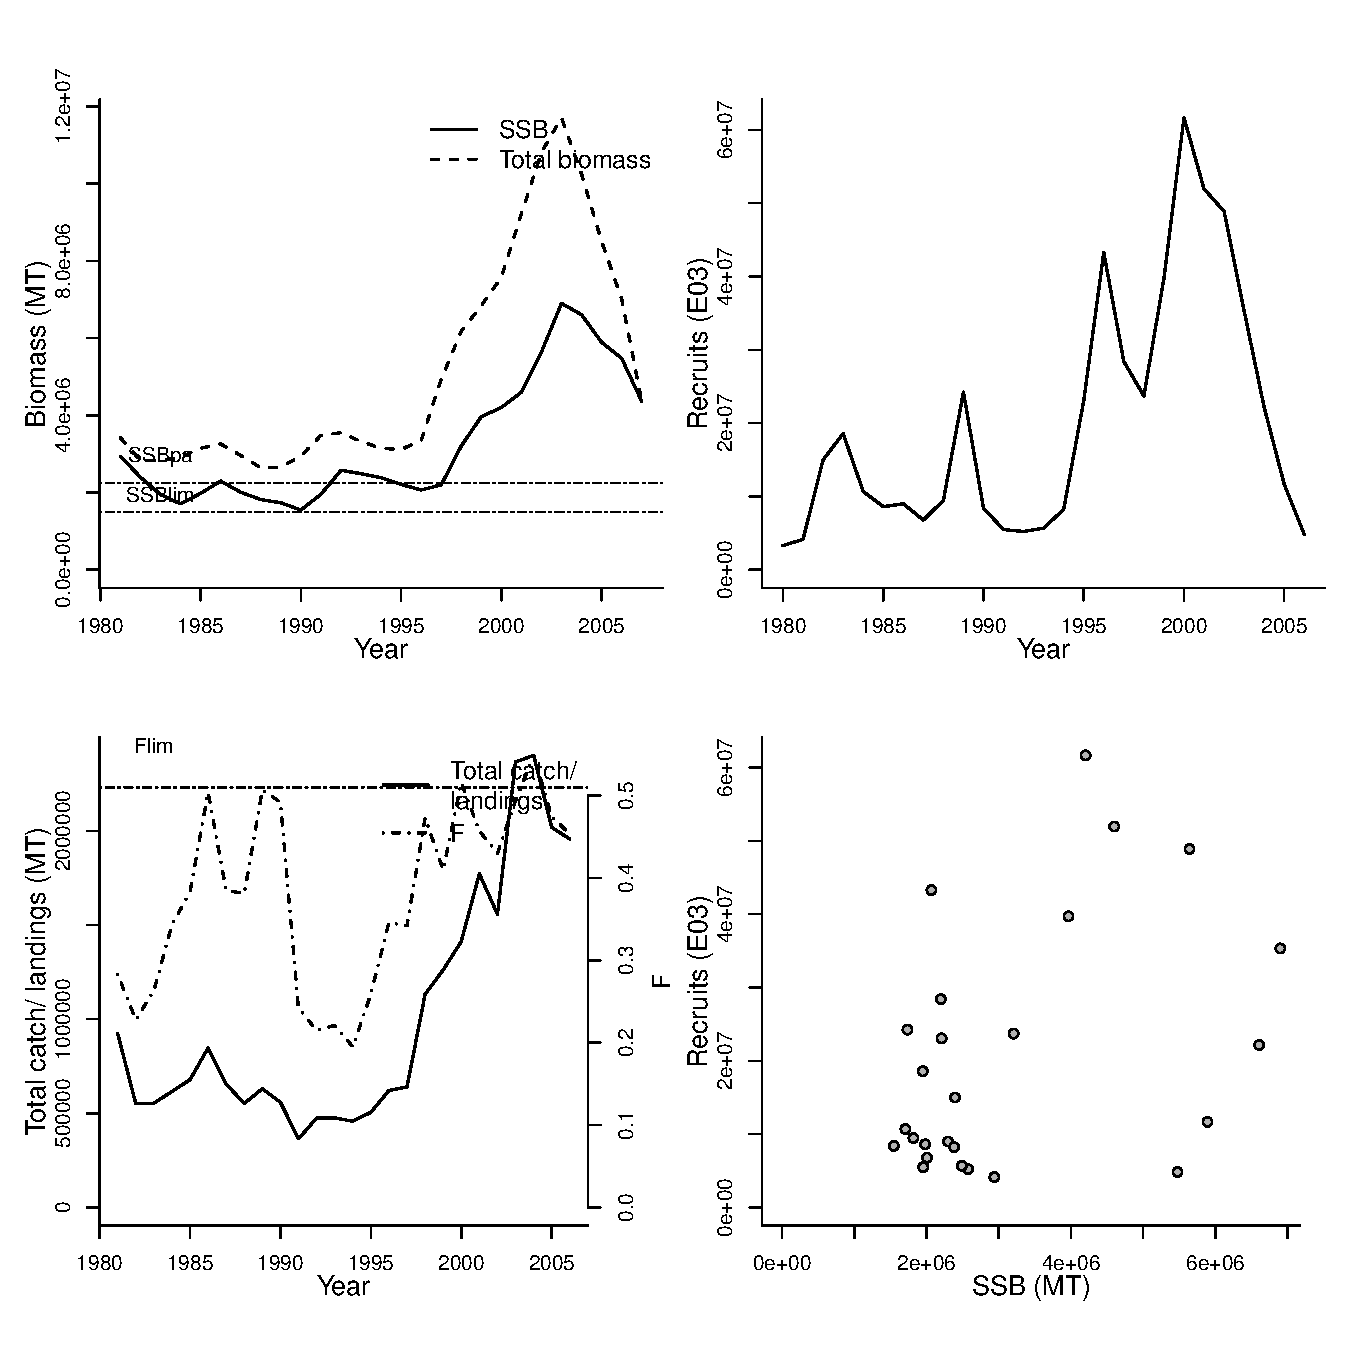
\includegraphics[scale=0.65]{../tex/figures/plot-WGNPBW-BWHITNEA-1980-2007-JENNINGS.pdf}
\end{center}

\newpage
\subsection{Merlucciidae}\index{Merlucciidae}\index{Gadiformes!Merlucciidae}

\subsubsection{Macruronus magellanicus - Patagonian grenadier}\index{Patagonian grenadier}\index{Macruronus magellanicus}\index{Merlucciidae!Macruronus magellanicus}
ID: INIDEP-PATGRENADIERSARG-1983-2006-Parma

Patagonian grenadier Southern Argentina 

stock assessment conducted: Virtual Population Analysis 
\begin{center}
\vspace{-0.2cm}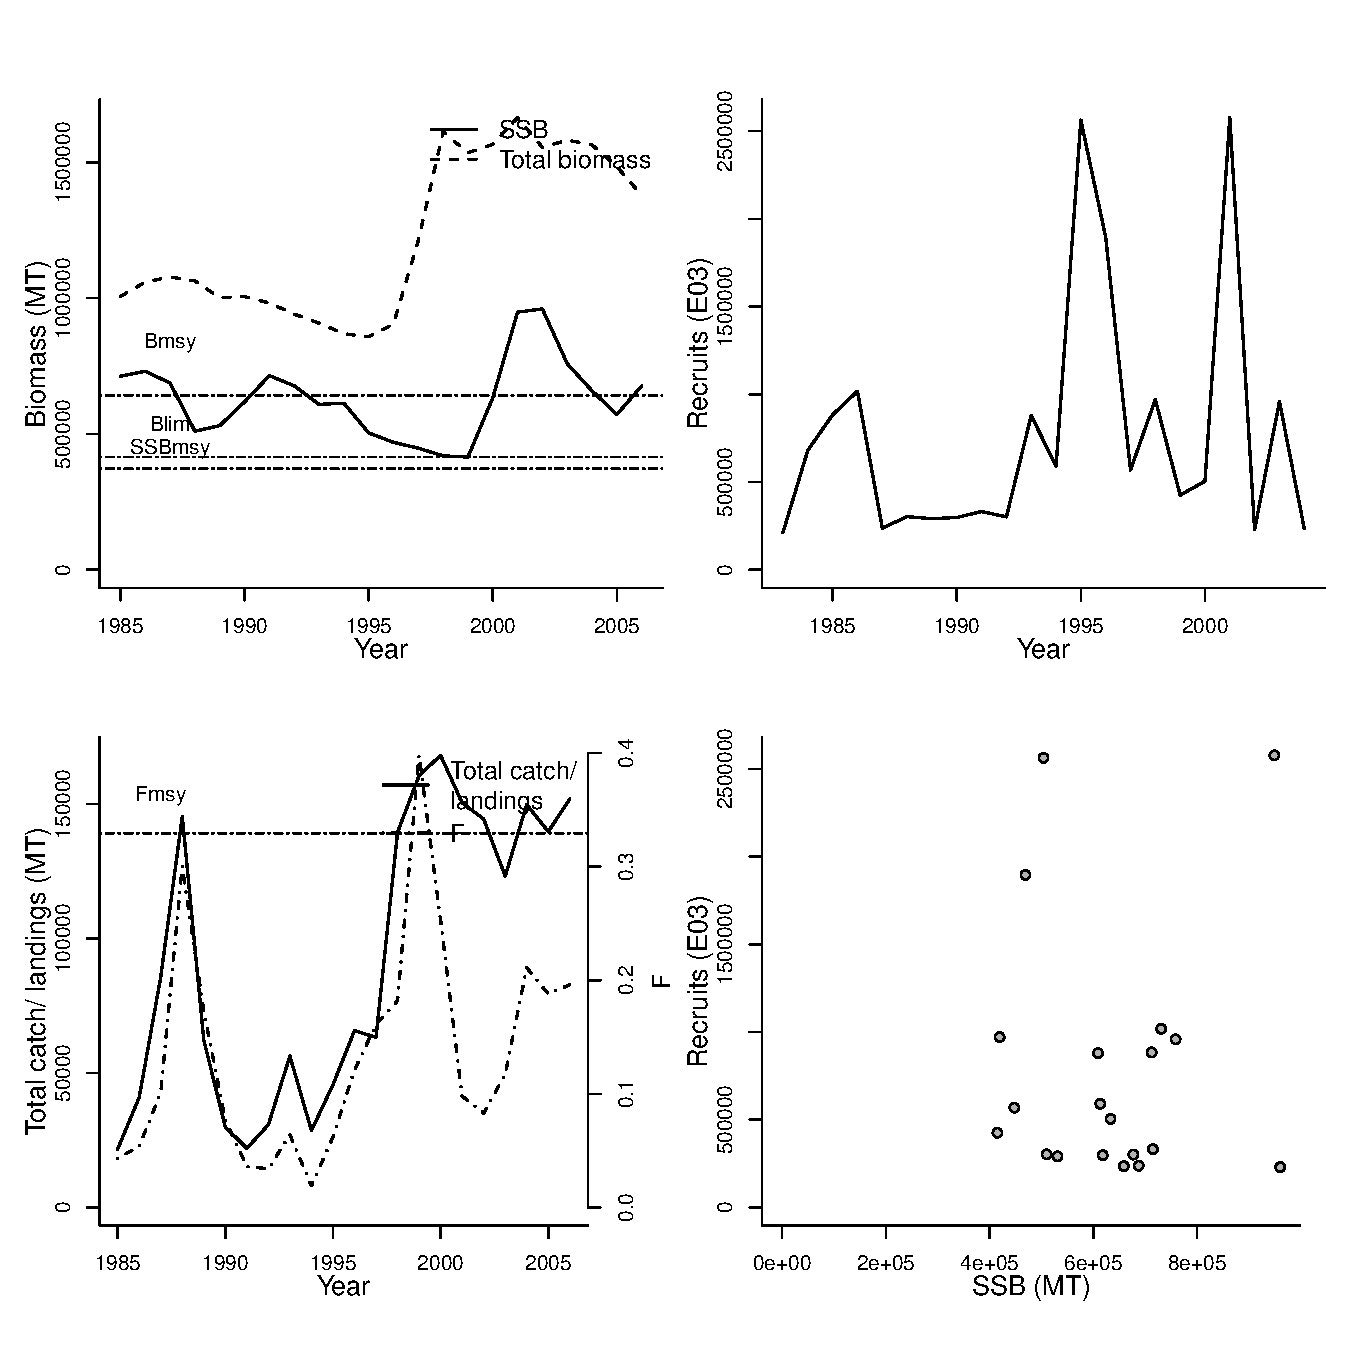
\includegraphics[scale=0.65]{../tex/figures/plot-INIDEP-PATGRENADIERSARG-1983-2006-Parma.pdf}
\end{center}

\newpage
\subsubsection{Merluccius hubbsi - Argentine hake}\index{Argentine hake}\index{Merluccius hubbsi}\index{Merlucciidae!Merluccius hubbsi}
ID: INIDEP-ARGHAKENARG-1985-2007-Parma

Argentine hake Northern Argentina 

stock assessment conducted: Virtual Population Analysis 
\begin{center}
\vspace{-0.2cm}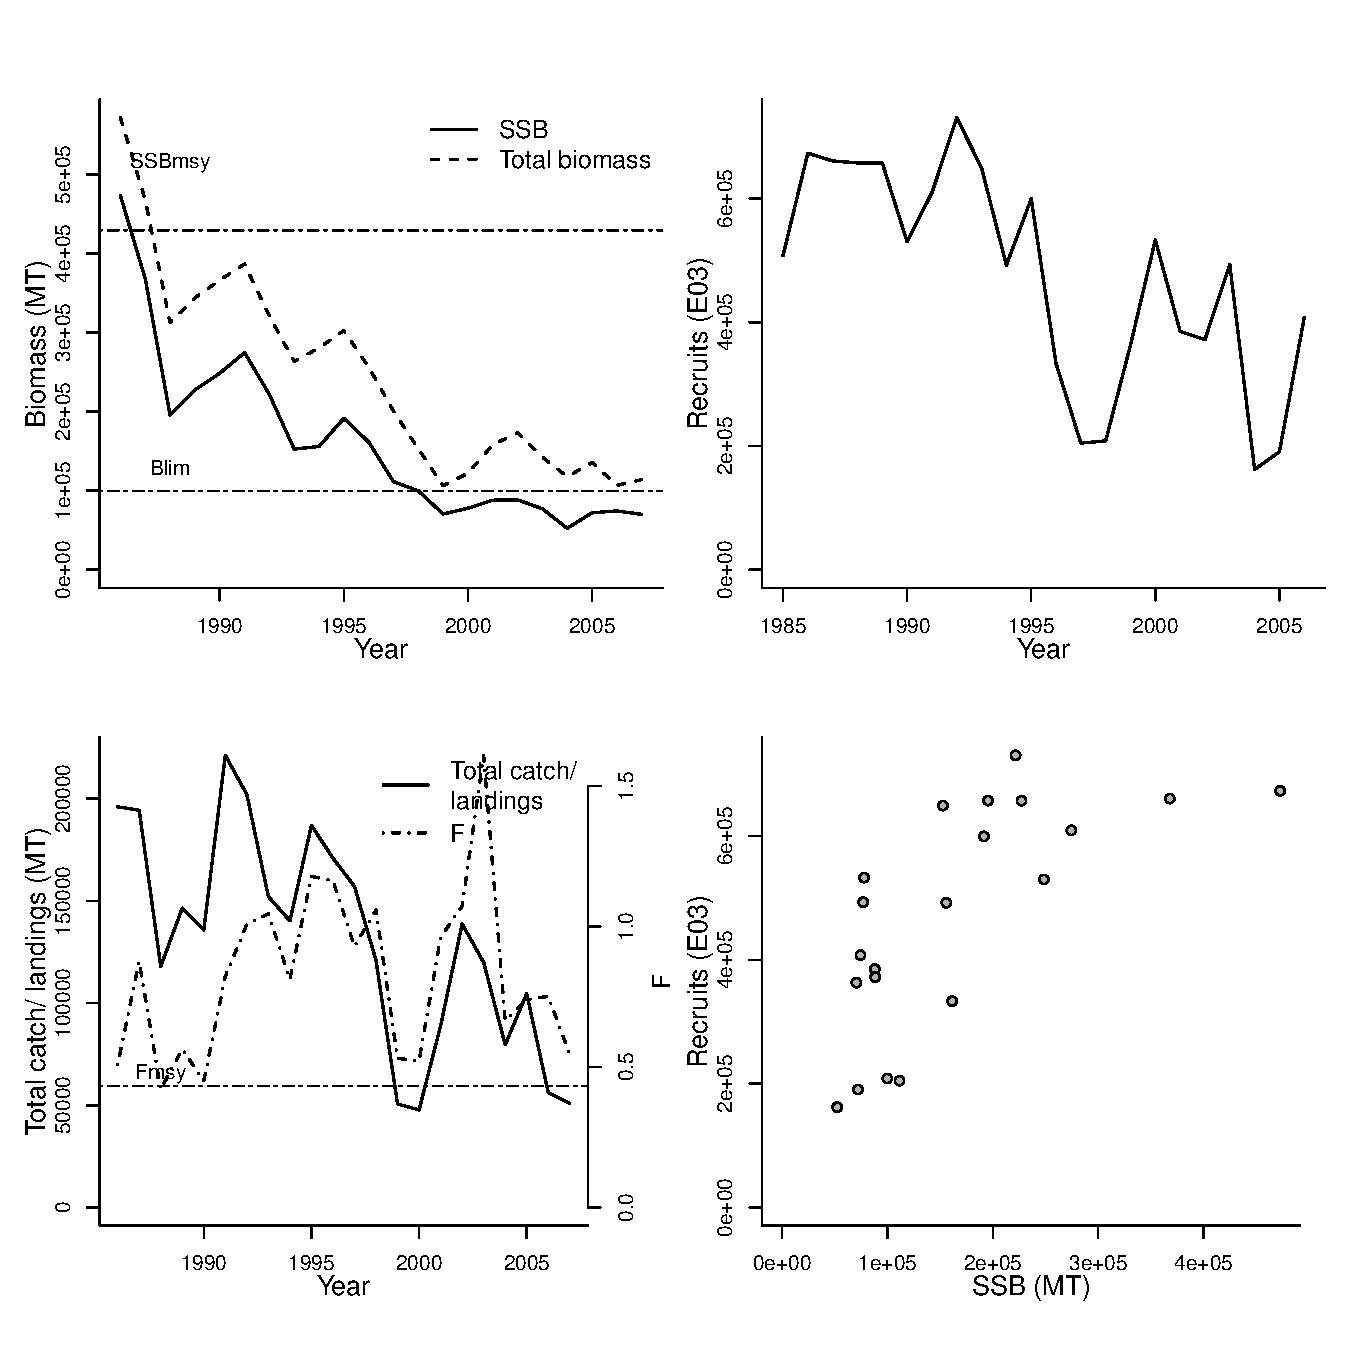
\includegraphics[scale=0.65]{../tex/figures/plot-INIDEP-ARGHAKENARG-1985-2007-Parma.pdf}
\end{center}

\newpage
\subsubsection{Merluccius hubbsi - Argentine hake}\index{Argentine hake}\index{Merluccius hubbsi}\index{Merlucciidae!Merluccius hubbsi}
ID: INIDEP-ARGHAKESARG-1985-2007-Parma

Argentine hake Southern Argentina 

stock assessment conducted: Virtual Population Analysis 
\begin{center}
\vspace{-0.2cm}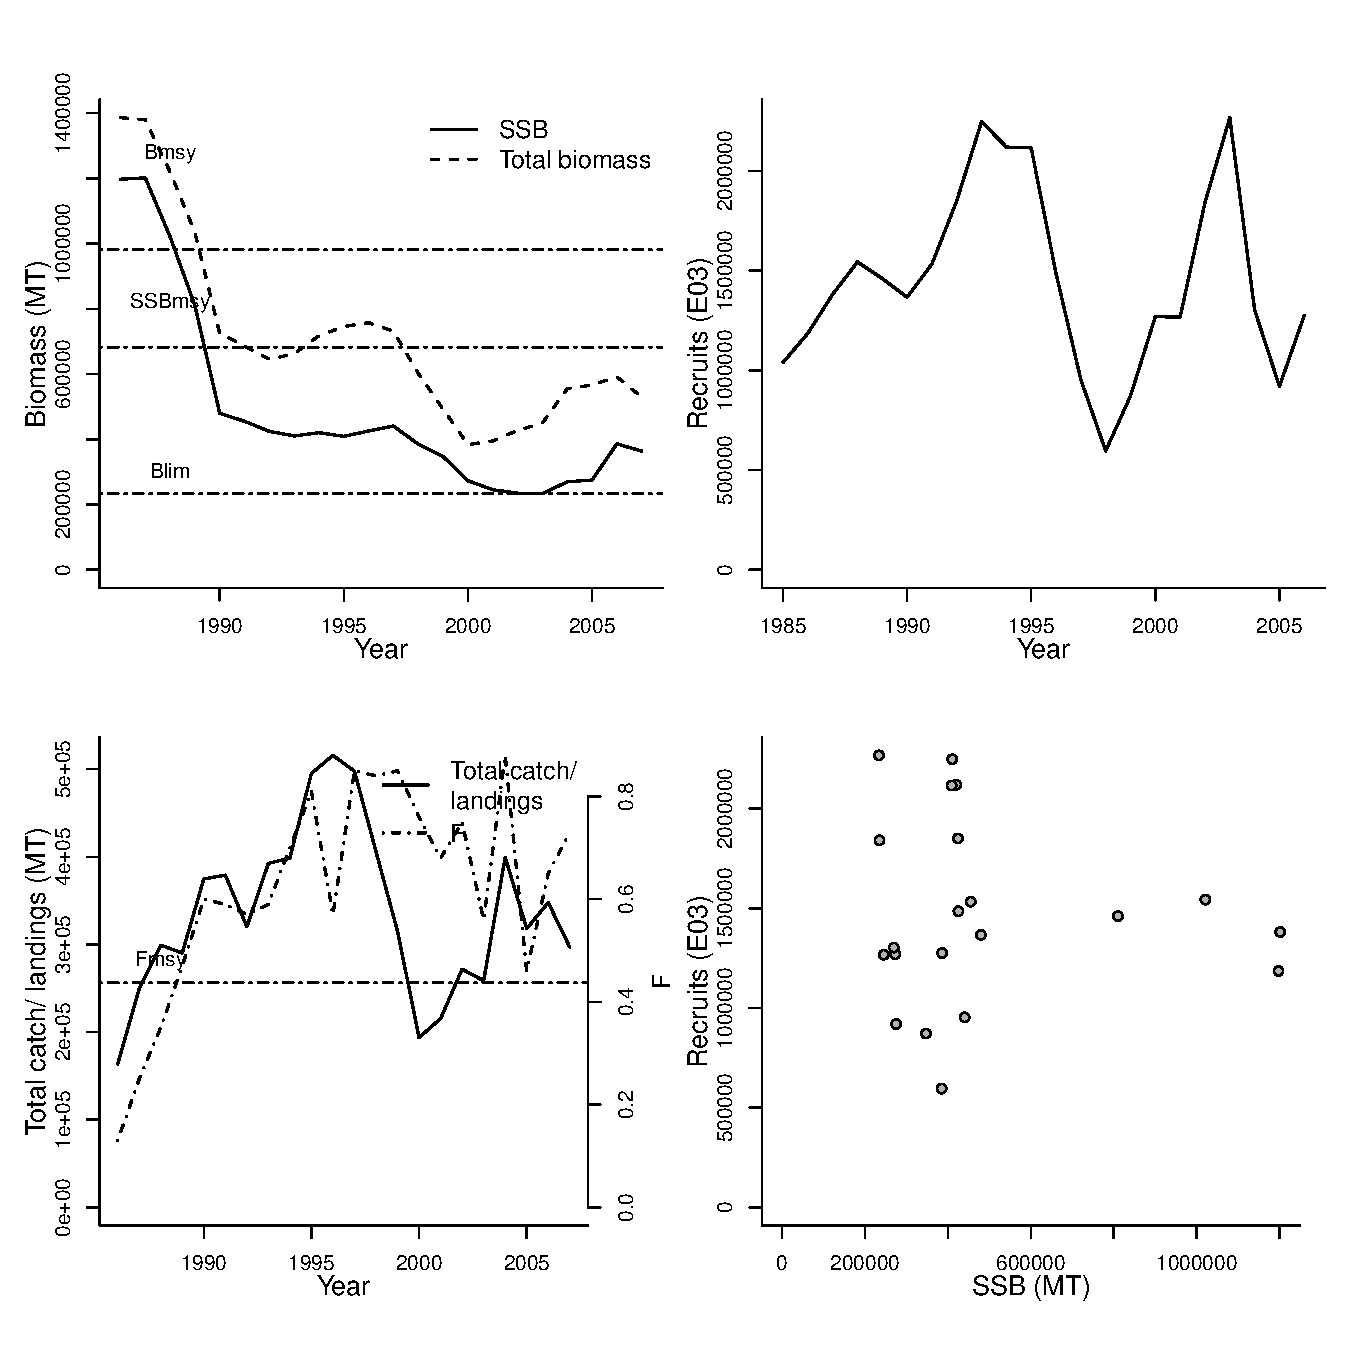
\includegraphics[scale=0.65]{../tex/figures/plot-INIDEP-ARGHAKESARG-1985-2007-Parma.pdf}
\end{center}

\newpage
\subsubsection{Merluccius merluccius - Hake}\index{Hake}\index{Merluccius merluccius}\index{Merlucciidae!Merluccius merluccius}
ID: WGHMM-HAKENRTN-1977-2007-JENNINGS

Hake Northeast Atlantic North 

stock assessment conducted: Extended Survivor Analysis 
\begin{center}
\vspace{-0.2cm}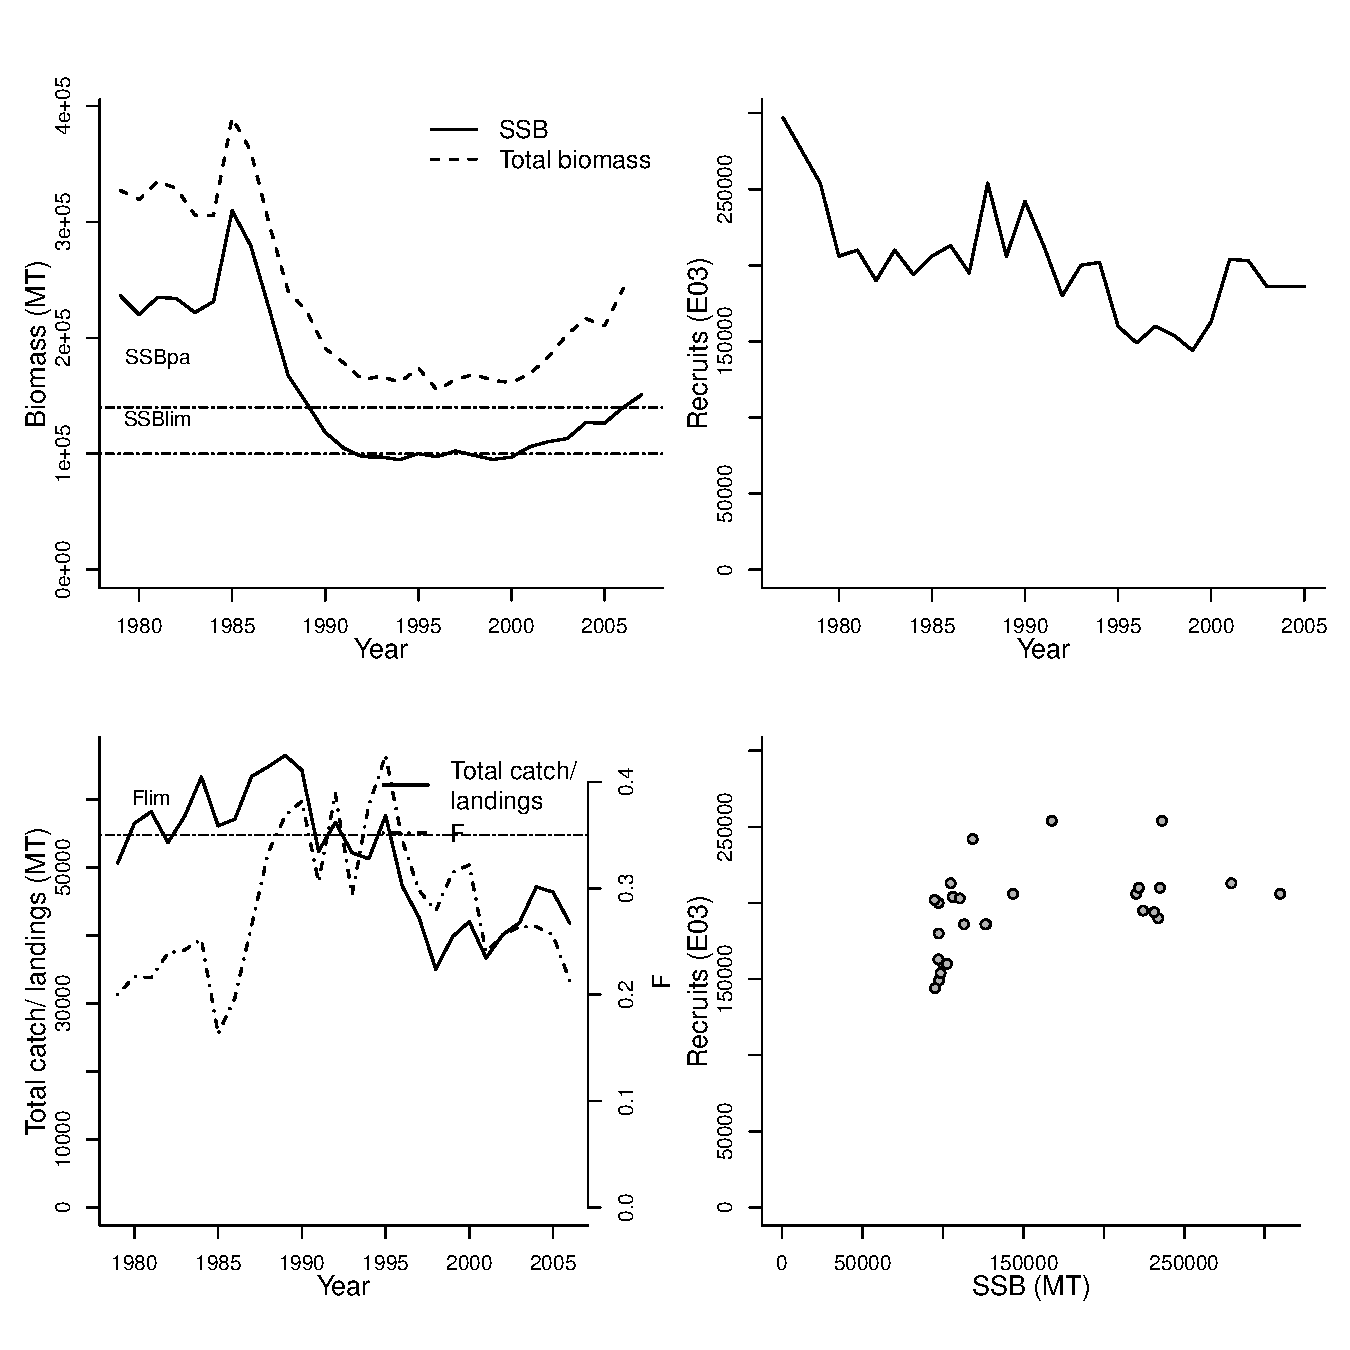
\includegraphics[scale=0.65]{../tex/figures/plot-WGHMM-HAKENRTN-1977-2007-JENNINGS.pdf}
\end{center}

\newpage
\subsubsection{Merluccius merluccius - Hake}\index{Hake}\index{Merluccius merluccius}\index{Merlucciidae!Merluccius merluccius}
ID: WGHMM-HAKESOTH-1982-2007-JENNINGS

Hake Northeast Atlantic South 

stock assessment conducted: Extended Survivor Analysis 
\begin{center}
\vspace{-0.2cm}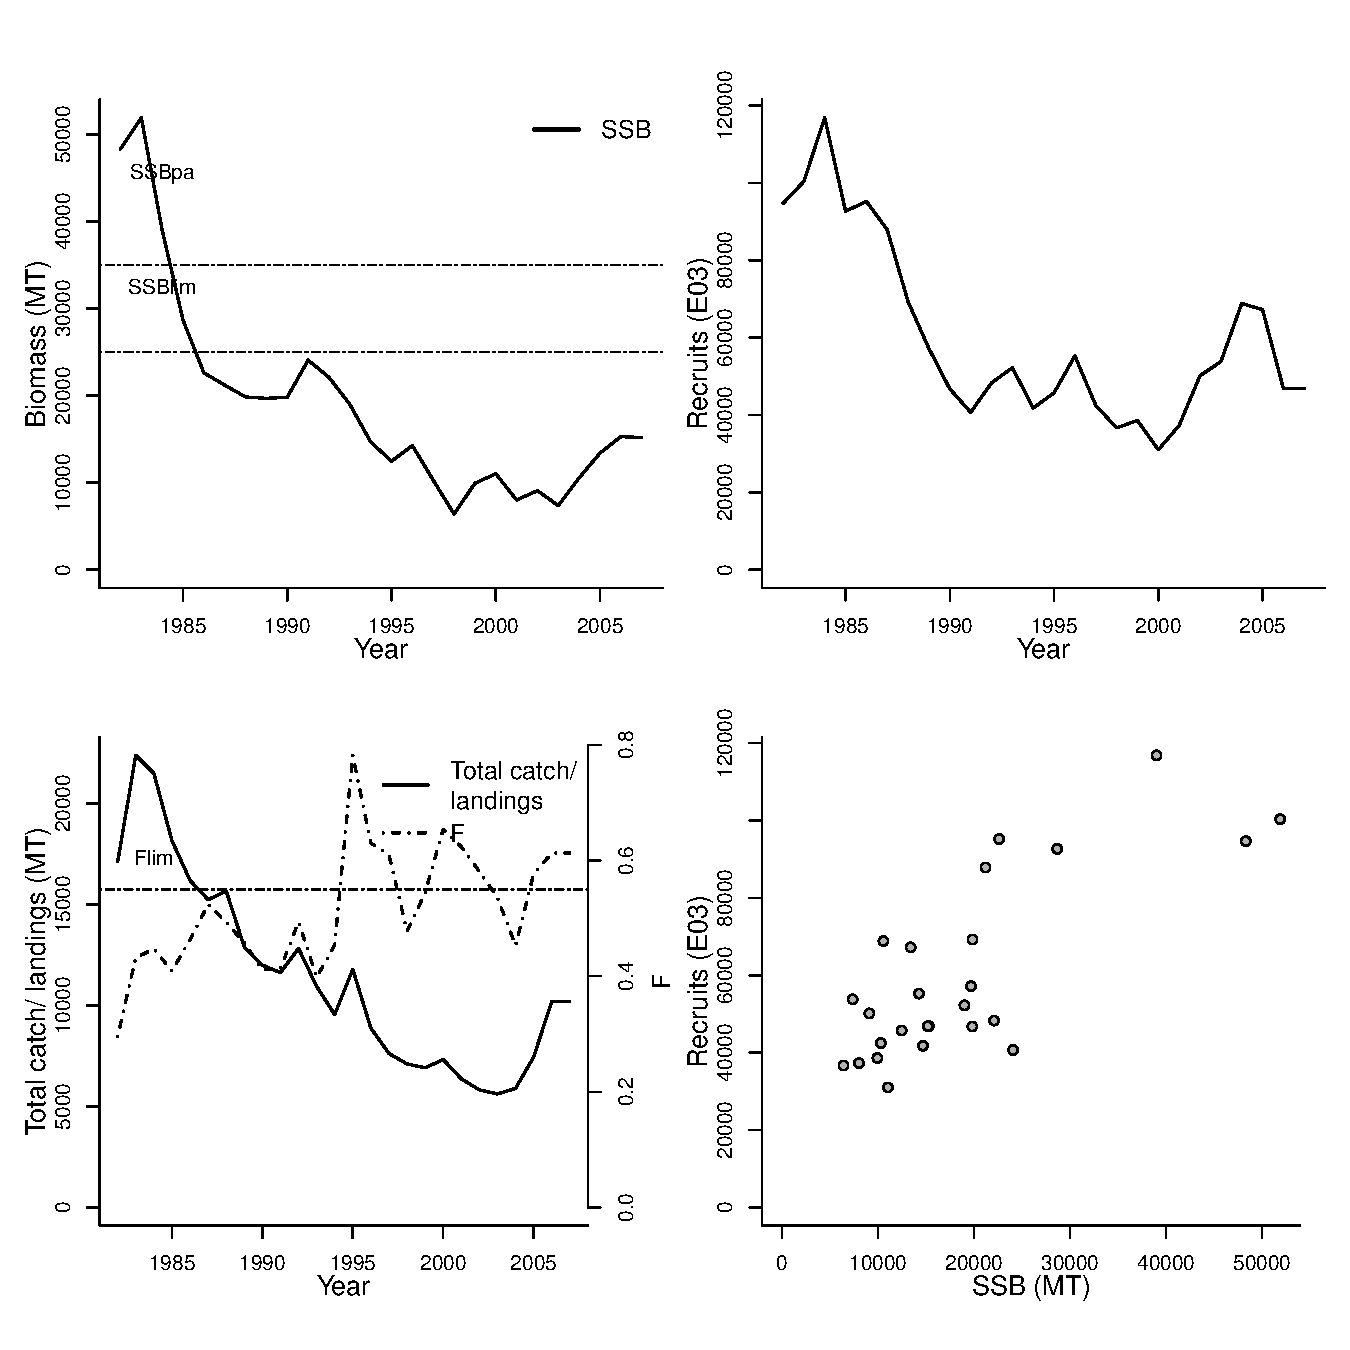
\includegraphics[scale=0.65]{../tex/figures/plot-WGHMM-HAKESOTH-1982-2007-JENNINGS.pdf}
\end{center}

\newpage
\section{Perciformes}\index{Perciformes}

\subsection{Gempylidae}\index{Gempylidae}\index{Perciformes!Gempylidae}

\subsubsection{Rexea solandri - common gemfish}\index{common gemfish}\index{Rexea solandri}\index{Gempylidae!Rexea solandri}
ID: CSIRO-GEMFISHSESSF-1966-2007-FULTON

common gemfish Southeast Australia 

stock assessment conducted: Stock Synthesis v2.0 model 
\begin{center}
\vspace{-0.2cm}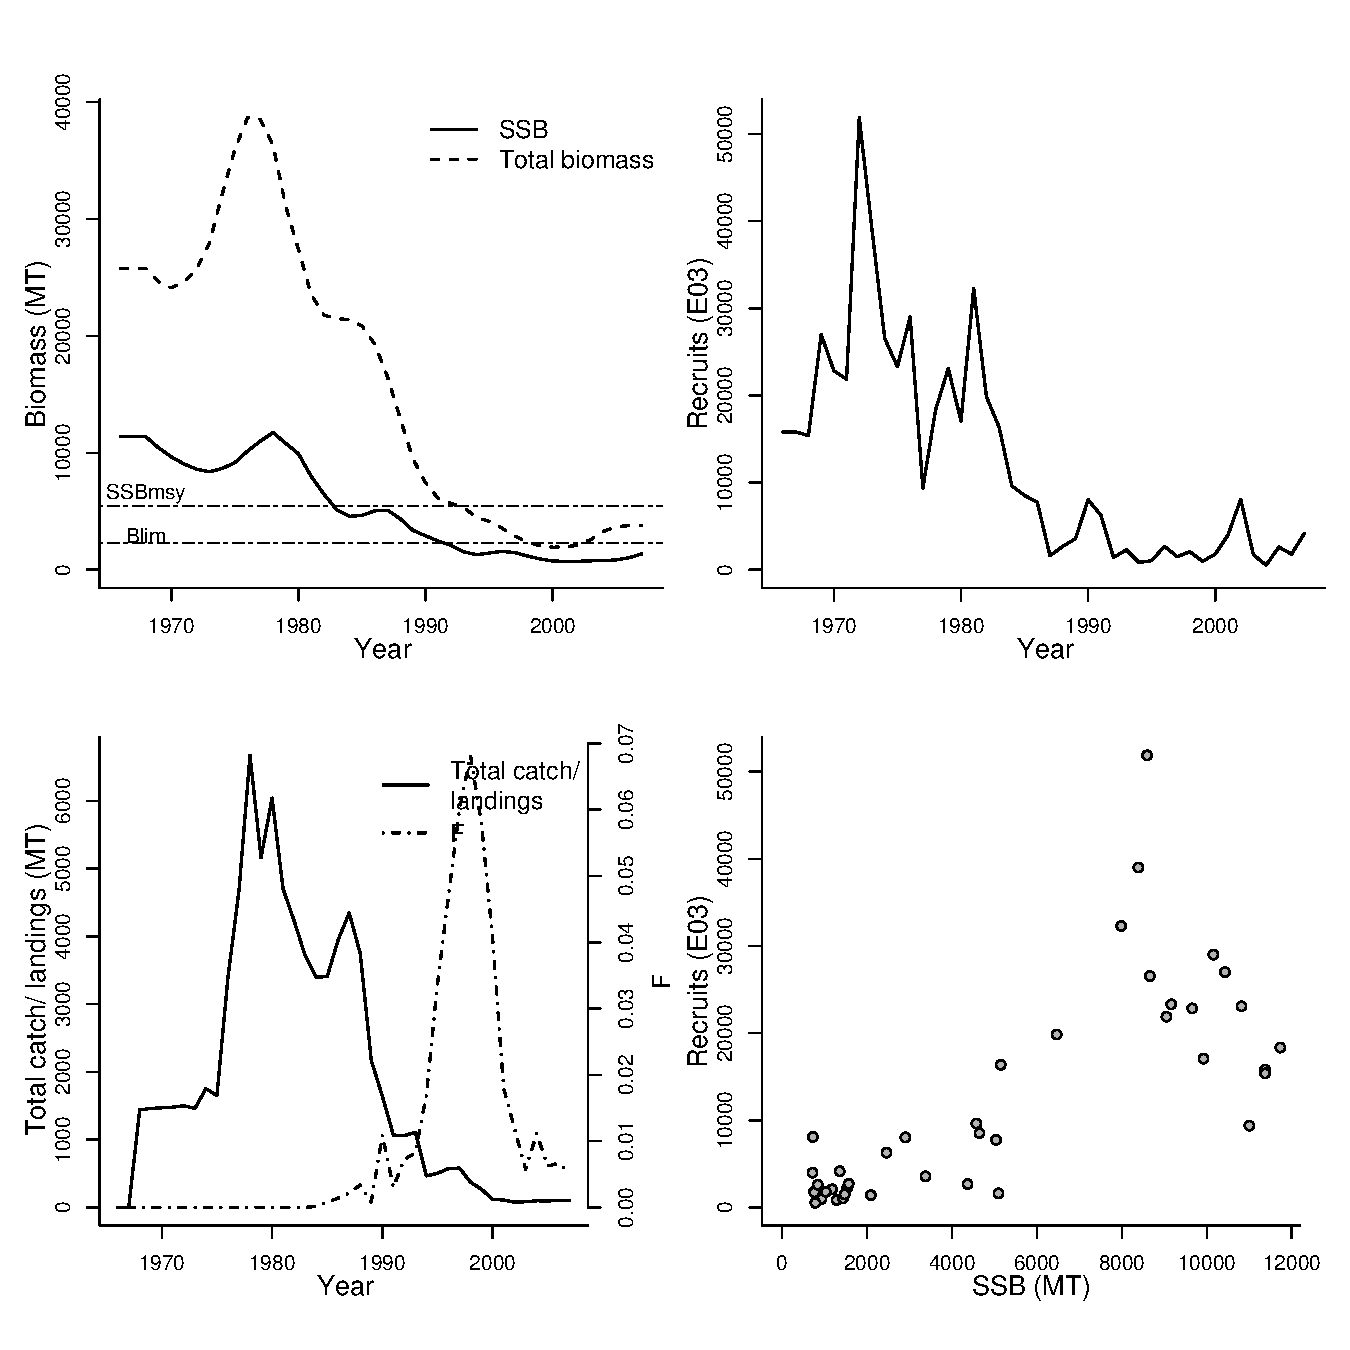
\includegraphics[scale=0.65]{../tex/figures/plot-CSIRO-GEMFISHSESSF-1966-2007-FULTON.pdf}
\end{center}

\newpage
\subsection{Labridae}\index{Labridae}\index{Perciformes!Labridae}

\subsubsection{Tautoga onitis - Tautog}\index{Tautog}\index{Tautoga onitis}\index{Labridae!Tautoga onitis}
ID: RIDEM-TAUTOGRI-1959-2007-COLLIE

Tautog Rhode Island 

stock assessment conducted: Age-aggregated surplus production model 
\begin{center}
\vspace{-0.2cm}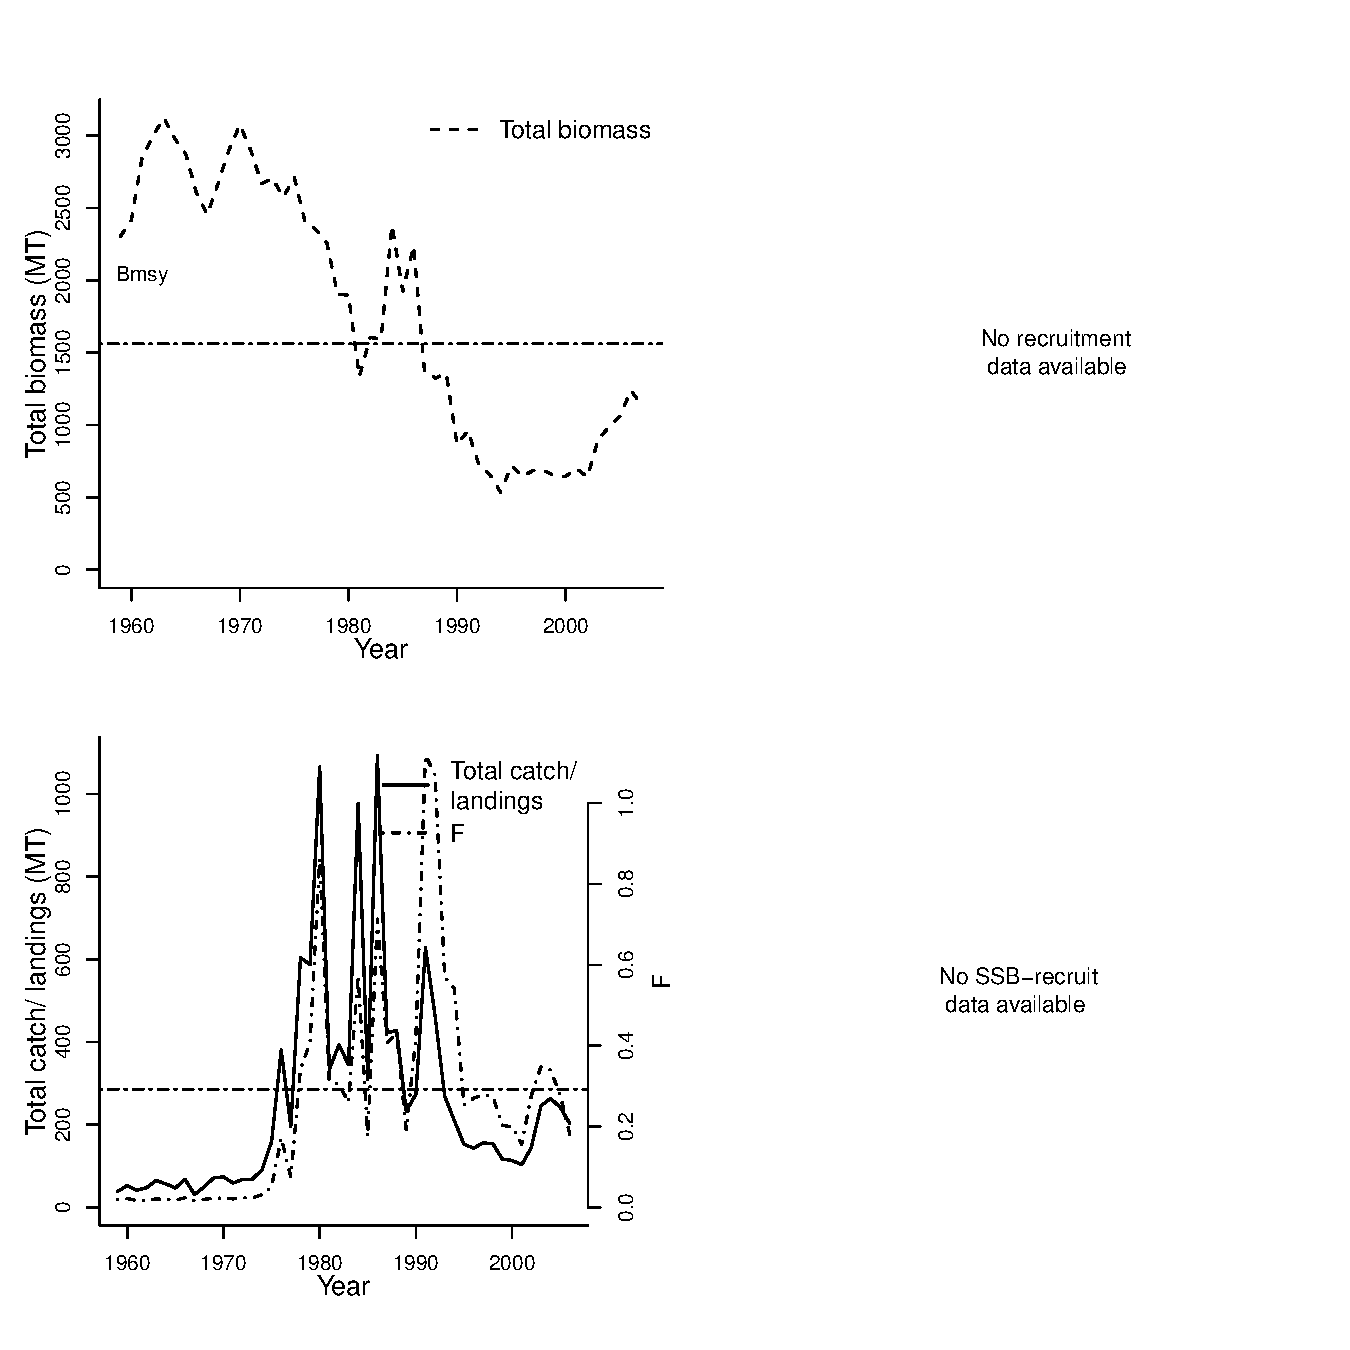
\includegraphics[scale=0.65]{../tex/figures/plot-RIDEM-TAUTOGRI-1959-2007-COLLIE.pdf}
\end{center}

\newpage
\subsection{Scombridae}\index{Scombridae}\index{Perciformes!Scombridae}

\subsubsection{Scomber scombrus - Mackerel}\index{Mackerel}\index{Scomber scombrus}\index{Scombridae!Scomber scombrus}
ID: WGMHSA-MACKNEICES-1972-2007-JENNINGS

Mackerel ICES Northeast Atlantic 

stock assessment conducted: Integrated Catch-at-age Analysis 
\begin{center}
\vspace{-0.2cm}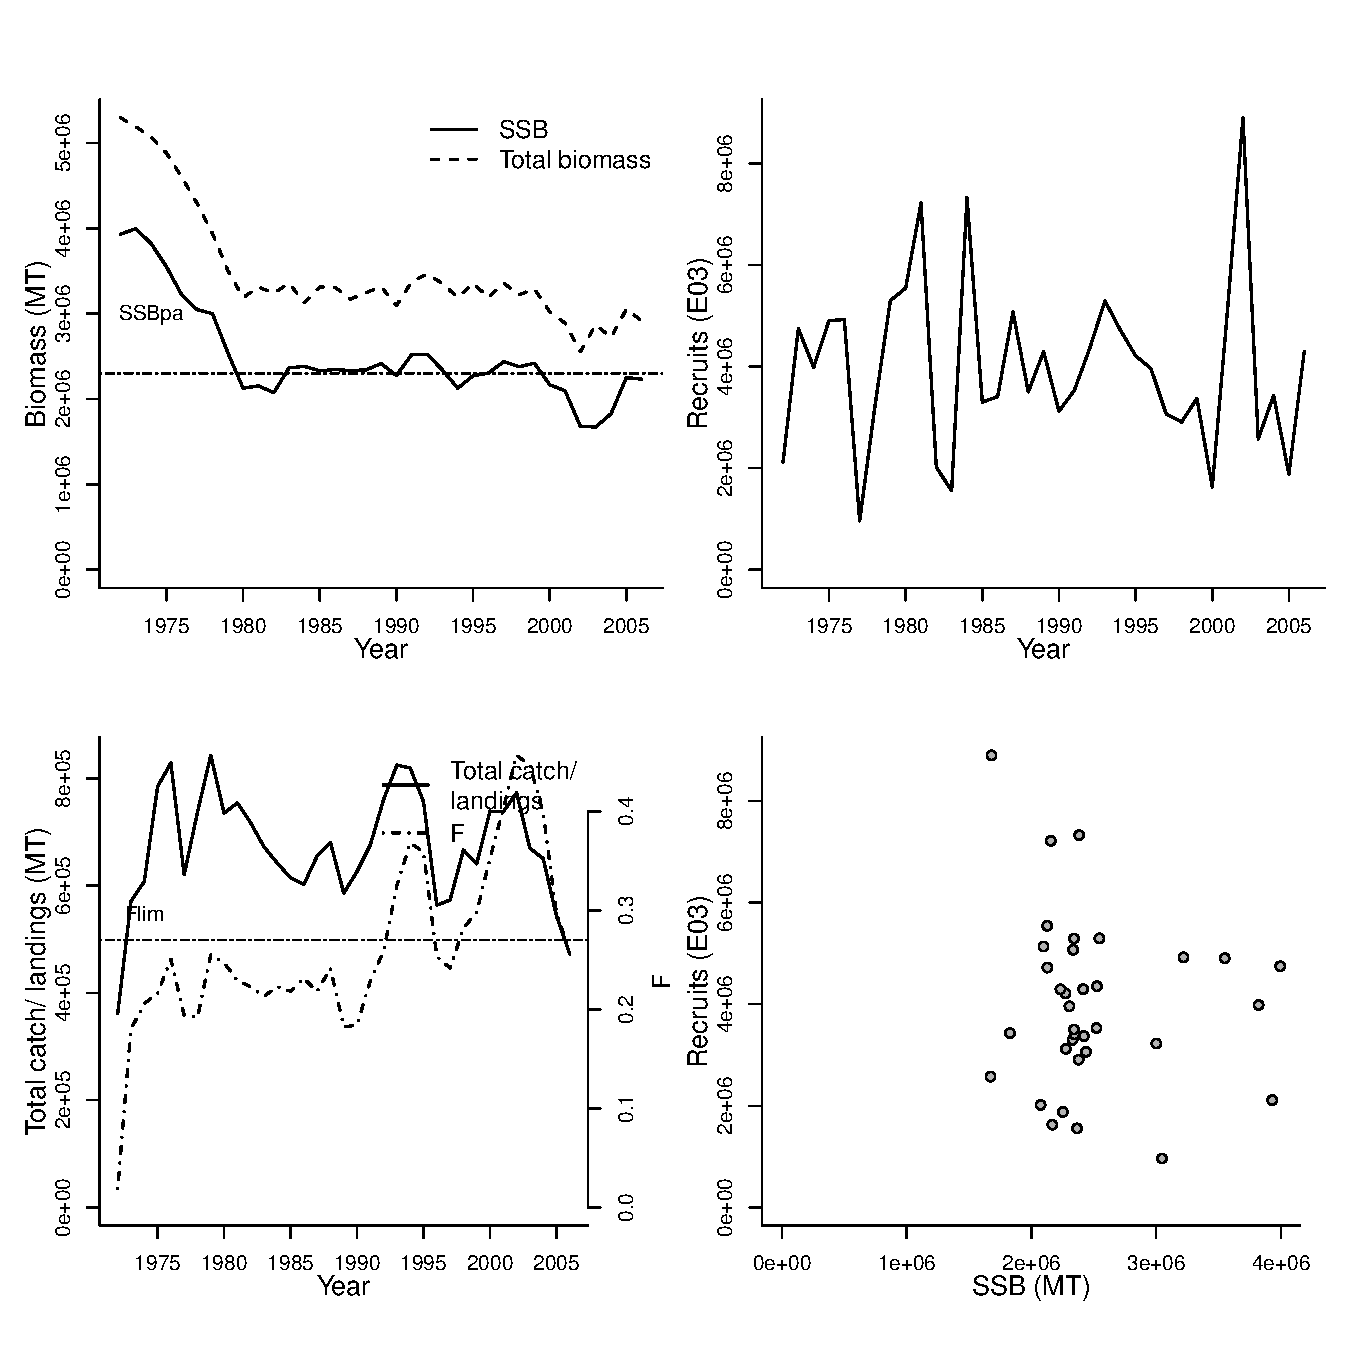
\includegraphics[scale=0.65]{../tex/figures/plot-WGMHSA-MACKNEICES-1972-2007-JENNINGS.pdf}
\end{center}

\newpage
\section{Pleuronectiformes}\index{Pleuronectiformes}

\subsection{Pleuronectidae}\index{Pleuronectidae}\index{Pleuronectiformes!Pleuronectidae}

\subsubsection{Hippoglossus stenolepis - Pacific halibut}\index{Pacific halibut}\index{Hippoglossus stenolepis}\index{Pleuronectidae!Hippoglossus stenolepis}
ID: IPHC-PHALNPAC-1988-2009-Parma

Pacific halibut North Pacific 

stock assessment conducted: an AD-Model builder statistical Catch at Age Model 
\begin{center}
\vspace{-0.2cm}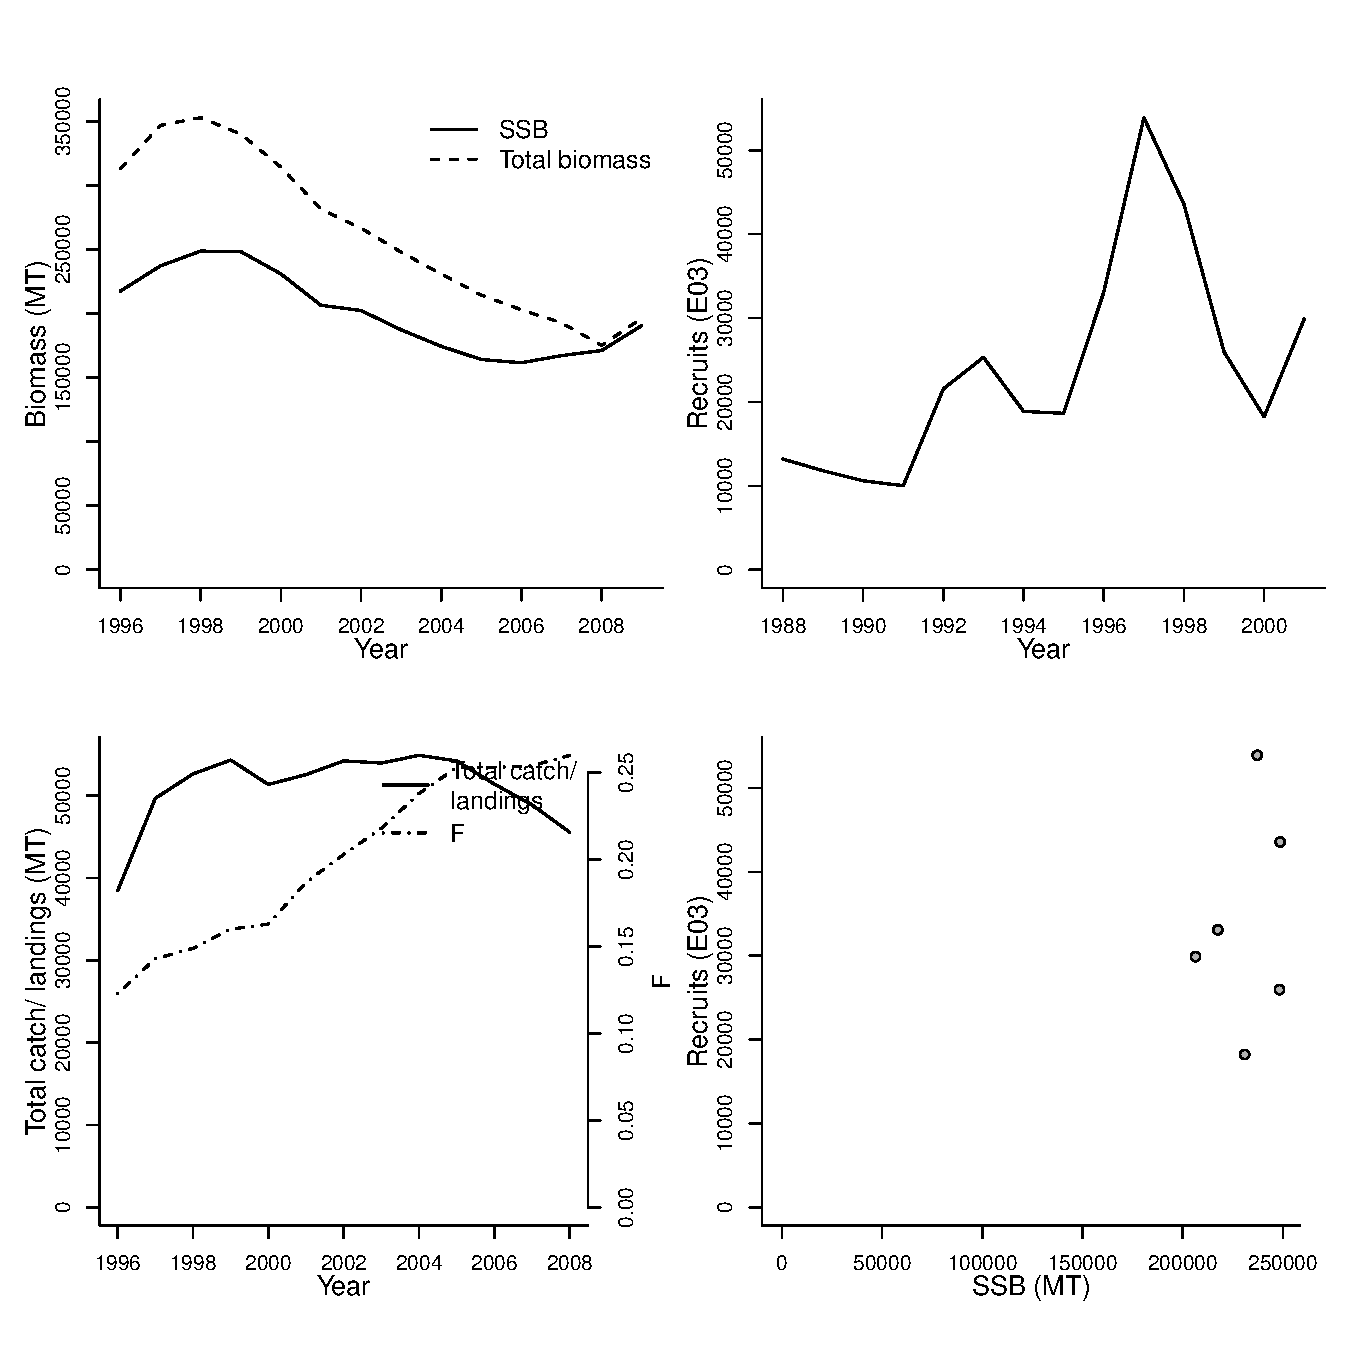
\includegraphics[scale=0.65]{../tex/figures/plot-IPHC-PHALNPAC-1988-2009-Parma.pdf}
\end{center}

\newpage
\subsubsection{Lepidopsetta bilineata - Rock sole}\index{Rock sole}\index{Lepidopsetta bilineata}\index{Pleuronectidae!Lepidopsetta bilineata}
ID: DFO-PAC-RSOLEHSTR-1945-2001-COLLIE

Rock sole Hecate Strait 

stock assessment conducted: State-space catch at age time series analysis 
\begin{center}
\vspace{-0.2cm}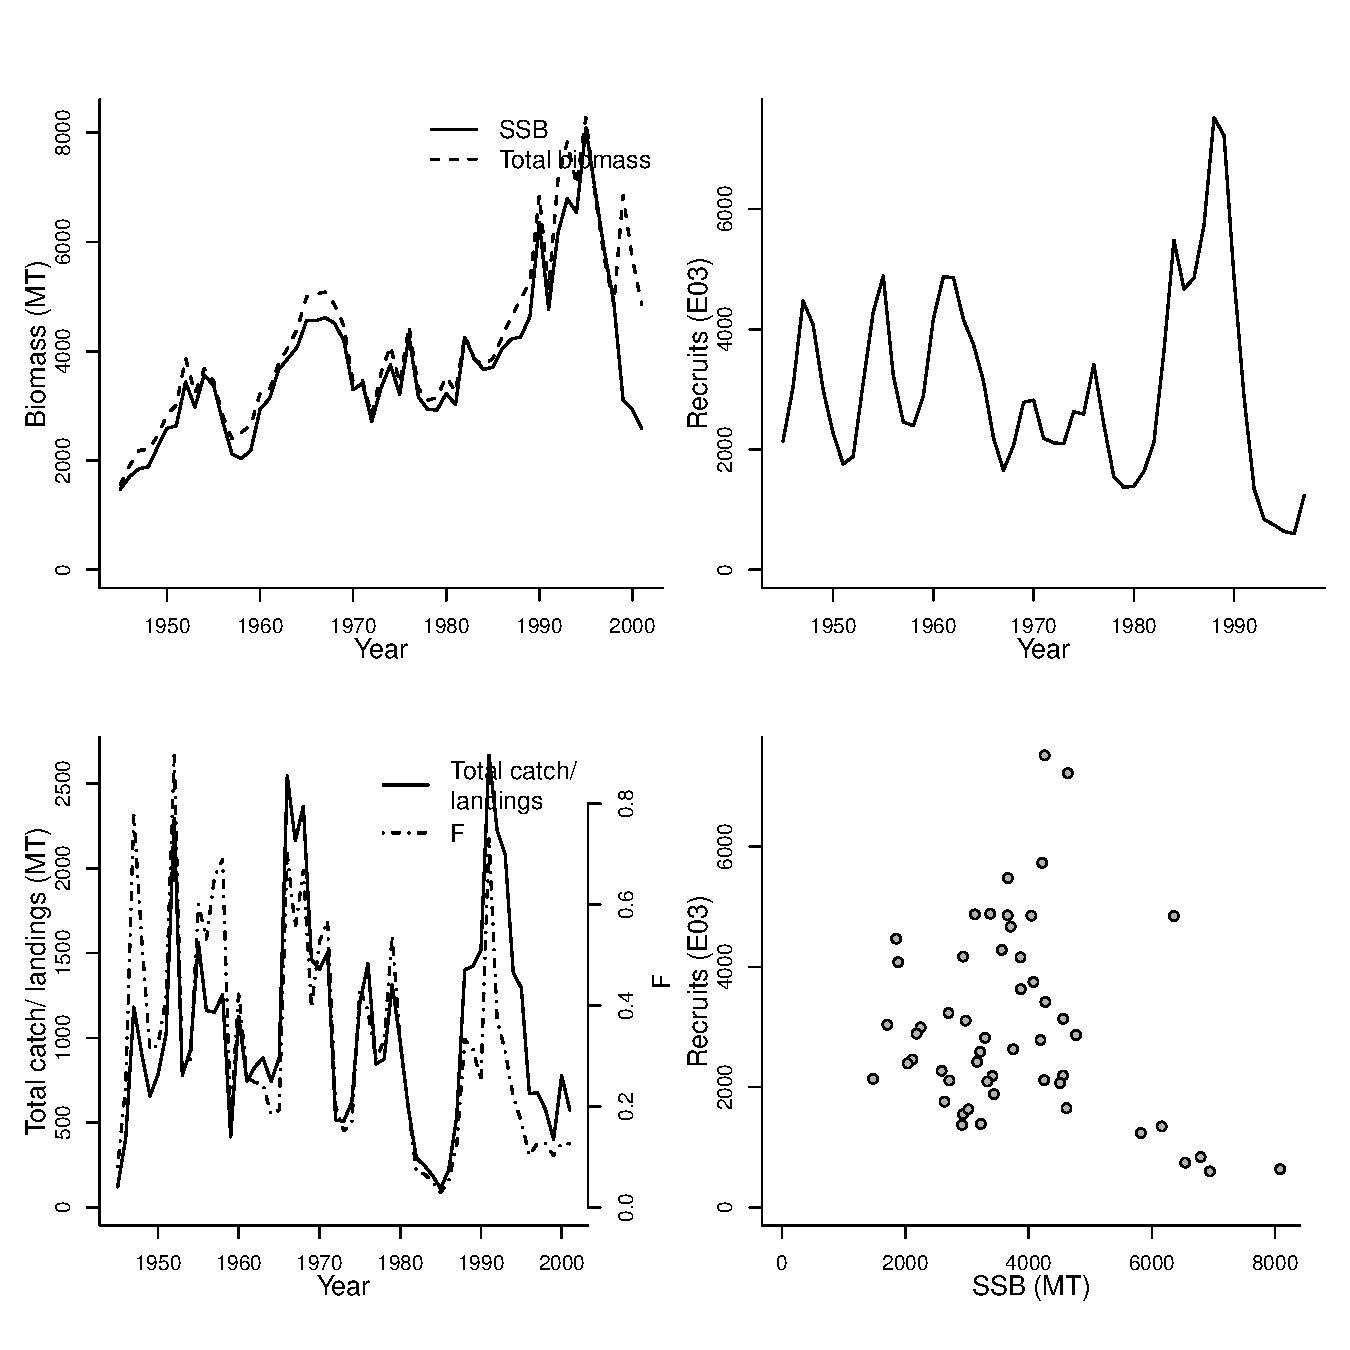
\includegraphics[scale=0.65]{../tex/figures/plot-DFO-PAC-RSOLEHSTR-1945-2001-COLLIE.pdf}
\end{center}

\newpage
\subsubsection{Parophrys vetulus - English sole}\index{English sole}\index{Parophrys vetulus}\index{Pleuronectidae!Parophrys vetulus}
ID: DFO-PAC-ESOLEHS-1944-2001-COLLIE

English sole Hecate Strait 

stock assessment conducted: State-space catch at age time series analysis 
\begin{center}
\vspace{-0.2cm}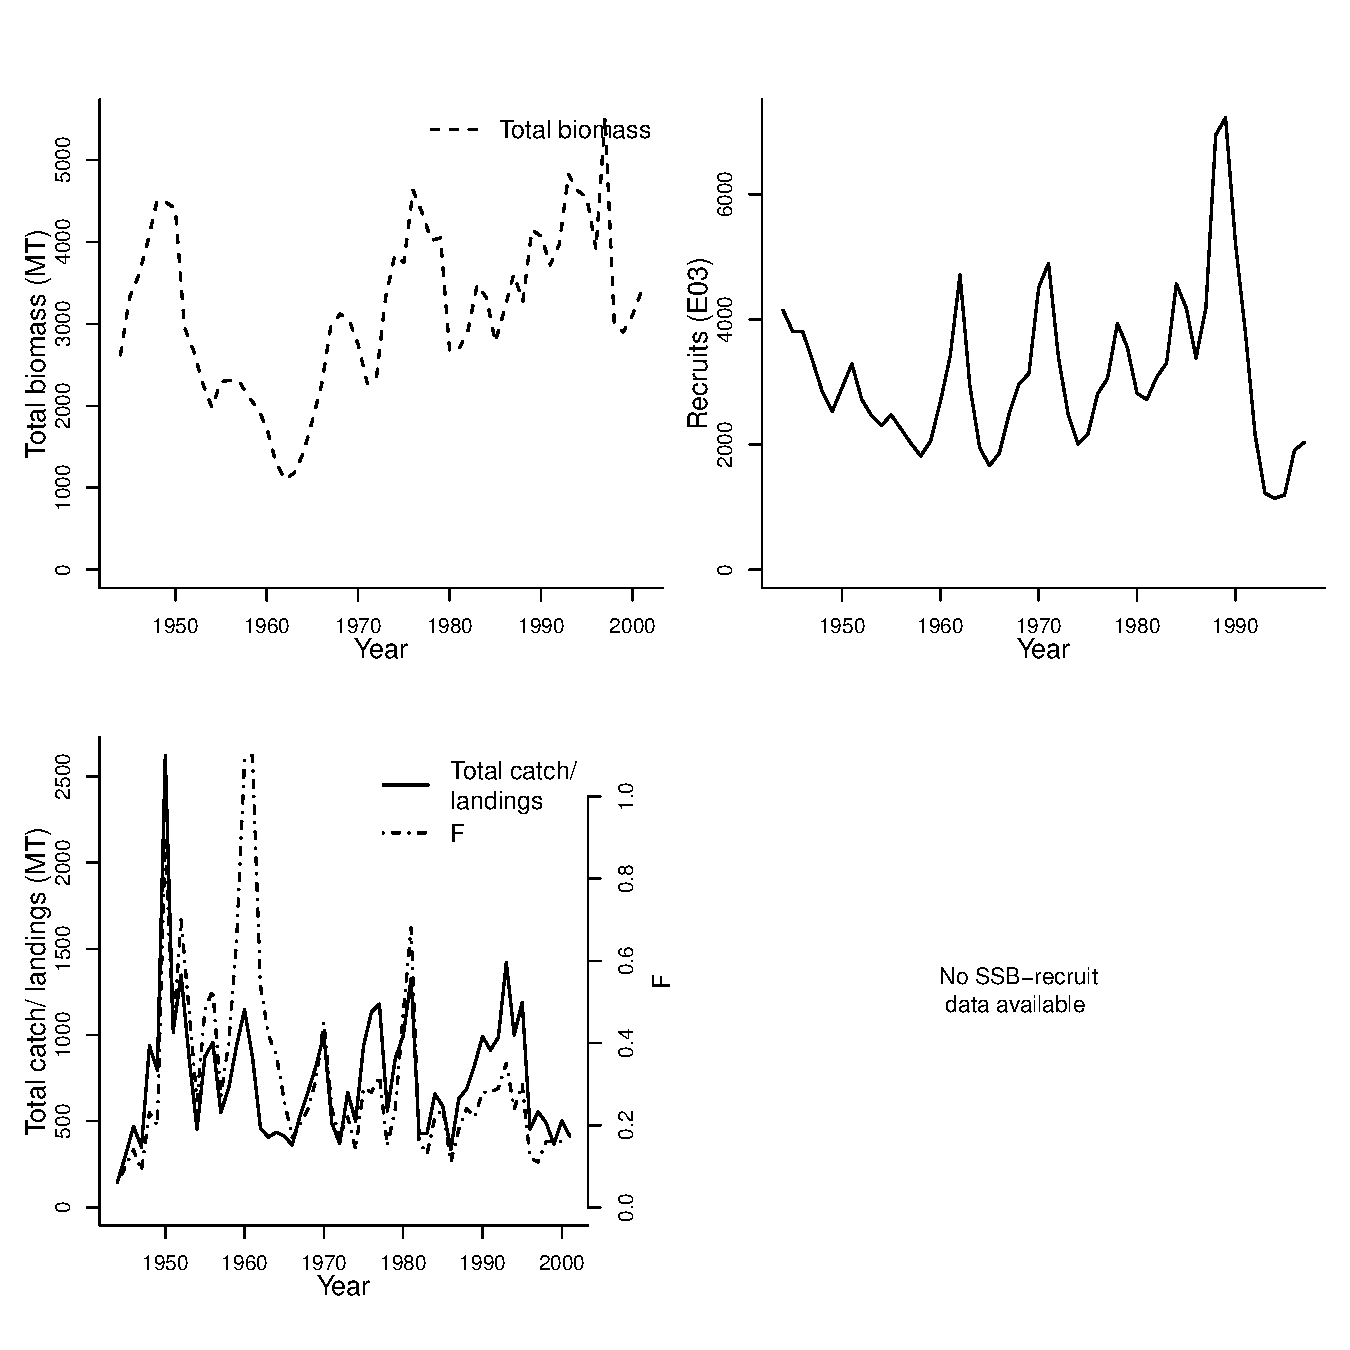
\includegraphics[scale=0.65]{../tex/figures/plot-DFO-PAC-ESOLEHS-1944-2001-COLLIE.pdf}
\end{center}

\newpage
\subsubsection{Pleuronectes platessa - European Plaice}\index{European Plaice}\index{Pleuronectes platessa}\index{Pleuronectidae!Pleuronectes platessa}
ID: WGSSDS-PLAICECHW-1975-2006-JENNINGS

European Plaice ICES VIIe 

stock assessment conducted: Extended Survivor Analysis 
\begin{center}
\vspace{-0.2cm}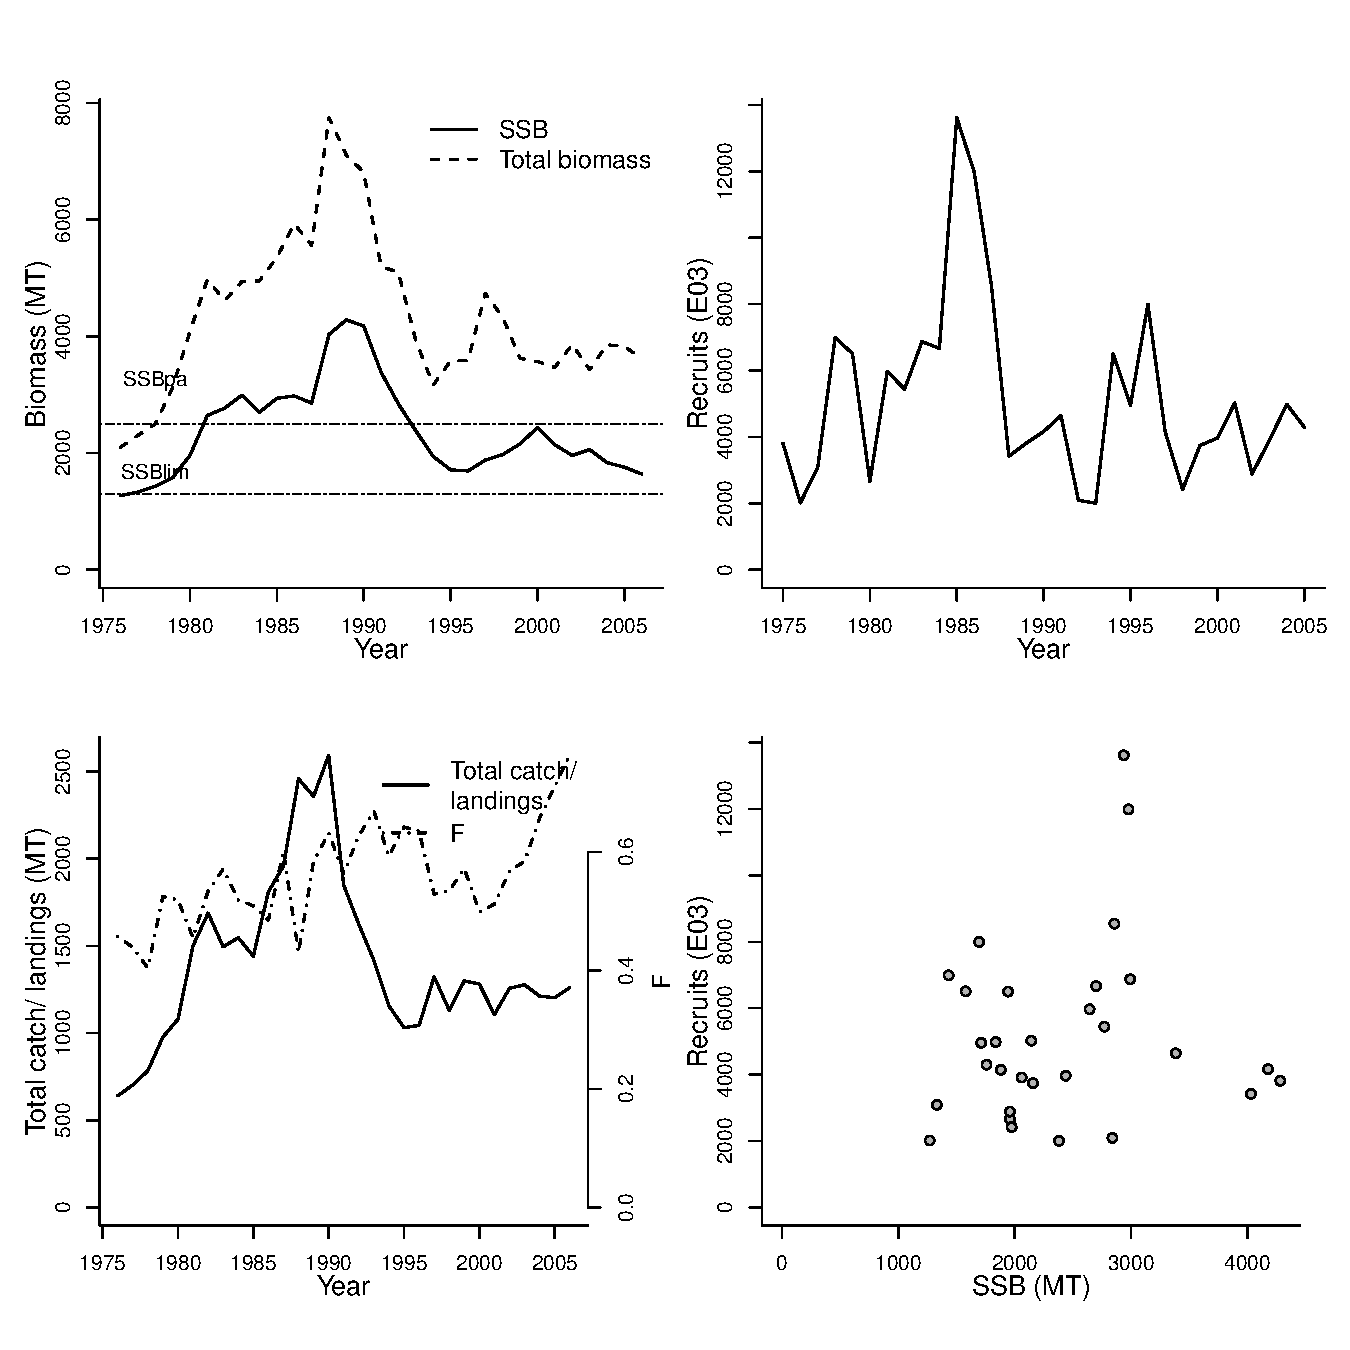
\includegraphics[scale=0.65]{../tex/figures/plot-WGSSDS-PLAICECHW-1975-2006-JENNINGS.pdf}
\end{center}

\newpage
\subsubsection{Pleuronectes platessa - European Plaice}\index{European Plaice}\index{Pleuronectes platessa}\index{Pleuronectidae!Pleuronectes platessa}
ID: WGSSDS-PLAICCELT-1976-2006-JENNINGS

European Plaice ICES VIIf-g 

stock assessment conducted: Extended Survivor Analysis 
\begin{center}
\vspace{-0.2cm}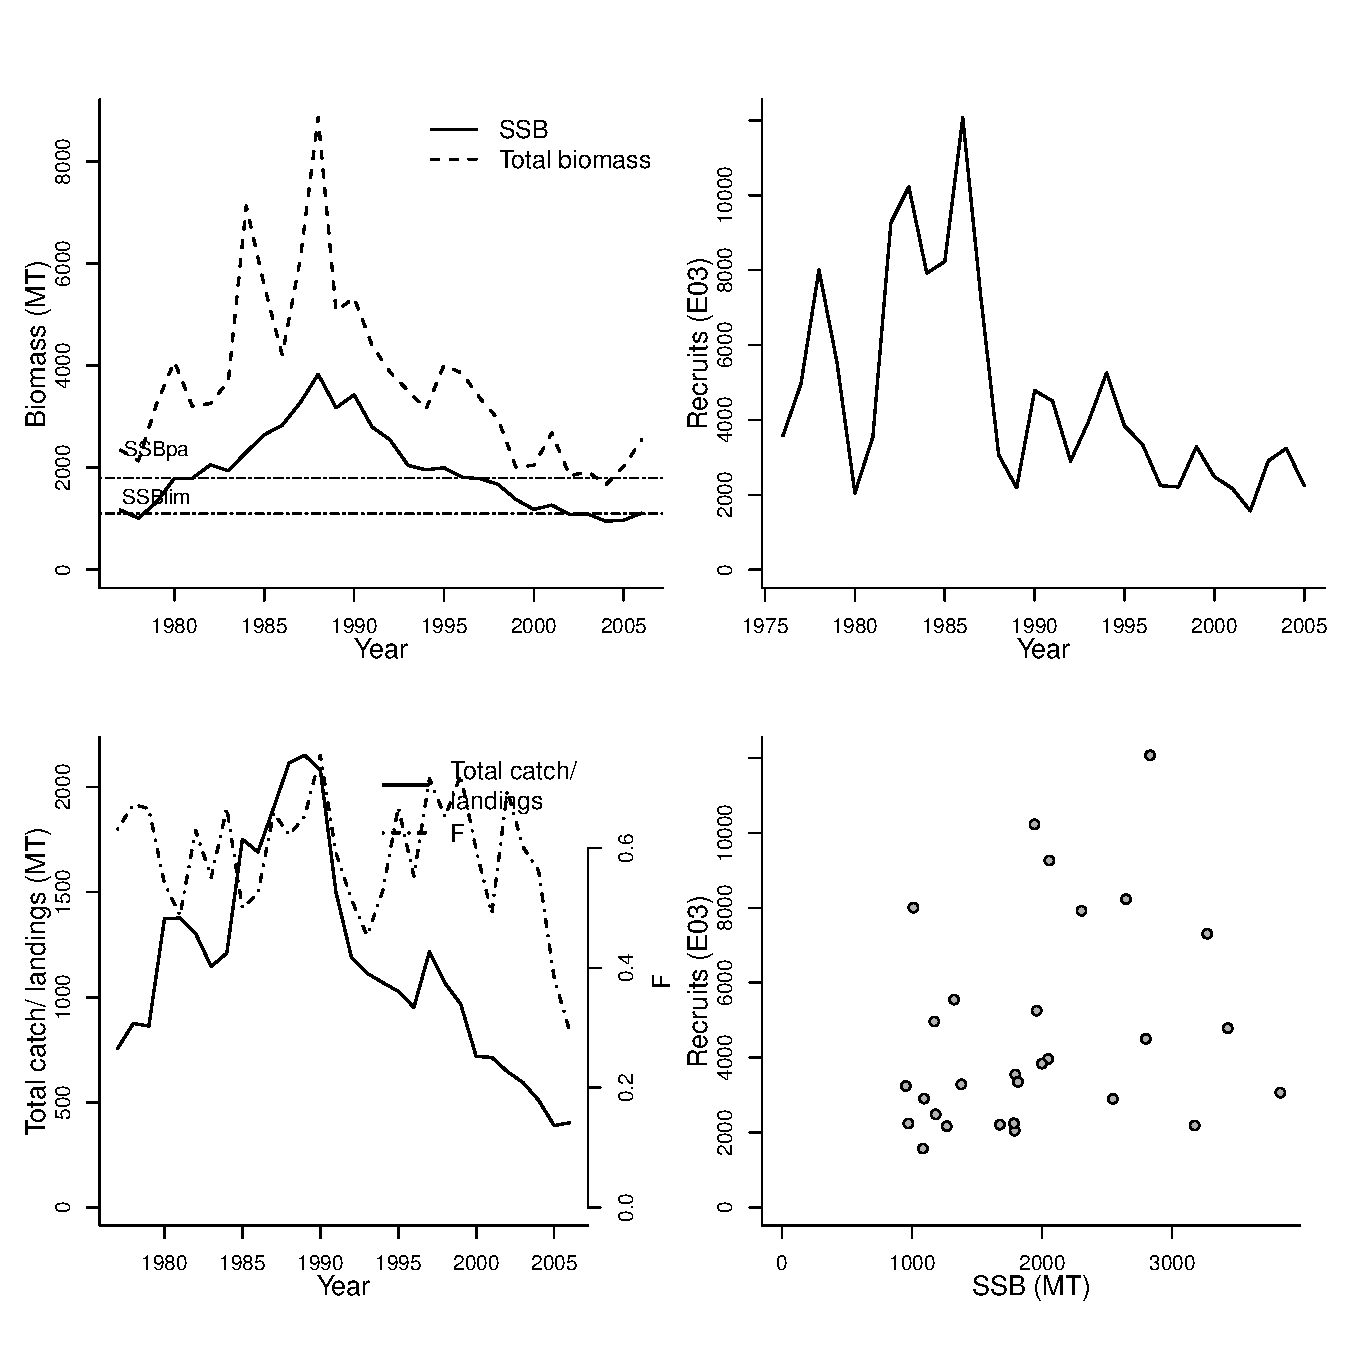
\includegraphics[scale=0.65]{../tex/figures/plot-WGSSDS-PLAICCELT-1976-2006-JENNINGS.pdf}
\end{center}

\newpage
\subsubsection{Pseudopleuronectes americanus - Winter flounder}\index{Winter flounder}\index{Pseudopleuronectes americanus}\index{Pleuronectidae!Pseudopleuronectes americanus}
ID: RIDEM-WINFLOUNDRI-1959-2007-COLLIE

Winter flounder Rhode Island 

stock assessment conducted: Age-aggregated surplus production model 
\begin{center}
\vspace{-0.2cm}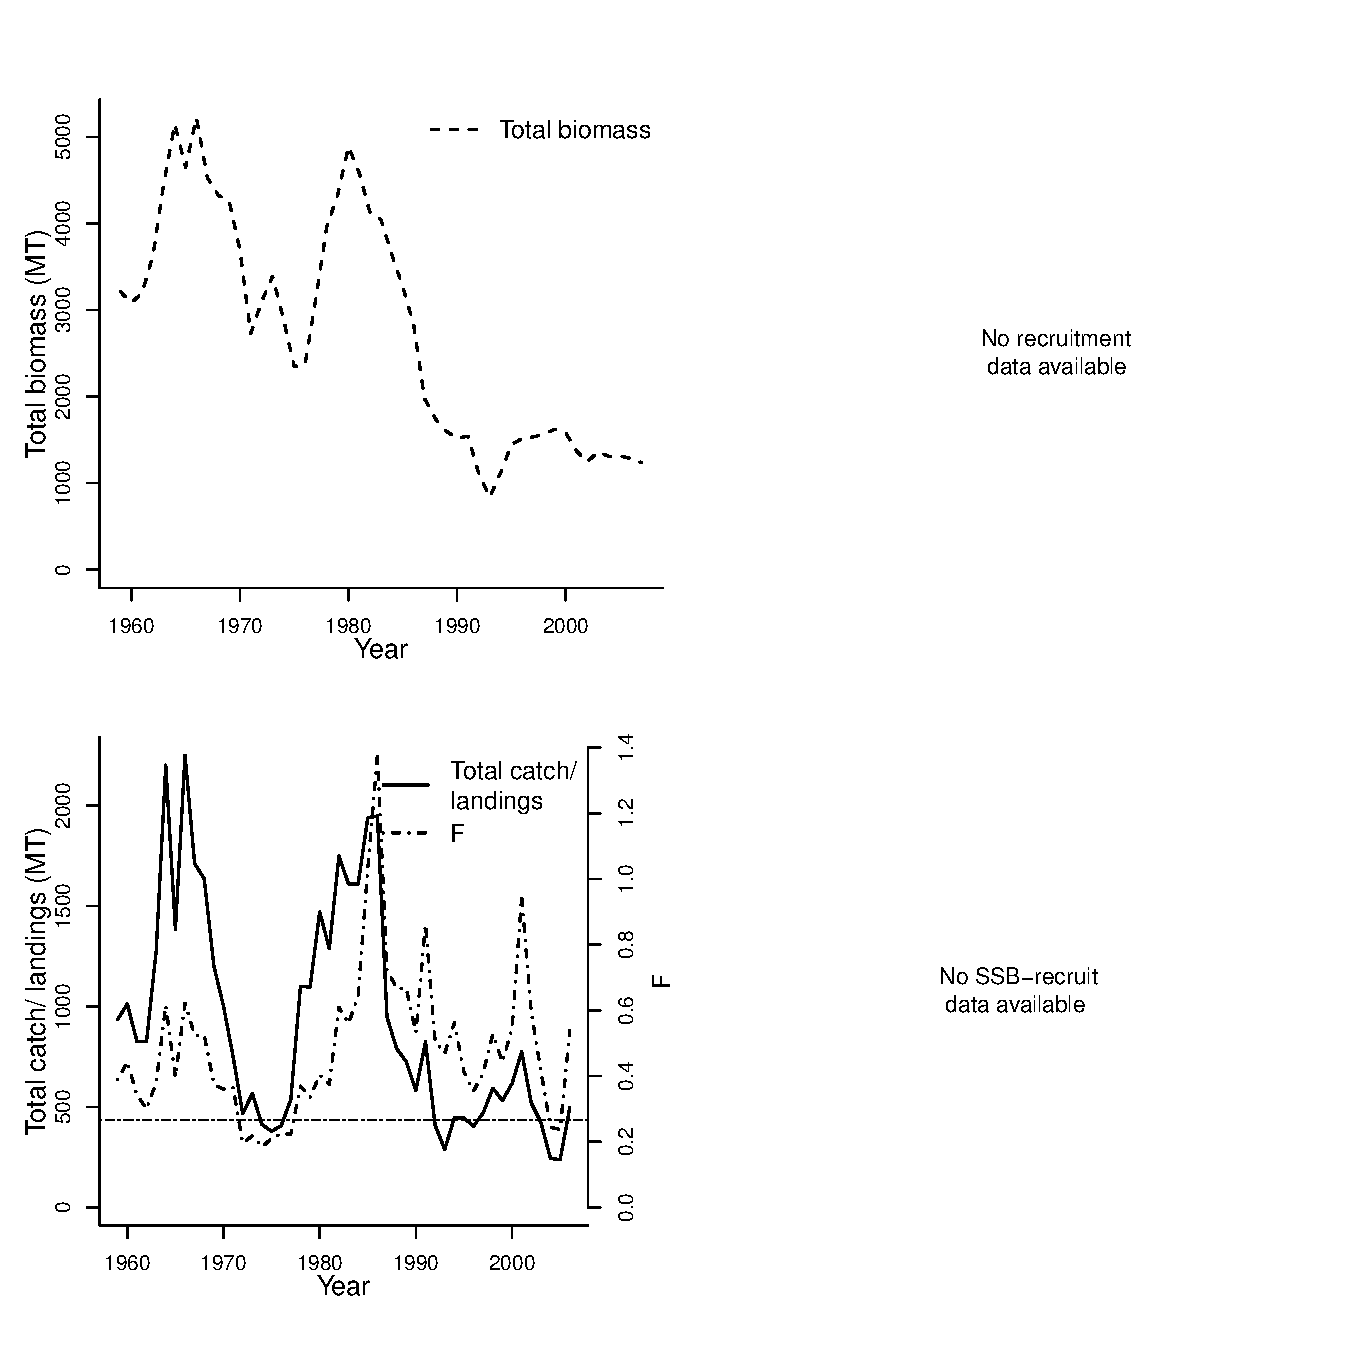
\includegraphics[scale=0.65]{../tex/figures/plot-RIDEM-WINFLOUNDRI-1959-2007-COLLIE.pdf}
\end{center}

\newpage
\subsubsection{Reinhardtius hippoglossoides - Greenland halibut}\index{Greenland halibut}\index{Reinhardtius hippoglossoides}\index{Pleuronectidae!Reinhardtius hippoglossoides}
ID: AFWG-GHALNEAR-1959-2007-JENNINGS

Greenland halibut Northeast Arctic 

stock assessment conducted: Extended Survivor Analysis 
\begin{center}
\vspace{-0.2cm}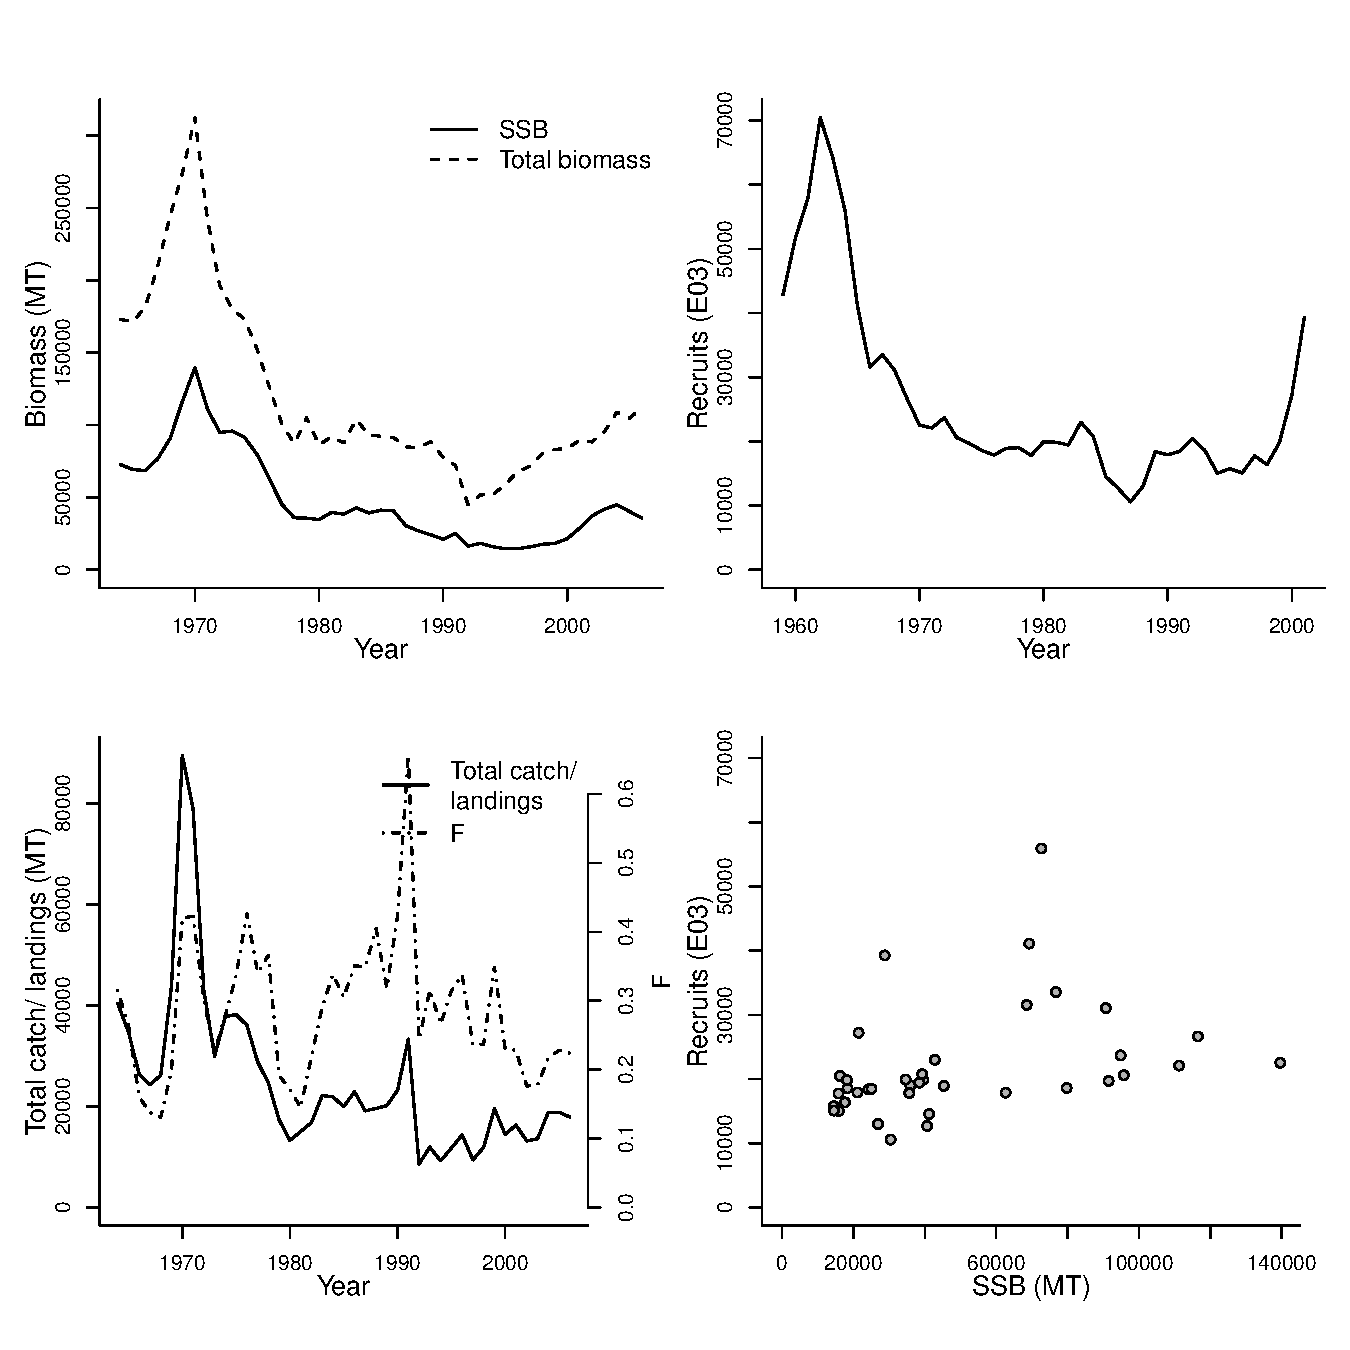
\includegraphics[scale=0.65]{../tex/figures/plot-AFWG-GHALNEAR-1959-2007-JENNINGS.pdf}
\end{center}

\newpage
\subsubsection{Reinhardtius stomias - Arrowtooth flounder}\index{Arrowtooth flounder}\index{Reinhardtius stomias}\index{Pleuronectidae!Reinhardtius stomias}
ID: NWFSC-ARFLOUNDPCOAST-1916-2007-BRANCH

Arrowtooth flounder Pacific Coast 

stock assessment conducted: Stock Synthesis v2.0 model 
\begin{center}
\vspace{-0.2cm}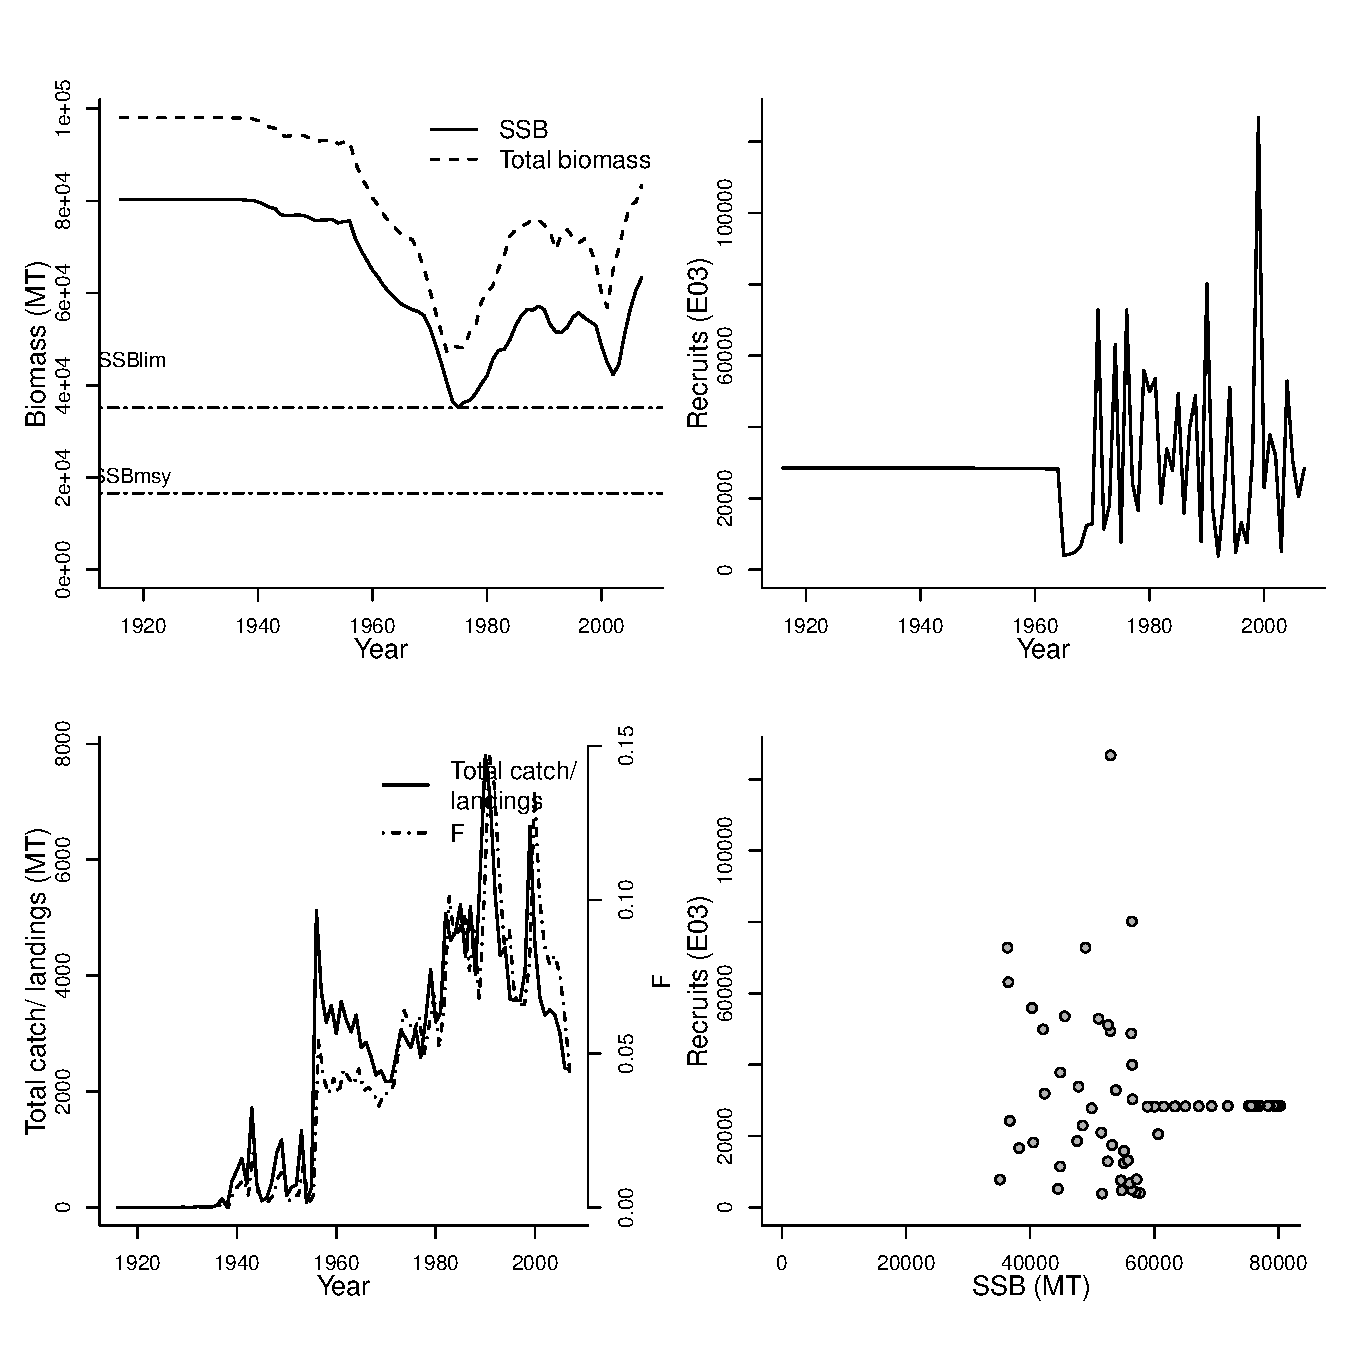
\includegraphics[scale=0.65]{../tex/figures/plot-NWFSC-ARFLOUNDPCOAST-1916-2007-BRANCH.pdf}
\end{center}

\newpage
\subsection{Scophthalmidae}\index{Scophthalmidae}\index{Pleuronectiformes!Scophthalmidae}

\subsubsection{Lepidorhombus boscii - Fourspotted megrim}\index{Fourspotted megrim}\index{Lepidorhombus boscii}\index{Scophthalmidae!Lepidorhombus boscii}
ID: WGHMM-FMEG8c9a-1986-2006-JENNINGS

Fourspotted megrim ICES VIIIc-IXa 

stock assessment conducted: Extended Survivor Analysis 
\begin{center}
\vspace{-0.2cm}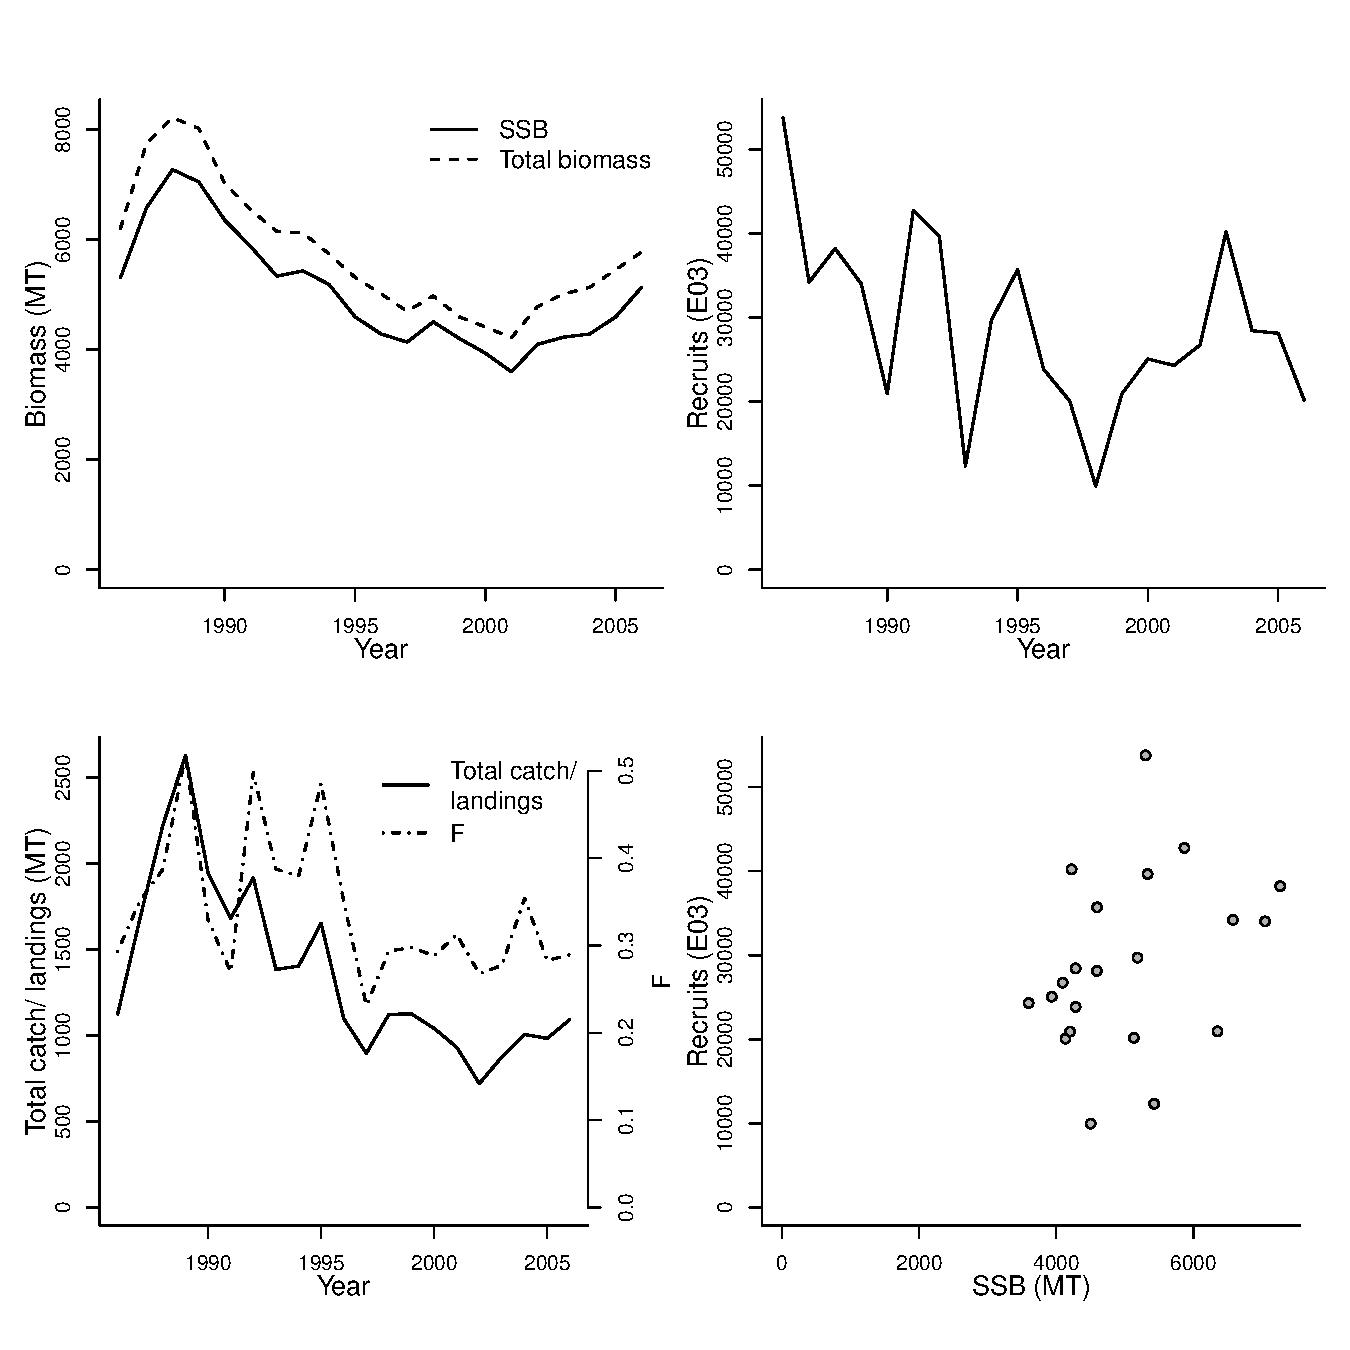
\includegraphics[scale=0.65]{../tex/figures/plot-WGHMM-FMEG8c9a-1986-2006-JENNINGS.pdf}
\end{center}

\newpage
\subsubsection{Lepidorhombus whiffiagonis - Megrim}\index{Megrim}\index{Lepidorhombus whiffiagonis}\index{Scophthalmidae!Lepidorhombus whiffiagonis}
ID: WGHMM-MEG8c9a-1985-2007-JENNINGS

Megrim ICES VIIIc-IXa 

stock assessment conducted: Extended Survivor Analysis 
\begin{center}
\vspace{-0.2cm}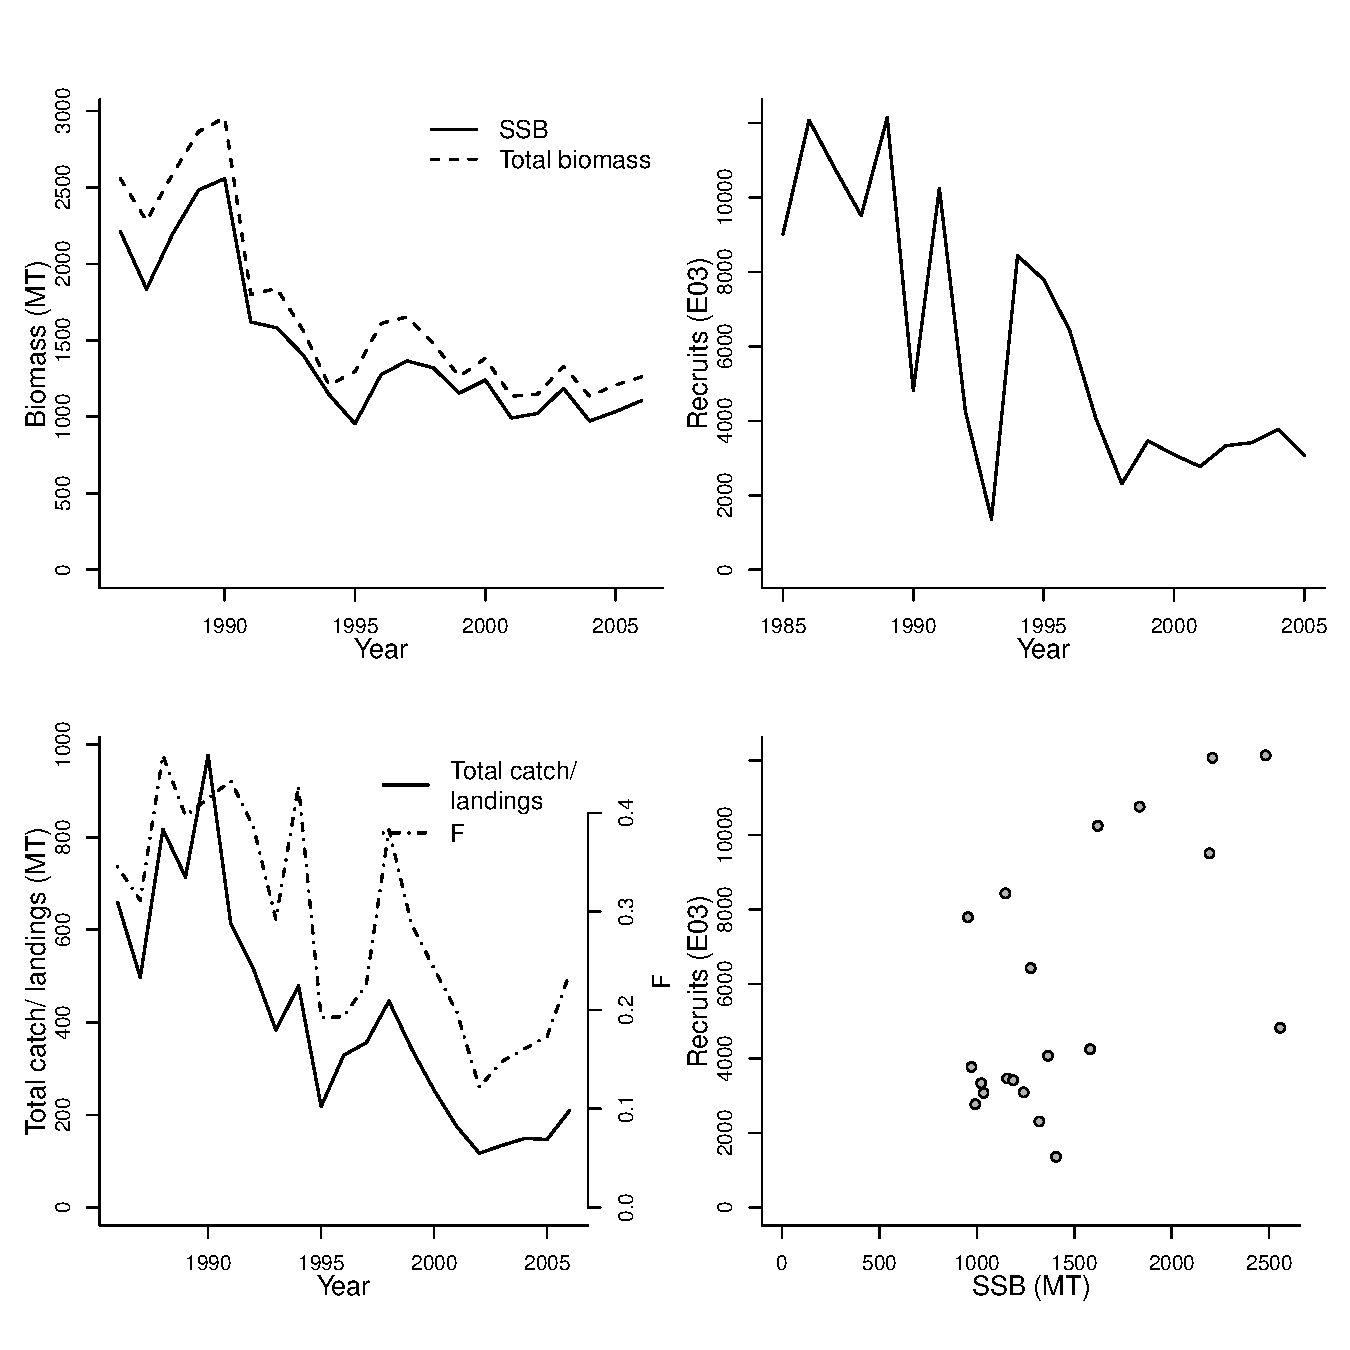
\includegraphics[scale=0.65]{../tex/figures/plot-WGHMM-MEG8c9a-1985-2007-JENNINGS.pdf}
\end{center}

\newpage
\subsection{Soleidae}\index{Soleidae}\index{Pleuronectiformes!Soleidae}

\subsubsection{Solea vulgaris - common European sole}\index{common European sole}\index{Solea vulgaris}\index{Soleidae!Solea vulgaris}
ID: WGHMM-SOLEVIII-1982-2006-JENNINGS

common European sole Bay of Biscay 

stock assessment conducted: Extended Survivor Analysis 
\begin{center}
\vspace{-0.2cm}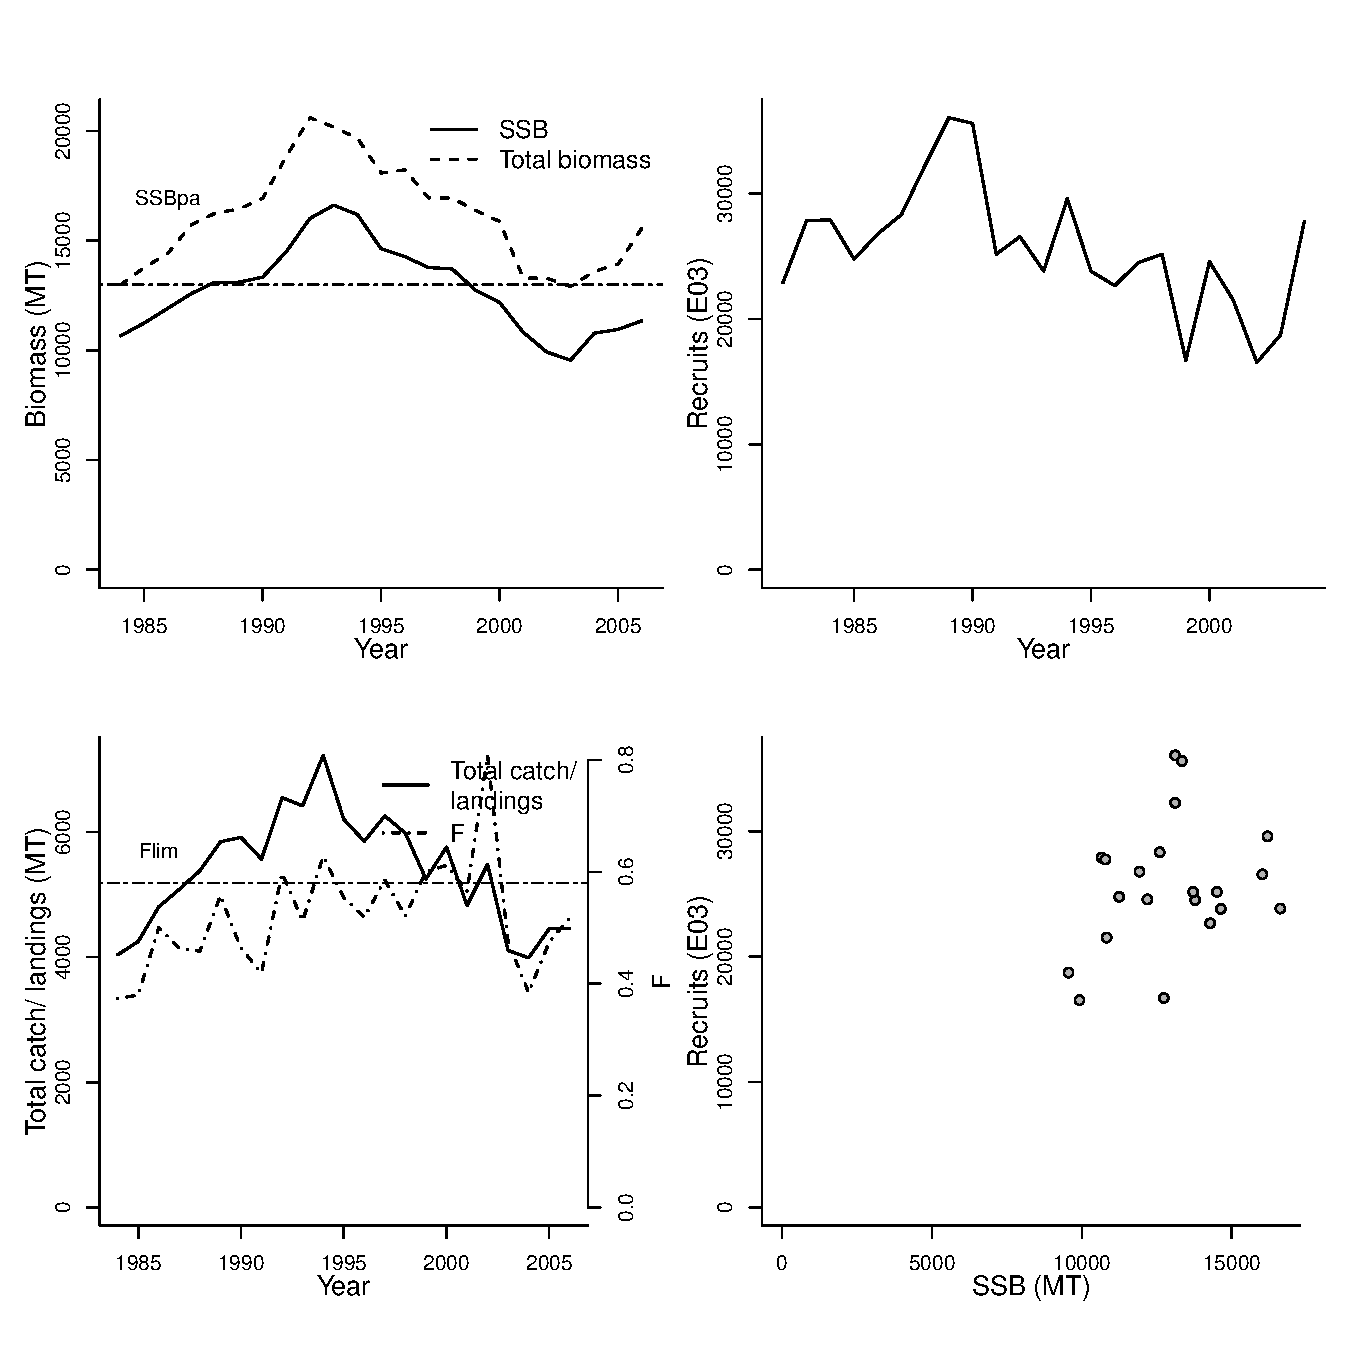
\includegraphics[scale=0.65]{../tex/figures/plot-WGHMM-SOLEVIII-1982-2006-JENNINGS.pdf}
\end{center}

\newpage
\subsubsection{Solea vulgaris - common European sole}\index{common European sole}\index{Solea vulgaris}\index{Soleidae!Solea vulgaris}
ID: WGSSDS-SOLECS-1970-2006-JENNINGS

common European sole Celtic Sea 

stock assessment conducted: Extended Survivor Analysis 
\begin{center}
\vspace{-0.2cm}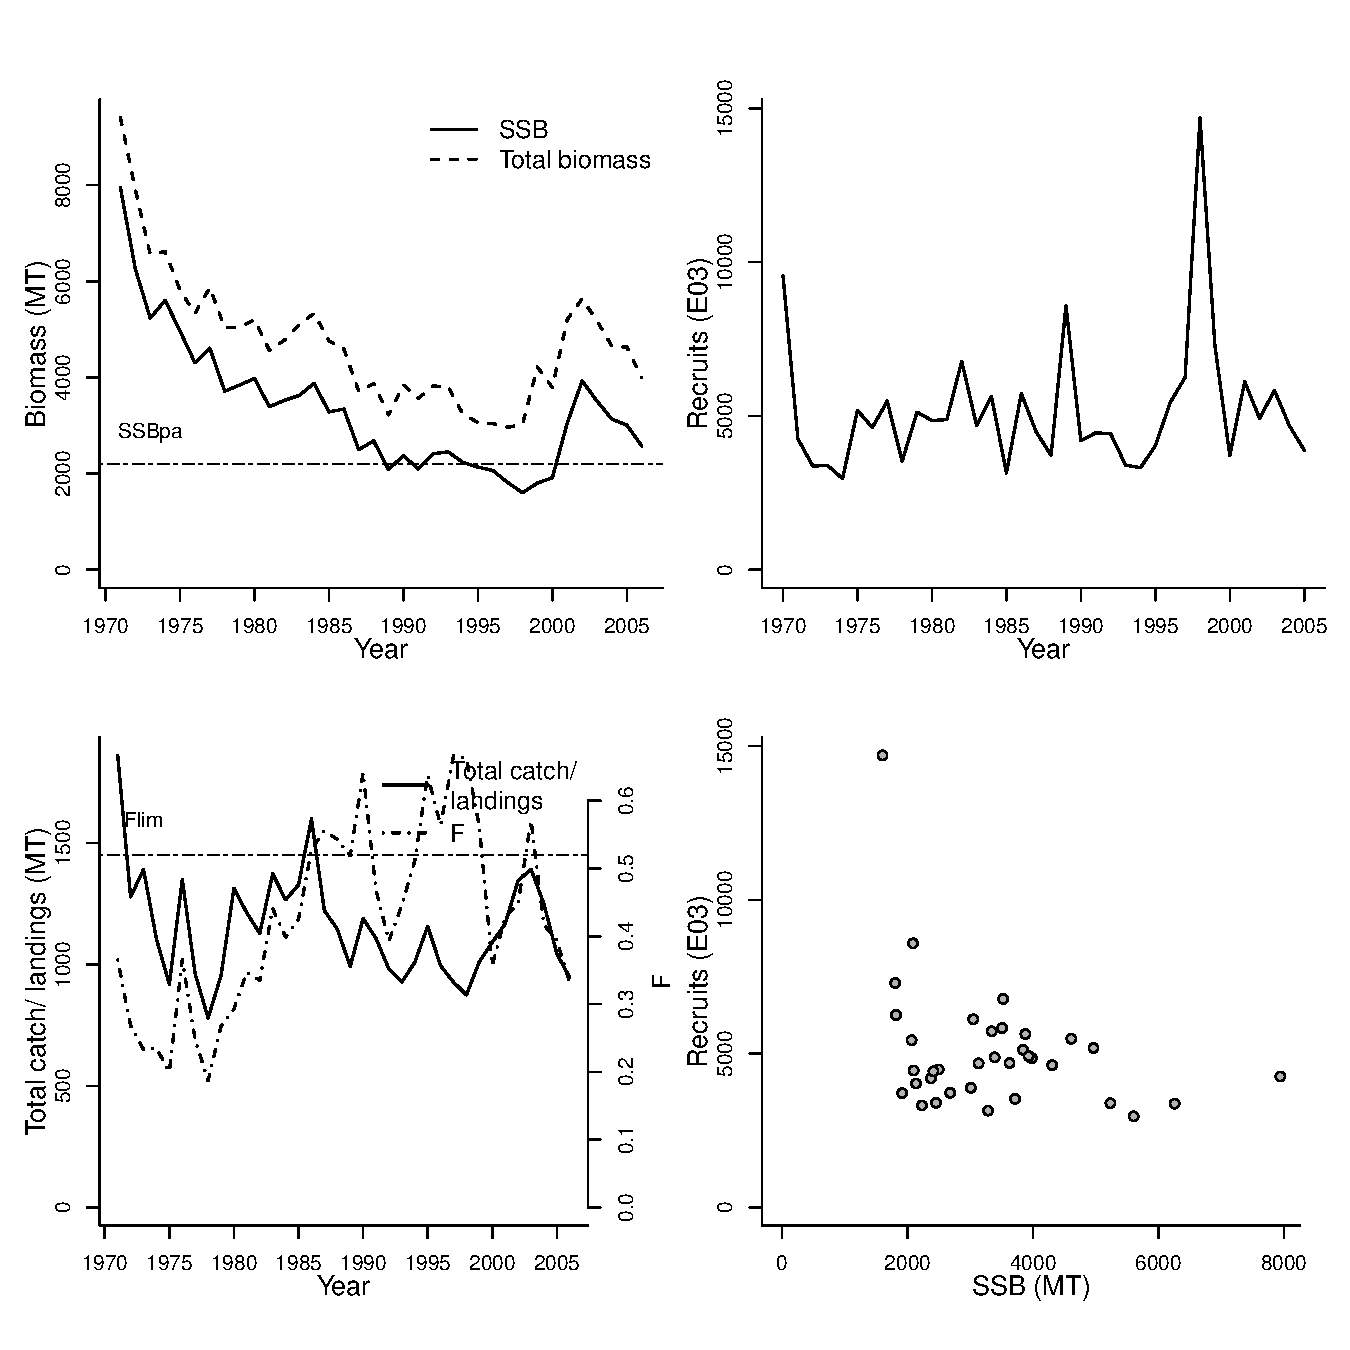
\includegraphics[scale=0.65]{../tex/figures/plot-WGSSDS-SOLECS-1970-2006-JENNINGS.pdf}
\end{center}

\newpage
\subsubsection{Solea vulgaris - common European sole}\index{common European sole}\index{Solea vulgaris}\index{Soleidae!Solea vulgaris}
ID: WGBFAS-SOLEIIIa-1982-2007-JENNINGS

common European sole ICES Kattegat and Skagerrak 

stock assessment conducted: Extended Survivor Analysis 
\begin{center}
\vspace{-0.2cm}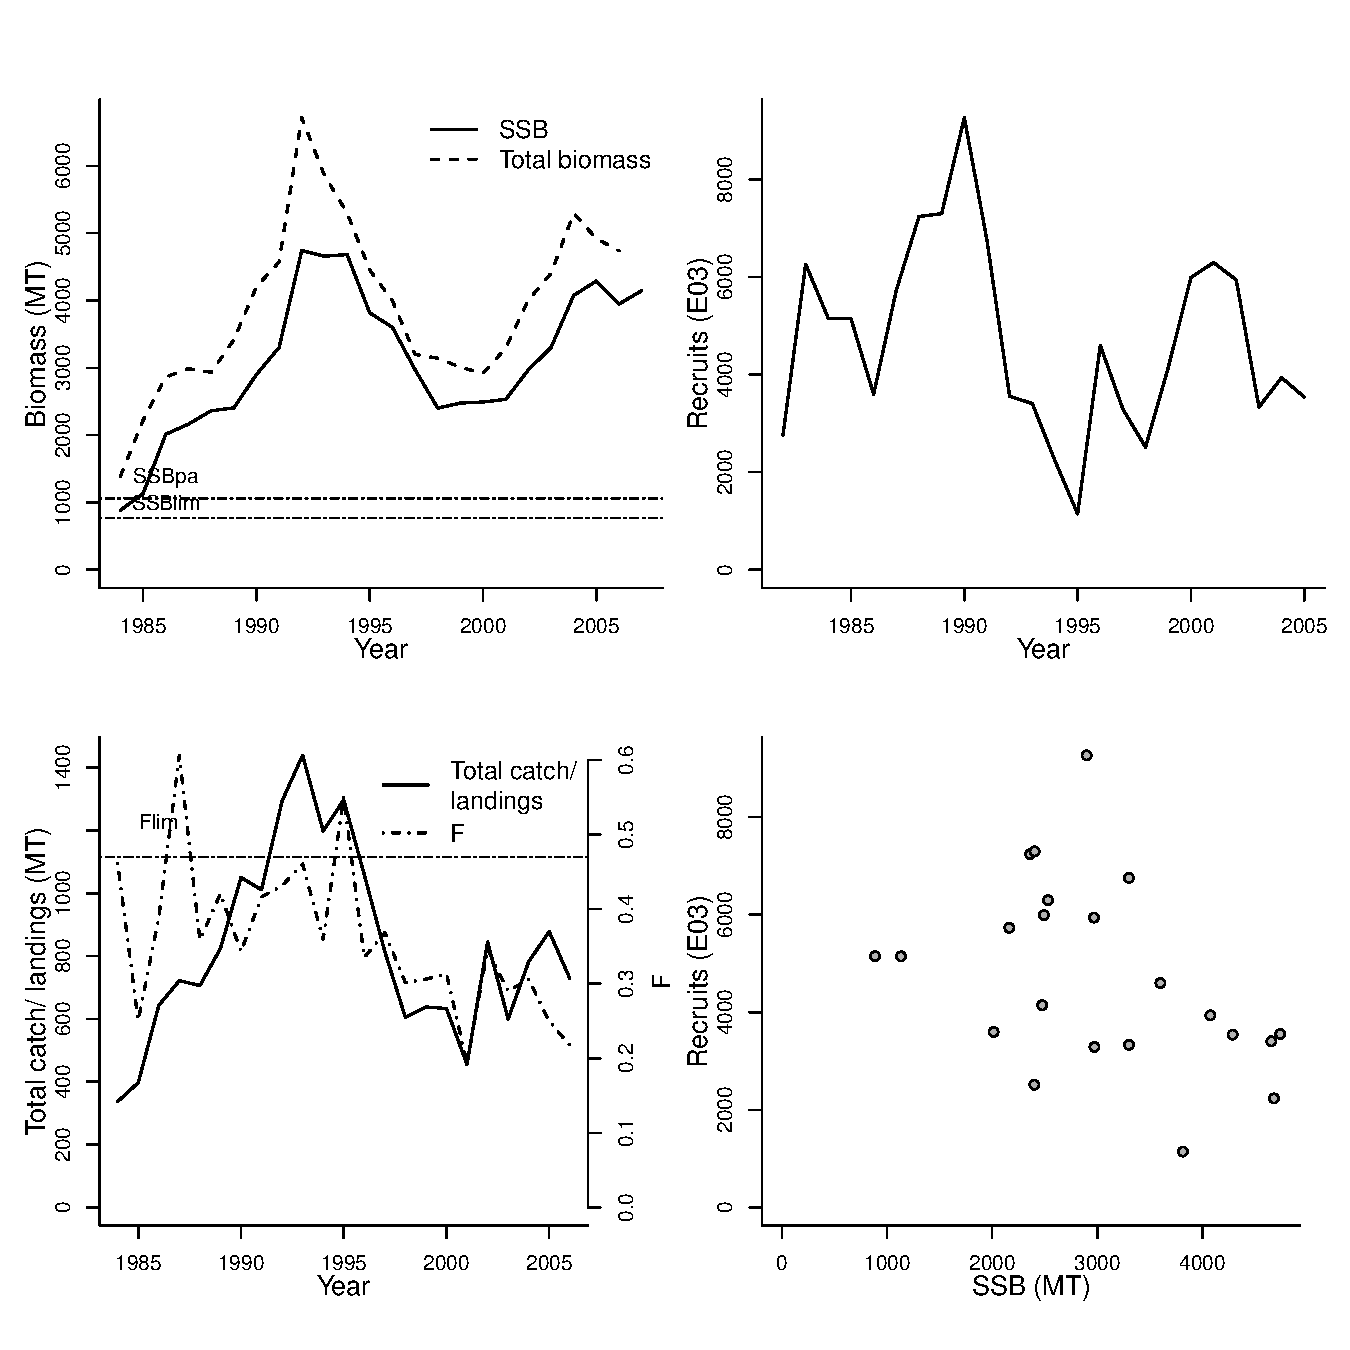
\includegraphics[scale=0.65]{../tex/figures/plot-WGBFAS-SOLEIIIa-1982-2007-JENNINGS.pdf}
\end{center}

\newpage
\subsubsection{Solea vulgaris - common European sole}\index{common European sole}\index{Solea vulgaris}\index{Soleidae!Solea vulgaris}
ID: WGSSDS-SOLEVIIe-1968-2006-JENNINGS

common European sole Western English Channel 

stock assessment conducted: Extended Survivor Analysis 
\begin{center}
\vspace{-0.2cm}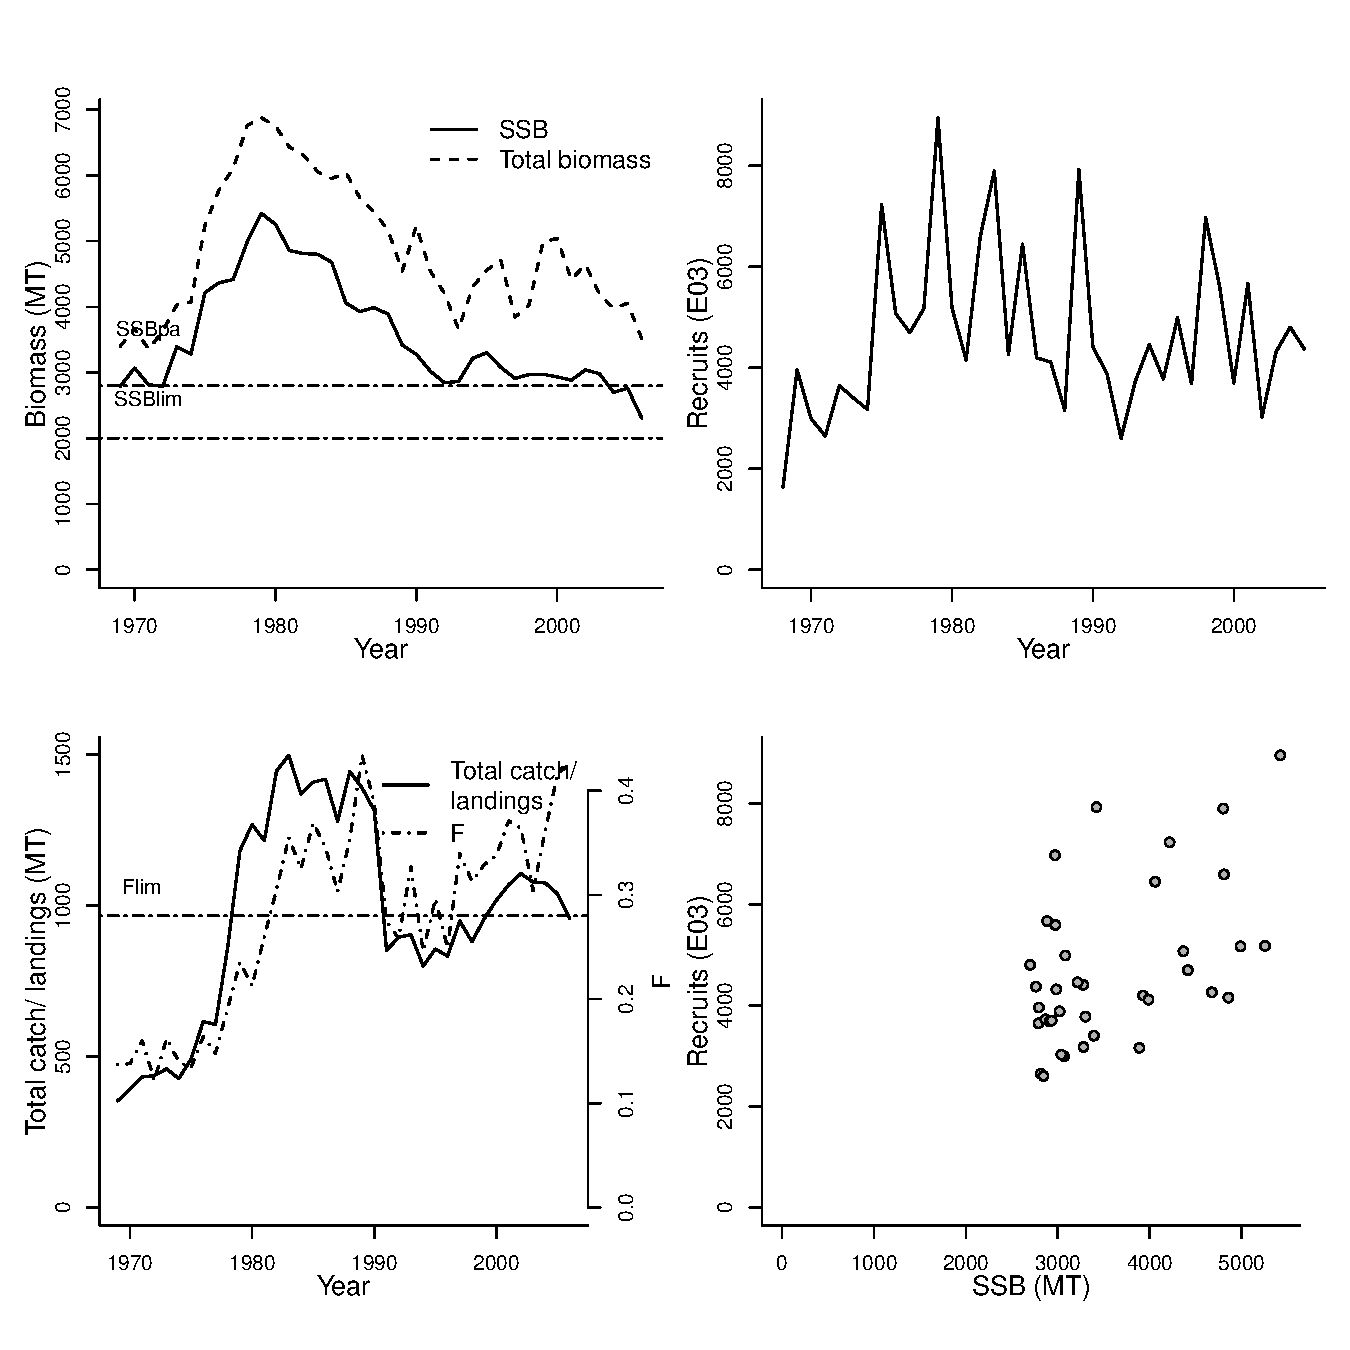
\includegraphics[scale=0.65]{../tex/figures/plot-WGSSDS-SOLEVIIe-1968-2006-JENNINGS.pdf}
\end{center}

\newpage
\section{Scorpaeniformes}\index{Scorpaeniformes}

\subsection{Scorpaenidae}\index{Scorpaenidae}\index{Scorpaeniformes!Scorpaenidae}

\subsubsection{Sebastes crameri - Darkblotched rockfish}\index{Darkblotched rockfish}\index{Sebastes crameri}\index{Scorpaenidae!Sebastes crameri}
ID: NWFSC-DKROCKPCOAST-1928-2007-BRANCH

Darkblotched rockfish Pacific Coast 

stock assessment conducted: Stock Synthesis v2.0 model 
\begin{center}
\vspace{-0.2cm}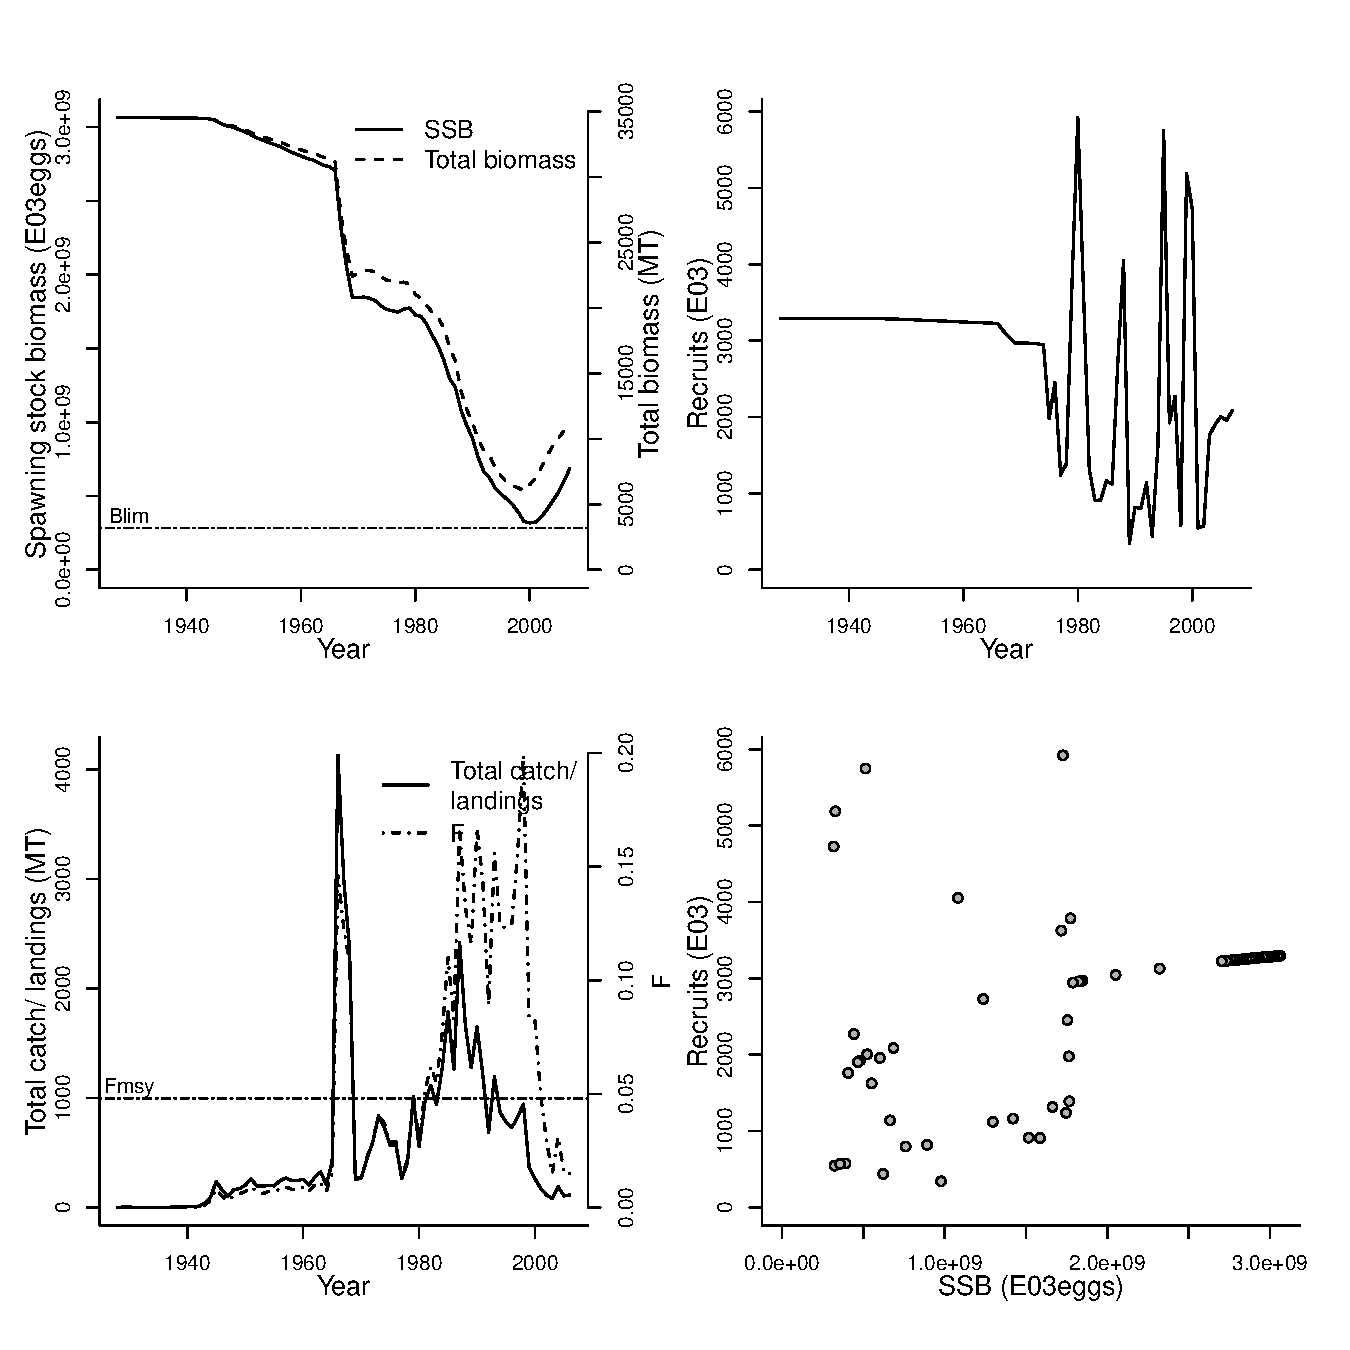
\includegraphics[scale=0.65]{../tex/figures/plot-NWFSC-DKROCKPCOAST-1928-2007-BRANCH.pdf}
\end{center}

\newpage
\subsubsection{Sebastes melanops - Black rockfish}\index{Black rockfish}\index{Sebastes melanops}\index{Scorpaenidae!Sebastes melanops}
ID: NWFSC-BLACKROCKNPCOAST-1914-2006-BRANCH

Black rockfish Northern Pacific Coast 

stock assessment conducted: Stock Synthesis v2.0 model 
\begin{center}
\vspace{-0.2cm}\includegraphics[scale=0.65]{../tex/figures/plot-NWFSC-BLACKROCKNPCOAST-1914-2006-BRANCH.pdf}
\end{center}

\newpage
\subsubsection{Sebastes melanops - Black rockfish}\index{Black rockfish}\index{Sebastes melanops}\index{Scorpaenidae!Sebastes melanops}
ID: NWFSC-BLACKROCKSPCOAST-1915-2007-BRANCH

Black rockfish Southern Pacific Coast 

stock assessment conducted: Stock Synthesis v2.0 model 
\begin{center}
\vspace{-0.2cm}\includegraphics[scale=0.65]{../tex/figures/plot-NWFSC-BLACKROCKSPCOAST-1915-2007-BRANCH.pdf}
\end{center}

\newpage
